\documentclass[twoside]{book}

% Packages required by doxygen
\usepackage{fixltx2e}
\usepackage{calc}
\usepackage{doxygen}
\usepackage[export]{adjustbox} % also loads graphicx
\usepackage{graphicx}
\usepackage[utf8]{inputenc}
\usepackage{makeidx}
\usepackage{multicol}
\usepackage{multirow}
\PassOptionsToPackage{warn}{textcomp}
\usepackage{textcomp}
\usepackage[nointegrals]{wasysym}
\usepackage[table]{xcolor}

% Font selection
\usepackage[T1]{fontenc}
\usepackage[scaled=.90]{helvet}
\usepackage{courier}
\usepackage{amssymb}
\usepackage{sectsty}
\renewcommand{\familydefault}{\sfdefault}
\allsectionsfont{%
  \fontseries{bc}\selectfont%
  \color{darkgray}%
}
\renewcommand{\DoxyLabelFont}{%
  \fontseries{bc}\selectfont%
  \color{darkgray}%
}
\newcommand{\+}{\discretionary{\mbox{\scriptsize$\hookleftarrow$}}{}{}}

% Page & text layout
\usepackage{geometry}
\geometry{%
  a4paper,%
  top=2.5cm,%
  bottom=2.5cm,%
  left=2.5cm,%
  right=2.5cm%
}
\tolerance=750
\hfuzz=15pt
\hbadness=750
\setlength{\emergencystretch}{15pt}
\setlength{\parindent}{0cm}
\setlength{\parskip}{3ex plus 2ex minus 2ex}
\makeatletter
\renewcommand{\paragraph}{%
  \@startsection{paragraph}{4}{0ex}{-1.0ex}{1.0ex}{%
    \normalfont\normalsize\bfseries\SS@parafont%
  }%
}
\renewcommand{\subparagraph}{%
  \@startsection{subparagraph}{5}{0ex}{-1.0ex}{1.0ex}{%
    \normalfont\normalsize\bfseries\SS@subparafont%
  }%
}
\makeatother

% Headers & footers
\usepackage{fancyhdr}
\pagestyle{fancyplain}
\fancyhead[LE]{\fancyplain{}{\bfseries\thepage}}
\fancyhead[CE]{\fancyplain{}{}}
\fancyhead[RE]{\fancyplain{}{\bfseries\leftmark}}
\fancyhead[LO]{\fancyplain{}{\bfseries\rightmark}}
\fancyhead[CO]{\fancyplain{}{}}
\fancyhead[RO]{\fancyplain{}{\bfseries\thepage}}
\fancyfoot[LE]{\fancyplain{}{}}
\fancyfoot[CE]{\fancyplain{}{}}
\fancyfoot[RE]{\fancyplain{}{\bfseries\scriptsize Generated by Doxygen }}
\fancyfoot[LO]{\fancyplain{}{\bfseries\scriptsize Generated by Doxygen }}
\fancyfoot[CO]{\fancyplain{}{}}
\fancyfoot[RO]{\fancyplain{}{}}
\renewcommand{\footrulewidth}{0.4pt}
\renewcommand{\chaptermark}[1]{%
  \markboth{#1}{}%
}
\renewcommand{\sectionmark}[1]{%
  \markright{\thesection\ #1}%
}

% Indices & bibliography
\usepackage{natbib}
\usepackage[titles]{tocloft}
\setcounter{tocdepth}{3}
\setcounter{secnumdepth}{5}
\makeindex

% Custom commands
\newcommand{\clearemptydoublepage}{%
  \newpage{\pagestyle{empty}\cleardoublepage}%
}

\usepackage{caption}
\captionsetup{labelsep=space,justification=centering,font={bf},singlelinecheck=off,skip=4pt,position=top}

%===== C O N T E N T S =====

\begin{document}

% Titlepage & ToC
\pagenumbering{alph}
\begin{titlepage}
\vspace*{7cm}
\begin{center}%
{\Large Software documentation -\/ W\+F\+YD A\+PI }\\
\vspace*{1cm}
{\large Generated by Doxygen 1.8.13}\\
\end{center}
\end{titlepage}
\clearemptydoublepage
\pagenumbering{roman}
\tableofcontents
\clearemptydoublepage
\pagenumbering{arabic}

%--- Begin generated contents ---
\chapter{qb\+A\+PI Libraries}
\label{index}This is the firmware of W\+F\+YD. \begin{DoxyVersion}{Version}
1.\+0
\end{DoxyVersion}
This is the firmware of the W\+F\+YD. It can control two motors and a servo motors and read their encoders. Also can read and convert analog measurements connected to the P\+SoC microcontroller. 
\chapter{Data Structure Index}
\section{Data Structures}
Here are the data structures with brief descriptions\+:\begin{DoxyCompactList}
\item\contentsline{section}{\textbf{ st\+\_\+data} }{\pageref{structst__data}}{}
\item\contentsline{section}{\textbf{ st\+\_\+meas} }{\pageref{structst__meas}}{}
\item\contentsline{section}{\textbf{ st\+\_\+mem} }{\pageref{structst__mem}}{}
\item\contentsline{section}{\textbf{ st\+\_\+ref} }{\pageref{structst__ref}}{}
\end{DoxyCompactList}

\chapter{File Index}
\section{File List}
Here is a list of all documented files with brief descriptions\+:\begin{DoxyCompactList}
\item\contentsline{section}{\textbf{ command\+\_\+processing.\+c} \\*Command processing functions }{\pageref{command__processing_8c}}{}
\item\contentsline{section}{\textbf{ command\+\_\+processing.\+h} \\*Command processing functions }{\pageref{command__processing_8h}}{}
\item\contentsline{section}{\textbf{ commands.\+h} \\*Definitions for commands, parameters and packages }{\pageref{commands_8h}}{}
\item\contentsline{section}{{\bfseries device.\+h} }{\pageref{device_8h}}{}
\item\contentsline{section}{\textbf{ globals.\+c} \\*Global variables }{\pageref{globals_8c}}{}
\item\contentsline{section}{\textbf{ globals.\+h} \\*Global definitions and macros are set in this file }{\pageref{globals_8h}}{}
\item\contentsline{section}{\textbf{ interruptions.\+c} \\*Interruption functions are in this file }{\pageref{interruptions_8c}}{}
\item\contentsline{section}{\textbf{ interruptions.\+h} \\*Interruptions header file }{\pageref{interruptions_8h}}{}
\item\contentsline{section}{\textbf{ main.\+c} \\*Firmware main file }{\pageref{main_8c}}{}
\item\contentsline{section}{\textbf{ utils.\+h} \\*Definition of utility functions }{\pageref{utils_8h}}{}
\end{DoxyCompactList}

\chapter{Data Structure Documentation}
\section{comm\+\_\+settings Struct Reference}
\label{structcomm__settings}\index{comm\+\_\+settings@{comm\+\_\+settings}}
\subsection*{Data Fields}
\begin{DoxyCompactItemize}
\item 
\mbox{\label{structcomm__settings_a577bde85e1667e1d14573add870f6fce}} 
H\+A\+N\+D\+LE {\bfseries file\+\_\+handle}
\end{DoxyCompactItemize}


The documentation for this struct was generated from the following file\+:\begin{DoxyCompactItemize}
\item 
\textbf{ qbmove\+\_\+communications.\+h}\end{DoxyCompactItemize}

\chapter{File Documentation}
\section{commands.\+h File Reference}
\label{commands_8h}\index{commands.\+h@{commands.\+h}}


Definitions for board commands, parameters and packages.  


This graph shows which files directly or indirectly include this file\+:
\nopagebreak
\begin{figure}[H]
\begin{center}
\leavevmode
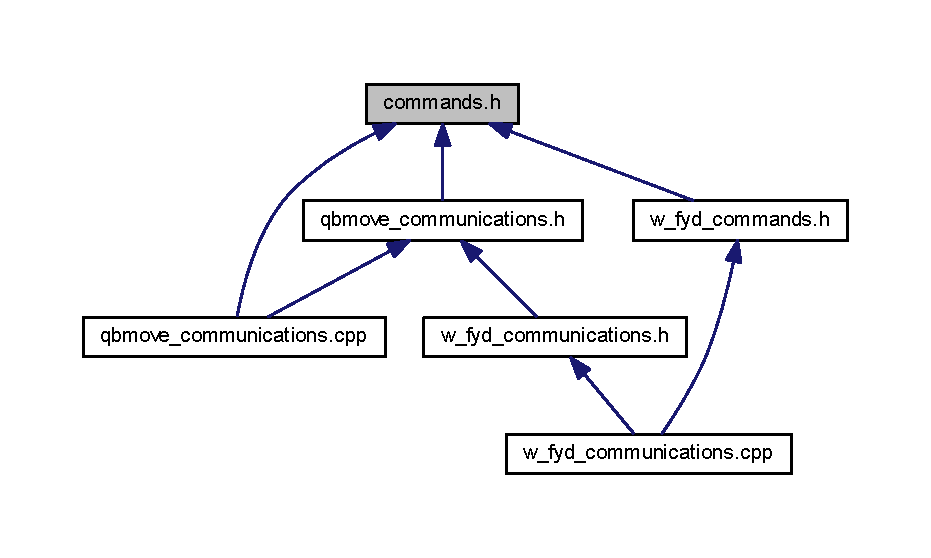
\includegraphics[width=350pt]{commands_8h__dep__incl}
\end{center}
\end{figure}
\subsection*{Macros}
\begin{DoxyCompactItemize}
\item 
\mbox{\label{commands_8h_ad97188edfdd667de971027b35330fa41}} 
\#define {\bfseries A\+P\+I\+\_\+\+V\+E\+R\+S\+I\+ON}~\char`\"{}v6.\+1.\+0\char`\"{}
\end{DoxyCompactItemize}
\begin{Indent}\textbf{ QB Move Information Strings}\par
\begin{DoxyCompactItemize}
\item 
\mbox{\label{commands_8h_a2ba44fc5b8a316bd307d0baa9ab629ef}} 
\#define \textbf{ I\+N\+F\+O\+\_\+\+A\+LL}~0
\begin{DoxyCompactList}\small\item\em All system information. \end{DoxyCompactList}\end{DoxyCompactItemize}
\end{Indent}
\subsection*{Enumerations}
\begin{Indent}\textbf{ qb\+Move and qb\+Hand Commands}\par
\begin{DoxyCompactItemize}
\item 
enum \textbf{ qbmove\+\_\+command} \{ \newline
\textbf{ C\+M\+D\+\_\+\+P\+I\+NG} = 0, 
\textbf{ C\+M\+D\+\_\+\+S\+E\+T\+\_\+\+Z\+E\+R\+OS} = 1, 
\textbf{ C\+M\+D\+\_\+\+S\+T\+O\+R\+E\+\_\+\+P\+A\+R\+A\+MS} = 3, 
\textbf{ C\+M\+D\+\_\+\+S\+T\+O\+R\+E\+\_\+\+D\+E\+F\+A\+U\+L\+T\+\_\+\+P\+A\+R\+A\+MS} = 4, 
\newline
\textbf{ C\+M\+D\+\_\+\+R\+E\+S\+T\+O\+R\+E\+\_\+\+P\+A\+R\+A\+MS} = 5, 
\textbf{ C\+M\+D\+\_\+\+G\+E\+T\+\_\+\+I\+N\+FO} = 6, 
\textbf{ C\+M\+D\+\_\+\+S\+E\+T\+\_\+\+V\+A\+L\+UE} = 7, 
\textbf{ C\+M\+D\+\_\+\+G\+E\+T\+\_\+\+V\+A\+L\+UE} = 8, 
\newline
\textbf{ C\+M\+D\+\_\+\+B\+O\+O\+T\+L\+O\+A\+D\+ER} = 9, 
\textbf{ C\+M\+D\+\_\+\+I\+N\+I\+T\+\_\+\+M\+EM} = 10, 
\textbf{ C\+M\+D\+\_\+\+C\+A\+L\+I\+B\+R\+A\+TE} = 11, 
\textbf{ C\+M\+D\+\_\+\+G\+E\+T\+\_\+\+P\+A\+R\+A\+M\+\_\+\+L\+I\+ST} = 12, 
\newline
\textbf{ C\+M\+D\+\_\+\+H\+A\+N\+D\+\_\+\+C\+A\+L\+I\+B\+R\+A\+TE} = 13, 
\textbf{ C\+M\+D\+\_\+\+A\+C\+T\+I\+V\+A\+TE} = 128, 
\textbf{ C\+M\+D\+\_\+\+G\+E\+T\+\_\+\+A\+C\+T\+I\+V\+A\+TE} = 129, 
\textbf{ C\+M\+D\+\_\+\+S\+E\+T\+\_\+\+I\+N\+P\+U\+TS} = 130, 
\newline
\textbf{ C\+M\+D\+\_\+\+G\+E\+T\+\_\+\+I\+N\+P\+U\+TS} = 131, 
\textbf{ C\+M\+D\+\_\+\+G\+E\+T\+\_\+\+M\+E\+A\+S\+U\+R\+E\+M\+E\+N\+TS} = 132, 
\textbf{ C\+M\+D\+\_\+\+G\+E\+T\+\_\+\+C\+U\+R\+R\+E\+N\+TS} = 133, 
\textbf{ C\+M\+D\+\_\+\+G\+E\+T\+\_\+\+C\+U\+R\+R\+\_\+\+A\+N\+D\+\_\+\+M\+E\+AS} = 134, 
\newline
\textbf{ C\+M\+D\+\_\+\+S\+E\+T\+\_\+\+P\+O\+S\+\_\+\+S\+T\+I\+FF} = 135, 
\textbf{ C\+M\+D\+\_\+\+G\+E\+T\+\_\+\+E\+MG} = 136, 
\textbf{ C\+M\+D\+\_\+\+G\+E\+T\+\_\+\+V\+E\+L\+O\+C\+I\+T\+I\+ES} = 137, 
\textbf{ C\+M\+D\+\_\+\+G\+E\+T\+\_\+\+C\+O\+U\+N\+T\+E\+RS} = 138, 
\newline
\textbf{ C\+M\+D\+\_\+\+G\+E\+T\+\_\+\+A\+C\+C\+EL} = 139, 
\textbf{ C\+M\+D\+\_\+\+G\+E\+T\+\_\+\+C\+U\+R\+R\+\_\+\+D\+I\+FF} = 140, 
\textbf{ C\+M\+D\+\_\+\+S\+E\+T\+\_\+\+C\+U\+R\+R\+\_\+\+D\+I\+FF} = 141, 
\textbf{ C\+M\+D\+\_\+\+S\+E\+T\+\_\+\+C\+U\+F\+F\+\_\+\+I\+N\+P\+U\+TS} = 142, 
\newline
\textbf{ C\+M\+D\+\_\+\+S\+E\+T\+\_\+\+W\+A\+T\+C\+H\+D\+OG} = 143, 
\textbf{ C\+M\+D\+\_\+\+S\+E\+T\+\_\+\+B\+A\+U\+D\+R\+A\+TE} = 144, 
\textbf{ C\+M\+D\+\_\+\+E\+X\+T\+\_\+\+D\+R\+I\+VE} = 145, 
\textbf{ C\+M\+D\+\_\+\+G\+E\+T\+\_\+\+J\+O\+Y\+S\+T\+I\+CK} = 146
 \}
\end{DoxyCompactItemize}
\end{Indent}
\subsection*{qb\+Move and qb\+Hand Parameters}
\begin{DoxyCompactItemize}
\item 
\mbox{\label{commands_8h_ae3302107827a773be3200e459e7b24da}} 
\#define {\bfseries P\+A\+R\+A\+M\+\_\+\+B\+Y\+T\+E\+\_\+\+S\+L\+OT}~50
\item 
\mbox{\label{commands_8h_a3bab5133f6aa363d84307b39e17b0d74}} 
\#define {\bfseries P\+A\+R\+A\+M\+\_\+\+M\+E\+N\+U\+\_\+\+S\+L\+OT}~150
\item 
enum \textbf{ qbmove\+\_\+parameter} \{ \newline
\textbf{ P\+A\+R\+A\+M\+\_\+\+ID} = 0, 
\textbf{ P\+A\+R\+A\+M\+\_\+\+P\+I\+D\+\_\+\+C\+O\+N\+T\+R\+OL} = 1, 
\textbf{ P\+A\+R\+A\+M\+\_\+\+S\+T\+A\+R\+T\+U\+P\+\_\+\+A\+C\+T\+I\+V\+A\+T\+I\+ON} = 2, 
\textbf{ P\+A\+R\+A\+M\+\_\+\+I\+N\+P\+U\+T\+\_\+\+M\+O\+DE} = 3, 
\newline
\textbf{ P\+A\+R\+A\+M\+\_\+\+C\+O\+N\+T\+R\+O\+L\+\_\+\+M\+O\+DE} = 4, 
\textbf{ P\+A\+R\+A\+M\+\_\+\+M\+E\+A\+S\+U\+R\+E\+M\+E\+N\+T\+\_\+\+O\+F\+F\+S\+ET} = 5, 
\textbf{ P\+A\+R\+A\+M\+\_\+\+M\+E\+A\+S\+U\+R\+E\+M\+E\+N\+T\+\_\+\+M\+U\+L\+T\+I\+P\+L\+I\+ER} = 6, 
\textbf{ P\+A\+R\+A\+M\+\_\+\+P\+O\+S\+\_\+\+L\+I\+M\+I\+T\+\_\+\+F\+L\+AG} = 7, 
\newline
\textbf{ P\+A\+R\+A\+M\+\_\+\+P\+O\+S\+\_\+\+L\+I\+M\+IT} = 8, 
\textbf{ P\+A\+R\+A\+M\+\_\+\+M\+A\+X\+\_\+\+S\+T\+E\+P\+\_\+\+P\+OS} = 9, 
\textbf{ P\+A\+R\+A\+M\+\_\+\+M\+A\+X\+\_\+\+S\+T\+E\+P\+\_\+\+N\+EG} = 10, 
\textbf{ P\+A\+R\+A\+M\+\_\+\+P\+O\+S\+\_\+\+R\+E\+S\+O\+L\+U\+T\+I\+ON} = 11, 
\newline
\textbf{ P\+A\+R\+A\+M\+\_\+\+C\+U\+R\+R\+E\+N\+T\+\_\+\+L\+I\+M\+IT} = 12, 
\textbf{ P\+A\+R\+A\+M\+\_\+\+E\+M\+G\+\_\+\+C\+A\+L\+I\+B\+\_\+\+F\+L\+AG} = 13, 
\textbf{ P\+A\+R\+A\+M\+\_\+\+E\+M\+G\+\_\+\+T\+H\+R\+E\+S\+H\+O\+LD} = 14, 
\textbf{ P\+A\+R\+A\+M\+\_\+\+E\+M\+G\+\_\+\+M\+A\+X\+\_\+\+V\+A\+L\+UE} = 15, 
\newline
\textbf{ P\+A\+R\+A\+M\+\_\+\+E\+M\+G\+\_\+\+S\+P\+E\+ED} = 16, 
\textbf{ P\+A\+R\+A\+M\+\_\+\+P\+I\+D\+\_\+\+C\+U\+R\+R\+\_\+\+C\+O\+N\+T\+R\+OL} = 18, 
\textbf{ P\+A\+R\+A\+M\+\_\+\+D\+O\+U\+B\+L\+E\+\_\+\+E\+N\+C\+\_\+\+O\+N\+\_\+\+O\+FF} = 19, 
\textbf{ P\+A\+R\+A\+M\+\_\+\+M\+O\+T\+\_\+\+H\+A\+N\+D\+L\+E\+\_\+\+R\+A\+T\+IO} = 20, 
\newline
\textbf{ P\+A\+R\+A\+M\+\_\+\+M\+O\+T\+O\+R\+\_\+\+S\+U\+P\+P\+LY} = 21, 
\textbf{ P\+A\+R\+A\+M\+\_\+\+C\+U\+R\+R\+E\+N\+T\+\_\+\+L\+O\+O\+K\+UP} = 23, 
\textbf{ P\+A\+R\+A\+M\+\_\+\+D\+L\+\_\+\+P\+O\+S\+\_\+\+P\+ID} = 24, 
\textbf{ P\+A\+R\+A\+M\+\_\+\+D\+L\+\_\+\+C\+U\+R\+R\+\_\+\+P\+ID} = 25
 \}
\item 
\mbox{\label{commands_8h_ad18f2ef316ee226b52882af5758c39e8}} 
enum {\bfseries qbmove\+\_\+resolution} \{ \newline
{\bfseries R\+E\+S\+O\+L\+U\+T\+I\+O\+N\+\_\+360} = 0, 
{\bfseries R\+E\+S\+O\+L\+U\+T\+I\+O\+N\+\_\+720} = 1, 
{\bfseries R\+E\+S\+O\+L\+U\+T\+I\+O\+N\+\_\+1440} = 2, 
{\bfseries R\+E\+S\+O\+L\+U\+T\+I\+O\+N\+\_\+2880} = 3, 
\newline
{\bfseries R\+E\+S\+O\+L\+U\+T\+I\+O\+N\+\_\+5760} = 4, 
{\bfseries R\+E\+S\+O\+L\+U\+T\+I\+O\+N\+\_\+11520} = 5, 
{\bfseries R\+E\+S\+O\+L\+U\+T\+I\+O\+N\+\_\+23040} = 6, 
{\bfseries R\+E\+S\+O\+L\+U\+T\+I\+O\+N\+\_\+46080} = 7, 
\newline
{\bfseries R\+E\+S\+O\+L\+U\+T\+I\+O\+N\+\_\+92160} = 8
 \}
\item 
enum \textbf{ qbmove\+\_\+input\+\_\+mode} \{ \newline
\textbf{ I\+N\+P\+U\+T\+\_\+\+M\+O\+D\+E\+\_\+\+E\+X\+T\+E\+R\+N\+AL} = 0, 
\textbf{ I\+N\+P\+U\+T\+\_\+\+M\+O\+D\+E\+\_\+\+E\+N\+C\+O\+D\+E\+R3} = 1, 
\textbf{ I\+N\+P\+U\+T\+\_\+\+M\+O\+D\+E\+\_\+\+E\+M\+G\+\_\+\+P\+R\+O\+P\+O\+R\+T\+I\+O\+N\+AL} = 2, 
\textbf{ I\+N\+P\+U\+T\+\_\+\+M\+O\+D\+E\+\_\+\+E\+M\+G\+\_\+\+I\+N\+T\+E\+G\+R\+AL} = 3, 
\newline
\textbf{ I\+N\+P\+U\+T\+\_\+\+M\+O\+D\+E\+\_\+\+E\+M\+G\+\_\+\+F\+C\+FS} = 4, 
\textbf{ I\+N\+P\+U\+T\+\_\+\+M\+O\+D\+E\+\_\+\+E\+M\+G\+\_\+\+F\+C\+F\+S\+\_\+\+A\+DV} = 5
 \}
\item 
enum \textbf{ qbmove\+\_\+control\+\_\+mode} \{ \newline
\textbf{ C\+O\+N\+T\+R\+O\+L\+\_\+\+A\+N\+G\+LE} = 0, 
\textbf{ C\+O\+N\+T\+R\+O\+L\+\_\+\+P\+WM} = 1, 
\textbf{ C\+O\+N\+T\+R\+O\+L\+\_\+\+C\+U\+R\+R\+E\+NT} = 2, 
\textbf{ C\+U\+R\+R\+\_\+\+A\+N\+D\+\_\+\+P\+O\+S\+\_\+\+C\+O\+N\+T\+R\+OL} = 3, 
\newline
\textbf{ D\+E\+F\+L\+E\+C\+T\+I\+O\+N\+\_\+\+C\+O\+N\+T\+R\+OL} = 4, 
\textbf{ D\+E\+F\+L\+\_\+\+C\+U\+R\+R\+E\+N\+T\+\_\+\+C\+O\+N\+T\+R\+OL} = 5
 \}
\item 
\mbox{\label{commands_8h_a17c218160a8b2c5f25db27616793d564}} 
enum {\bfseries motor\+\_\+supply\+\_\+tipe} \{ {\bfseries M\+A\+X\+O\+N\+\_\+24V} = 0, 
{\bfseries M\+A\+X\+O\+N\+\_\+12V} = 1
 \}
\item 
\mbox{\label{commands_8h_a0eae1c82d20671c5d0b9b82b10070f1b}} 
enum {\bfseries acknowledgment\+\_\+values} \{ {\bfseries A\+C\+K\+\_\+\+E\+R\+R\+OR} = 0, 
{\bfseries A\+C\+K\+\_\+\+OK} = 1
 \}
\item 
\mbox{\label{commands_8h_aee7544e5fa6e2843ecdc3609602e56aa}} 
enum {\bfseries data\+\_\+types} \{ \newline
{\bfseries T\+Y\+P\+E\+\_\+\+F\+L\+AG} = 0, 
{\bfseries T\+Y\+P\+E\+\_\+\+I\+N\+T8} = 1, 
{\bfseries T\+Y\+P\+E\+\_\+\+U\+I\+N\+T8} = 2, 
{\bfseries T\+Y\+P\+E\+\_\+\+I\+N\+T16} = 3, 
\newline
{\bfseries T\+Y\+P\+E\+\_\+\+U\+I\+N\+T16} = 4, 
{\bfseries T\+Y\+P\+E\+\_\+\+I\+N\+T32} = 5, 
{\bfseries T\+Y\+P\+E\+\_\+\+U\+I\+N\+T32} = 6, 
{\bfseries T\+Y\+P\+E\+\_\+\+F\+L\+O\+AT} = 7, 
\newline
{\bfseries T\+Y\+P\+E\+\_\+\+D\+O\+U\+B\+LE} = 8
 \}
\end{DoxyCompactItemize}


\subsection{Detailed Description}
Definitions for board commands, parameters and packages. 

\begin{DoxyAuthor}{Author}
{\itshape Centro \char`\"{}\+E.\+Piaggio\char`\"{}} 
\end{DoxyAuthor}
\begin{DoxyCopyright}{Copyright}
(C) 2012-\/2016 qbrobotics. All rights reserved. 

(C) 2017 Centro \char`\"{}\+E.\+Piaggio\char`\"{}. All rights reserved.
\end{DoxyCopyright}
This file is included in the board firmware, in its libraries and applications. It contains all definitions that are necessary for the contruction of communication packages.

It includes definitions for all of the device commands, parameters and also the size of answer packages. 

\subsection{Enumeration Type Documentation}
\mbox{\label{commands_8h_abf0494aabdc65d654a54044eddc9210b}} 
\index{commands.\+h@{commands.\+h}!qbmove\+\_\+command@{qbmove\+\_\+command}}
\index{qbmove\+\_\+command@{qbmove\+\_\+command}!commands.\+h@{commands.\+h}}
\subsubsection{qbmove\+\_\+command}
{\footnotesize\ttfamily enum \textbf{ qbmove\+\_\+command}}

\begin{DoxyEnumFields}{Enumerator}
\raisebox{\heightof{T}}[0pt][0pt]{\index{C\+M\+D\+\_\+\+P\+I\+NG@{C\+M\+D\+\_\+\+P\+I\+NG}!commands.\+h@{commands.\+h}}\index{commands.\+h@{commands.\+h}!C\+M\+D\+\_\+\+P\+I\+NG@{C\+M\+D\+\_\+\+P\+I\+NG}}}\mbox{\label{commands_8h_abf0494aabdc65d654a54044eddc9210ba1c0aa24c3612e77ea1a5ca1b82388da0}} 
C\+M\+D\+\_\+\+P\+I\+NG&Asks for a ping message. \\
\hline

\raisebox{\heightof{T}}[0pt][0pt]{\index{C\+M\+D\+\_\+\+S\+E\+T\+\_\+\+Z\+E\+R\+OS@{C\+M\+D\+\_\+\+S\+E\+T\+\_\+\+Z\+E\+R\+OS}!commands.\+h@{commands.\+h}}\index{commands.\+h@{commands.\+h}!C\+M\+D\+\_\+\+S\+E\+T\+\_\+\+Z\+E\+R\+OS@{C\+M\+D\+\_\+\+S\+E\+T\+\_\+\+Z\+E\+R\+OS}}}\mbox{\label{commands_8h_abf0494aabdc65d654a54044eddc9210ba2d92e89157e03fe63bfebf8125c3a0d7}} 
C\+M\+D\+\_\+\+S\+E\+T\+\_\+\+Z\+E\+R\+OS&Command for setting the encoders zero position. \\
\hline

\raisebox{\heightof{T}}[0pt][0pt]{\index{C\+M\+D\+\_\+\+S\+T\+O\+R\+E\+\_\+\+P\+A\+R\+A\+MS@{C\+M\+D\+\_\+\+S\+T\+O\+R\+E\+\_\+\+P\+A\+R\+A\+MS}!commands.\+h@{commands.\+h}}\index{commands.\+h@{commands.\+h}!C\+M\+D\+\_\+\+S\+T\+O\+R\+E\+\_\+\+P\+A\+R\+A\+MS@{C\+M\+D\+\_\+\+S\+T\+O\+R\+E\+\_\+\+P\+A\+R\+A\+MS}}}\mbox{\label{commands_8h_abf0494aabdc65d654a54044eddc9210bac7d1170961179d8dc5ec1b4aeb4f3116}} 
C\+M\+D\+\_\+\+S\+T\+O\+R\+E\+\_\+\+P\+A\+R\+A\+MS&Stores all parameters in memory and loads them \\
\hline

\raisebox{\heightof{T}}[0pt][0pt]{\index{C\+M\+D\+\_\+\+S\+T\+O\+R\+E\+\_\+\+D\+E\+F\+A\+U\+L\+T\+\_\+\+P\+A\+R\+A\+MS@{C\+M\+D\+\_\+\+S\+T\+O\+R\+E\+\_\+\+D\+E\+F\+A\+U\+L\+T\+\_\+\+P\+A\+R\+A\+MS}!commands.\+h@{commands.\+h}}\index{commands.\+h@{commands.\+h}!C\+M\+D\+\_\+\+S\+T\+O\+R\+E\+\_\+\+D\+E\+F\+A\+U\+L\+T\+\_\+\+P\+A\+R\+A\+MS@{C\+M\+D\+\_\+\+S\+T\+O\+R\+E\+\_\+\+D\+E\+F\+A\+U\+L\+T\+\_\+\+P\+A\+R\+A\+MS}}}\mbox{\label{commands_8h_abf0494aabdc65d654a54044eddc9210ba17d9c730cd01059737de14b9f062e44c}} 
C\+M\+D\+\_\+\+S\+T\+O\+R\+E\+\_\+\+D\+E\+F\+A\+U\+L\+T\+\_\+\+P\+A\+R\+A\+MS&Store current parameters as factory parameters. \\
\hline

\raisebox{\heightof{T}}[0pt][0pt]{\index{C\+M\+D\+\_\+\+R\+E\+S\+T\+O\+R\+E\+\_\+\+P\+A\+R\+A\+MS@{C\+M\+D\+\_\+\+R\+E\+S\+T\+O\+R\+E\+\_\+\+P\+A\+R\+A\+MS}!commands.\+h@{commands.\+h}}\index{commands.\+h@{commands.\+h}!C\+M\+D\+\_\+\+R\+E\+S\+T\+O\+R\+E\+\_\+\+P\+A\+R\+A\+MS@{C\+M\+D\+\_\+\+R\+E\+S\+T\+O\+R\+E\+\_\+\+P\+A\+R\+A\+MS}}}\mbox{\label{commands_8h_abf0494aabdc65d654a54044eddc9210ba7f13c143f54c74572776ffae219d33d7}} 
C\+M\+D\+\_\+\+R\+E\+S\+T\+O\+R\+E\+\_\+\+P\+A\+R\+A\+MS&Restore default factory parameters. \\
\hline

\raisebox{\heightof{T}}[0pt][0pt]{\index{C\+M\+D\+\_\+\+G\+E\+T\+\_\+\+I\+N\+FO@{C\+M\+D\+\_\+\+G\+E\+T\+\_\+\+I\+N\+FO}!commands.\+h@{commands.\+h}}\index{commands.\+h@{commands.\+h}!C\+M\+D\+\_\+\+G\+E\+T\+\_\+\+I\+N\+FO@{C\+M\+D\+\_\+\+G\+E\+T\+\_\+\+I\+N\+FO}}}\mbox{\label{commands_8h_abf0494aabdc65d654a54044eddc9210ba4681b714888632a2d8ad0a2140e4ba7f}} 
C\+M\+D\+\_\+\+G\+E\+T\+\_\+\+I\+N\+FO&Asks for a string of information about. \\
\hline

\raisebox{\heightof{T}}[0pt][0pt]{\index{C\+M\+D\+\_\+\+S\+E\+T\+\_\+\+V\+A\+L\+UE@{C\+M\+D\+\_\+\+S\+E\+T\+\_\+\+V\+A\+L\+UE}!commands.\+h@{commands.\+h}}\index{commands.\+h@{commands.\+h}!C\+M\+D\+\_\+\+S\+E\+T\+\_\+\+V\+A\+L\+UE@{C\+M\+D\+\_\+\+S\+E\+T\+\_\+\+V\+A\+L\+UE}}}\mbox{\label{commands_8h_abf0494aabdc65d654a54044eddc9210bac3ca8989b510cb78baff4425a0d47a67}} 
C\+M\+D\+\_\+\+S\+E\+T\+\_\+\+V\+A\+L\+UE&Not Used. \\
\hline

\raisebox{\heightof{T}}[0pt][0pt]{\index{C\+M\+D\+\_\+\+G\+E\+T\+\_\+\+V\+A\+L\+UE@{C\+M\+D\+\_\+\+G\+E\+T\+\_\+\+V\+A\+L\+UE}!commands.\+h@{commands.\+h}}\index{commands.\+h@{commands.\+h}!C\+M\+D\+\_\+\+G\+E\+T\+\_\+\+V\+A\+L\+UE@{C\+M\+D\+\_\+\+G\+E\+T\+\_\+\+V\+A\+L\+UE}}}\mbox{\label{commands_8h_abf0494aabdc65d654a54044eddc9210bac9a592ed746a114c7bfc0bd9d094263c}} 
C\+M\+D\+\_\+\+G\+E\+T\+\_\+\+V\+A\+L\+UE&Not Used. \\
\hline

\raisebox{\heightof{T}}[0pt][0pt]{\index{C\+M\+D\+\_\+\+B\+O\+O\+T\+L\+O\+A\+D\+ER@{C\+M\+D\+\_\+\+B\+O\+O\+T\+L\+O\+A\+D\+ER}!commands.\+h@{commands.\+h}}\index{commands.\+h@{commands.\+h}!C\+M\+D\+\_\+\+B\+O\+O\+T\+L\+O\+A\+D\+ER@{C\+M\+D\+\_\+\+B\+O\+O\+T\+L\+O\+A\+D\+ER}}}\mbox{\label{commands_8h_abf0494aabdc65d654a54044eddc9210bac72c6075e3464ea5abbe0c0d6e11559e}} 
C\+M\+D\+\_\+\+B\+O\+O\+T\+L\+O\+A\+D\+ER&Sets the bootloader modality to update the firmware \\
\hline

\raisebox{\heightof{T}}[0pt][0pt]{\index{C\+M\+D\+\_\+\+I\+N\+I\+T\+\_\+\+M\+EM@{C\+M\+D\+\_\+\+I\+N\+I\+T\+\_\+\+M\+EM}!commands.\+h@{commands.\+h}}\index{commands.\+h@{commands.\+h}!C\+M\+D\+\_\+\+I\+N\+I\+T\+\_\+\+M\+EM@{C\+M\+D\+\_\+\+I\+N\+I\+T\+\_\+\+M\+EM}}}\mbox{\label{commands_8h_abf0494aabdc65d654a54044eddc9210ba7bd24a7ad88af9a4e7c398a9ecb08ed4}} 
C\+M\+D\+\_\+\+I\+N\+I\+T\+\_\+\+M\+EM&Initialize the memory with the defalut values. \\
\hline

\raisebox{\heightof{T}}[0pt][0pt]{\index{C\+M\+D\+\_\+\+C\+A\+L\+I\+B\+R\+A\+TE@{C\+M\+D\+\_\+\+C\+A\+L\+I\+B\+R\+A\+TE}!commands.\+h@{commands.\+h}}\index{commands.\+h@{commands.\+h}!C\+M\+D\+\_\+\+C\+A\+L\+I\+B\+R\+A\+TE@{C\+M\+D\+\_\+\+C\+A\+L\+I\+B\+R\+A\+TE}}}\mbox{\label{commands_8h_abf0494aabdc65d654a54044eddc9210ba238830aded332d3bd5cbbb4ea2cb6ce7}} 
C\+M\+D\+\_\+\+C\+A\+L\+I\+B\+R\+A\+TE&Starts the stiffness calibration of the qb\+Move. \\
\hline

\raisebox{\heightof{T}}[0pt][0pt]{\index{C\+M\+D\+\_\+\+G\+E\+T\+\_\+\+P\+A\+R\+A\+M\+\_\+\+L\+I\+ST@{C\+M\+D\+\_\+\+G\+E\+T\+\_\+\+P\+A\+R\+A\+M\+\_\+\+L\+I\+ST}!commands.\+h@{commands.\+h}}\index{commands.\+h@{commands.\+h}!C\+M\+D\+\_\+\+G\+E\+T\+\_\+\+P\+A\+R\+A\+M\+\_\+\+L\+I\+ST@{C\+M\+D\+\_\+\+G\+E\+T\+\_\+\+P\+A\+R\+A\+M\+\_\+\+L\+I\+ST}}}\mbox{\label{commands_8h_abf0494aabdc65d654a54044eddc9210ba3e92a6e4c288be3abb6f3cfadf261e78}} 
C\+M\+D\+\_\+\+G\+E\+T\+\_\+\+P\+A\+R\+A\+M\+\_\+\+L\+I\+ST&Command to get the parameters list or to set a defined value chosen by the use \\
\hline

\raisebox{\heightof{T}}[0pt][0pt]{\index{C\+M\+D\+\_\+\+H\+A\+N\+D\+\_\+\+C\+A\+L\+I\+B\+R\+A\+TE@{C\+M\+D\+\_\+\+H\+A\+N\+D\+\_\+\+C\+A\+L\+I\+B\+R\+A\+TE}!commands.\+h@{commands.\+h}}\index{commands.\+h@{commands.\+h}!C\+M\+D\+\_\+\+H\+A\+N\+D\+\_\+\+C\+A\+L\+I\+B\+R\+A\+TE@{C\+M\+D\+\_\+\+H\+A\+N\+D\+\_\+\+C\+A\+L\+I\+B\+R\+A\+TE}}}\mbox{\label{commands_8h_abf0494aabdc65d654a54044eddc9210ba76be5a50e0ac4a9f944d0d6382f06e92}} 
C\+M\+D\+\_\+\+H\+A\+N\+D\+\_\+\+C\+A\+L\+I\+B\+R\+A\+TE&Starts a series of opening and closures of the hand. \\
\hline

\raisebox{\heightof{T}}[0pt][0pt]{\index{C\+M\+D\+\_\+\+A\+C\+T\+I\+V\+A\+TE@{C\+M\+D\+\_\+\+A\+C\+T\+I\+V\+A\+TE}!commands.\+h@{commands.\+h}}\index{commands.\+h@{commands.\+h}!C\+M\+D\+\_\+\+A\+C\+T\+I\+V\+A\+TE@{C\+M\+D\+\_\+\+A\+C\+T\+I\+V\+A\+TE}}}\mbox{\label{commands_8h_abf0494aabdc65d654a54044eddc9210ba341cc0e29a584b4c75a7502529920a7f}} 
C\+M\+D\+\_\+\+A\+C\+T\+I\+V\+A\+TE&Command for activating/deactivating the device \\
\hline

\raisebox{\heightof{T}}[0pt][0pt]{\index{C\+M\+D\+\_\+\+G\+E\+T\+\_\+\+A\+C\+T\+I\+V\+A\+TE@{C\+M\+D\+\_\+\+G\+E\+T\+\_\+\+A\+C\+T\+I\+V\+A\+TE}!commands.\+h@{commands.\+h}}\index{commands.\+h@{commands.\+h}!C\+M\+D\+\_\+\+G\+E\+T\+\_\+\+A\+C\+T\+I\+V\+A\+TE@{C\+M\+D\+\_\+\+G\+E\+T\+\_\+\+A\+C\+T\+I\+V\+A\+TE}}}\mbox{\label{commands_8h_abf0494aabdc65d654a54044eddc9210bac56c7ee3592b79204a8f209460ca6531}} 
C\+M\+D\+\_\+\+G\+E\+T\+\_\+\+A\+C\+T\+I\+V\+A\+TE&Command for getting device activation state \\
\hline

\raisebox{\heightof{T}}[0pt][0pt]{\index{C\+M\+D\+\_\+\+S\+E\+T\+\_\+\+I\+N\+P\+U\+TS@{C\+M\+D\+\_\+\+S\+E\+T\+\_\+\+I\+N\+P\+U\+TS}!commands.\+h@{commands.\+h}}\index{commands.\+h@{commands.\+h}!C\+M\+D\+\_\+\+S\+E\+T\+\_\+\+I\+N\+P\+U\+TS@{C\+M\+D\+\_\+\+S\+E\+T\+\_\+\+I\+N\+P\+U\+TS}}}\mbox{\label{commands_8h_abf0494aabdc65d654a54044eddc9210bac271d0c424b55b263c47f451b3685d65}} 
C\+M\+D\+\_\+\+S\+E\+T\+\_\+\+I\+N\+P\+U\+TS&Command for setting reference inputs. \\
\hline

\raisebox{\heightof{T}}[0pt][0pt]{\index{C\+M\+D\+\_\+\+G\+E\+T\+\_\+\+I\+N\+P\+U\+TS@{C\+M\+D\+\_\+\+G\+E\+T\+\_\+\+I\+N\+P\+U\+TS}!commands.\+h@{commands.\+h}}\index{commands.\+h@{commands.\+h}!C\+M\+D\+\_\+\+G\+E\+T\+\_\+\+I\+N\+P\+U\+TS@{C\+M\+D\+\_\+\+G\+E\+T\+\_\+\+I\+N\+P\+U\+TS}}}\mbox{\label{commands_8h_abf0494aabdc65d654a54044eddc9210ba7e1020474f9835468c3cfbcce610f7df}} 
C\+M\+D\+\_\+\+G\+E\+T\+\_\+\+I\+N\+P\+U\+TS&Command for getting reference inputs. \\
\hline

\raisebox{\heightof{T}}[0pt][0pt]{\index{C\+M\+D\+\_\+\+G\+E\+T\+\_\+\+M\+E\+A\+S\+U\+R\+E\+M\+E\+N\+TS@{C\+M\+D\+\_\+\+G\+E\+T\+\_\+\+M\+E\+A\+S\+U\+R\+E\+M\+E\+N\+TS}!commands.\+h@{commands.\+h}}\index{commands.\+h@{commands.\+h}!C\+M\+D\+\_\+\+G\+E\+T\+\_\+\+M\+E\+A\+S\+U\+R\+E\+M\+E\+N\+TS@{C\+M\+D\+\_\+\+G\+E\+T\+\_\+\+M\+E\+A\+S\+U\+R\+E\+M\+E\+N\+TS}}}\mbox{\label{commands_8h_abf0494aabdc65d654a54044eddc9210bae71f36974018d7c926d1023127ba5018}} 
C\+M\+D\+\_\+\+G\+E\+T\+\_\+\+M\+E\+A\+S\+U\+R\+E\+M\+E\+N\+TS&Command for asking device\textquotesingle{}s position measurements \\
\hline

\raisebox{\heightof{T}}[0pt][0pt]{\index{C\+M\+D\+\_\+\+G\+E\+T\+\_\+\+C\+U\+R\+R\+E\+N\+TS@{C\+M\+D\+\_\+\+G\+E\+T\+\_\+\+C\+U\+R\+R\+E\+N\+TS}!commands.\+h@{commands.\+h}}\index{commands.\+h@{commands.\+h}!C\+M\+D\+\_\+\+G\+E\+T\+\_\+\+C\+U\+R\+R\+E\+N\+TS@{C\+M\+D\+\_\+\+G\+E\+T\+\_\+\+C\+U\+R\+R\+E\+N\+TS}}}\mbox{\label{commands_8h_abf0494aabdc65d654a54044eddc9210ba7cec1501d2f9057540987c1f9f3eaf2d}} 
C\+M\+D\+\_\+\+G\+E\+T\+\_\+\+C\+U\+R\+R\+E\+N\+TS&Command for asking device\textquotesingle{}s current measurements \\
\hline

\raisebox{\heightof{T}}[0pt][0pt]{\index{C\+M\+D\+\_\+\+G\+E\+T\+\_\+\+C\+U\+R\+R\+\_\+\+A\+N\+D\+\_\+\+M\+E\+AS@{C\+M\+D\+\_\+\+G\+E\+T\+\_\+\+C\+U\+R\+R\+\_\+\+A\+N\+D\+\_\+\+M\+E\+AS}!commands.\+h@{commands.\+h}}\index{commands.\+h@{commands.\+h}!C\+M\+D\+\_\+\+G\+E\+T\+\_\+\+C\+U\+R\+R\+\_\+\+A\+N\+D\+\_\+\+M\+E\+AS@{C\+M\+D\+\_\+\+G\+E\+T\+\_\+\+C\+U\+R\+R\+\_\+\+A\+N\+D\+\_\+\+M\+E\+AS}}}\mbox{\label{commands_8h_abf0494aabdc65d654a54044eddc9210ba00e1e21809cce47849f8d237b14c9e17}} 
C\+M\+D\+\_\+\+G\+E\+T\+\_\+\+C\+U\+R\+R\+\_\+\+A\+N\+D\+\_\+\+M\+E\+AS&Command for asking device\textquotesingle{}s measurements and currents \\
\hline

\raisebox{\heightof{T}}[0pt][0pt]{\index{C\+M\+D\+\_\+\+S\+E\+T\+\_\+\+P\+O\+S\+\_\+\+S\+T\+I\+FF@{C\+M\+D\+\_\+\+S\+E\+T\+\_\+\+P\+O\+S\+\_\+\+S\+T\+I\+FF}!commands.\+h@{commands.\+h}}\index{commands.\+h@{commands.\+h}!C\+M\+D\+\_\+\+S\+E\+T\+\_\+\+P\+O\+S\+\_\+\+S\+T\+I\+FF@{C\+M\+D\+\_\+\+S\+E\+T\+\_\+\+P\+O\+S\+\_\+\+S\+T\+I\+FF}}}\mbox{\label{commands_8h_abf0494aabdc65d654a54044eddc9210baa8ff629570855ac5162560c19fcbd374}} 
C\+M\+D\+\_\+\+S\+E\+T\+\_\+\+P\+O\+S\+\_\+\+S\+T\+I\+FF&Not used in the softhand firmware. \\
\hline

\raisebox{\heightof{T}}[0pt][0pt]{\index{C\+M\+D\+\_\+\+G\+E\+T\+\_\+\+E\+MG@{C\+M\+D\+\_\+\+G\+E\+T\+\_\+\+E\+MG}!commands.\+h@{commands.\+h}}\index{commands.\+h@{commands.\+h}!C\+M\+D\+\_\+\+G\+E\+T\+\_\+\+E\+MG@{C\+M\+D\+\_\+\+G\+E\+T\+\_\+\+E\+MG}}}\mbox{\label{commands_8h_abf0494aabdc65d654a54044eddc9210baf64fae1b253023ea4d6307619fb00bd6}} 
C\+M\+D\+\_\+\+G\+E\+T\+\_\+\+E\+MG&Command for asking device\textquotesingle{}s emg sensors measurements \\
\hline

\raisebox{\heightof{T}}[0pt][0pt]{\index{C\+M\+D\+\_\+\+G\+E\+T\+\_\+\+V\+E\+L\+O\+C\+I\+T\+I\+ES@{C\+M\+D\+\_\+\+G\+E\+T\+\_\+\+V\+E\+L\+O\+C\+I\+T\+I\+ES}!commands.\+h@{commands.\+h}}\index{commands.\+h@{commands.\+h}!C\+M\+D\+\_\+\+G\+E\+T\+\_\+\+V\+E\+L\+O\+C\+I\+T\+I\+ES@{C\+M\+D\+\_\+\+G\+E\+T\+\_\+\+V\+E\+L\+O\+C\+I\+T\+I\+ES}}}\mbox{\label{commands_8h_abf0494aabdc65d654a54044eddc9210ba91f95871982459406bcbfa9e84affcf8}} 
C\+M\+D\+\_\+\+G\+E\+T\+\_\+\+V\+E\+L\+O\+C\+I\+T\+I\+ES&Command for asking device\textquotesingle{}s velocity measurements \\
\hline

\raisebox{\heightof{T}}[0pt][0pt]{\index{C\+M\+D\+\_\+\+G\+E\+T\+\_\+\+C\+O\+U\+N\+T\+E\+RS@{C\+M\+D\+\_\+\+G\+E\+T\+\_\+\+C\+O\+U\+N\+T\+E\+RS}!commands.\+h@{commands.\+h}}\index{commands.\+h@{commands.\+h}!C\+M\+D\+\_\+\+G\+E\+T\+\_\+\+C\+O\+U\+N\+T\+E\+RS@{C\+M\+D\+\_\+\+G\+E\+T\+\_\+\+C\+O\+U\+N\+T\+E\+RS}}}\mbox{\label{commands_8h_abf0494aabdc65d654a54044eddc9210ba852a1e9b4cec526ef7b4e550cee73cae}} 
C\+M\+D\+\_\+\+G\+E\+T\+\_\+\+C\+O\+U\+N\+T\+E\+RS&Command for asking device\textquotesingle{}s counters (mostly used for debugging sent commands) \\
\hline

\raisebox{\heightof{T}}[0pt][0pt]{\index{C\+M\+D\+\_\+\+G\+E\+T\+\_\+\+A\+C\+C\+EL@{C\+M\+D\+\_\+\+G\+E\+T\+\_\+\+A\+C\+C\+EL}!commands.\+h@{commands.\+h}}\index{commands.\+h@{commands.\+h}!C\+M\+D\+\_\+\+G\+E\+T\+\_\+\+A\+C\+C\+EL@{C\+M\+D\+\_\+\+G\+E\+T\+\_\+\+A\+C\+C\+EL}}}\mbox{\label{commands_8h_abf0494aabdc65d654a54044eddc9210ba62e954ab85dca16967b1d2b11f099515}} 
C\+M\+D\+\_\+\+G\+E\+T\+\_\+\+A\+C\+C\+EL&Command for asking device\textquotesingle{}s acceleration measurements \\
\hline

\raisebox{\heightof{T}}[0pt][0pt]{\index{C\+M\+D\+\_\+\+G\+E\+T\+\_\+\+C\+U\+R\+R\+\_\+\+D\+I\+FF@{C\+M\+D\+\_\+\+G\+E\+T\+\_\+\+C\+U\+R\+R\+\_\+\+D\+I\+FF}!commands.\+h@{commands.\+h}}\index{commands.\+h@{commands.\+h}!C\+M\+D\+\_\+\+G\+E\+T\+\_\+\+C\+U\+R\+R\+\_\+\+D\+I\+FF@{C\+M\+D\+\_\+\+G\+E\+T\+\_\+\+C\+U\+R\+R\+\_\+\+D\+I\+FF}}}\mbox{\label{commands_8h_abf0494aabdc65d654a54044eddc9210bac1a1e6554eb0603ea5a5f77f604f594c}} 
C\+M\+D\+\_\+\+G\+E\+T\+\_\+\+C\+U\+R\+R\+\_\+\+D\+I\+FF&Command for asking device\textquotesingle{}s current difference between a measured one and an estimated one (Only for Soft\+Hand) \\
\hline

\raisebox{\heightof{T}}[0pt][0pt]{\index{C\+M\+D\+\_\+\+S\+E\+T\+\_\+\+C\+U\+R\+R\+\_\+\+D\+I\+FF@{C\+M\+D\+\_\+\+S\+E\+T\+\_\+\+C\+U\+R\+R\+\_\+\+D\+I\+FF}!commands.\+h@{commands.\+h}}\index{commands.\+h@{commands.\+h}!C\+M\+D\+\_\+\+S\+E\+T\+\_\+\+C\+U\+R\+R\+\_\+\+D\+I\+FF@{C\+M\+D\+\_\+\+S\+E\+T\+\_\+\+C\+U\+R\+R\+\_\+\+D\+I\+FF}}}\mbox{\label{commands_8h_abf0494aabdc65d654a54044eddc9210ba75bb0f4bbebcfa9d066c0d1f41531127}} 
C\+M\+D\+\_\+\+S\+E\+T\+\_\+\+C\+U\+R\+R\+\_\+\+D\+I\+FF&Command used to set current difference modality (Only for Cuff device) \\
\hline

\raisebox{\heightof{T}}[0pt][0pt]{\index{C\+M\+D\+\_\+\+S\+E\+T\+\_\+\+C\+U\+F\+F\+\_\+\+I\+N\+P\+U\+TS@{C\+M\+D\+\_\+\+S\+E\+T\+\_\+\+C\+U\+F\+F\+\_\+\+I\+N\+P\+U\+TS}!commands.\+h@{commands.\+h}}\index{commands.\+h@{commands.\+h}!C\+M\+D\+\_\+\+S\+E\+T\+\_\+\+C\+U\+F\+F\+\_\+\+I\+N\+P\+U\+TS@{C\+M\+D\+\_\+\+S\+E\+T\+\_\+\+C\+U\+F\+F\+\_\+\+I\+N\+P\+U\+TS}}}\mbox{\label{commands_8h_abf0494aabdc65d654a54044eddc9210ba78d9d45e499f848da1c4d03a1ba534a4}} 
C\+M\+D\+\_\+\+S\+E\+T\+\_\+\+C\+U\+F\+F\+\_\+\+I\+N\+P\+U\+TS&Command used to set Cuff device inputs (Only for Cuff device) \\
\hline

\raisebox{\heightof{T}}[0pt][0pt]{\index{C\+M\+D\+\_\+\+S\+E\+T\+\_\+\+W\+A\+T\+C\+H\+D\+OG@{C\+M\+D\+\_\+\+S\+E\+T\+\_\+\+W\+A\+T\+C\+H\+D\+OG}!commands.\+h@{commands.\+h}}\index{commands.\+h@{commands.\+h}!C\+M\+D\+\_\+\+S\+E\+T\+\_\+\+W\+A\+T\+C\+H\+D\+OG@{C\+M\+D\+\_\+\+S\+E\+T\+\_\+\+W\+A\+T\+C\+H\+D\+OG}}}\mbox{\label{commands_8h_abf0494aabdc65d654a54044eddc9210ba4fa373fa933adfa01f2a9bea1281aa2f}} 
C\+M\+D\+\_\+\+S\+E\+T\+\_\+\+W\+A\+T\+C\+H\+D\+OG&Command for setting watchdog timer or disable it \\
\hline

\raisebox{\heightof{T}}[0pt][0pt]{\index{C\+M\+D\+\_\+\+S\+E\+T\+\_\+\+B\+A\+U\+D\+R\+A\+TE@{C\+M\+D\+\_\+\+S\+E\+T\+\_\+\+B\+A\+U\+D\+R\+A\+TE}!commands.\+h@{commands.\+h}}\index{commands.\+h@{commands.\+h}!C\+M\+D\+\_\+\+S\+E\+T\+\_\+\+B\+A\+U\+D\+R\+A\+TE@{C\+M\+D\+\_\+\+S\+E\+T\+\_\+\+B\+A\+U\+D\+R\+A\+TE}}}\mbox{\label{commands_8h_abf0494aabdc65d654a54044eddc9210ba2ddc0e8c5f0a28ad470e881d1e196c47}} 
C\+M\+D\+\_\+\+S\+E\+T\+\_\+\+B\+A\+U\+D\+R\+A\+TE&Command for setting baudrate of communication \\
\hline

\raisebox{\heightof{T}}[0pt][0pt]{\index{C\+M\+D\+\_\+\+E\+X\+T\+\_\+\+D\+R\+I\+VE@{C\+M\+D\+\_\+\+E\+X\+T\+\_\+\+D\+R\+I\+VE}!commands.\+h@{commands.\+h}}\index{commands.\+h@{commands.\+h}!C\+M\+D\+\_\+\+E\+X\+T\+\_\+\+D\+R\+I\+VE@{C\+M\+D\+\_\+\+E\+X\+T\+\_\+\+D\+R\+I\+VE}}}\mbox{\label{commands_8h_abf0494aabdc65d654a54044eddc9210ba533b9dc5738b9a717fff08f29278b8a5}} 
C\+M\+D\+\_\+\+E\+X\+T\+\_\+\+D\+R\+I\+VE&Command to set the actual measurements as inputs to another device (Only for Armslider device) \\
\hline

\raisebox{\heightof{T}}[0pt][0pt]{\index{C\+M\+D\+\_\+\+G\+E\+T\+\_\+\+J\+O\+Y\+S\+T\+I\+CK@{C\+M\+D\+\_\+\+G\+E\+T\+\_\+\+J\+O\+Y\+S\+T\+I\+CK}!commands.\+h@{commands.\+h}}\index{commands.\+h@{commands.\+h}!C\+M\+D\+\_\+\+G\+E\+T\+\_\+\+J\+O\+Y\+S\+T\+I\+CK@{C\+M\+D\+\_\+\+G\+E\+T\+\_\+\+J\+O\+Y\+S\+T\+I\+CK}}}\mbox{\label{commands_8h_abf0494aabdc65d654a54044eddc9210ba51f92ae4cb4dffafda985f714433039a}} 
C\+M\+D\+\_\+\+G\+E\+T\+\_\+\+J\+O\+Y\+S\+T\+I\+CK&Command to get the joystick measurements (Only for devices driven by a joystick) \\
\hline

\end{DoxyEnumFields}
\mbox{\label{commands_8h_a6960e5b914fe207839e82d6f66a6b87a}} 
\index{commands.\+h@{commands.\+h}!qbmove\+\_\+control\+\_\+mode@{qbmove\+\_\+control\+\_\+mode}}
\index{qbmove\+\_\+control\+\_\+mode@{qbmove\+\_\+control\+\_\+mode}!commands.\+h@{commands.\+h}}
\subsubsection{qbmove\+\_\+control\+\_\+mode}
{\footnotesize\ttfamily enum \textbf{ qbmove\+\_\+control\+\_\+mode}}

\begin{DoxyEnumFields}{Enumerator}
\raisebox{\heightof{T}}[0pt][0pt]{\index{C\+O\+N\+T\+R\+O\+L\+\_\+\+A\+N\+G\+LE@{C\+O\+N\+T\+R\+O\+L\+\_\+\+A\+N\+G\+LE}!commands.\+h@{commands.\+h}}\index{commands.\+h@{commands.\+h}!C\+O\+N\+T\+R\+O\+L\+\_\+\+A\+N\+G\+LE@{C\+O\+N\+T\+R\+O\+L\+\_\+\+A\+N\+G\+LE}}}\mbox{\label{commands_8h_a6960e5b914fe207839e82d6f66a6b87aa20c655b0cd3c61eec041dc6da114880d}} 
C\+O\+N\+T\+R\+O\+L\+\_\+\+A\+N\+G\+LE&Classic position control. \\
\hline

\raisebox{\heightof{T}}[0pt][0pt]{\index{C\+O\+N\+T\+R\+O\+L\+\_\+\+P\+WM@{C\+O\+N\+T\+R\+O\+L\+\_\+\+P\+WM}!commands.\+h@{commands.\+h}}\index{commands.\+h@{commands.\+h}!C\+O\+N\+T\+R\+O\+L\+\_\+\+P\+WM@{C\+O\+N\+T\+R\+O\+L\+\_\+\+P\+WM}}}\mbox{\label{commands_8h_a6960e5b914fe207839e82d6f66a6b87aa5b03a0bf46af8ab4b7340ee8a2efca3c}} 
C\+O\+N\+T\+R\+O\+L\+\_\+\+P\+WM&Direct P\+WM value. \\
\hline

\raisebox{\heightof{T}}[0pt][0pt]{\index{C\+O\+N\+T\+R\+O\+L\+\_\+\+C\+U\+R\+R\+E\+NT@{C\+O\+N\+T\+R\+O\+L\+\_\+\+C\+U\+R\+R\+E\+NT}!commands.\+h@{commands.\+h}}\index{commands.\+h@{commands.\+h}!C\+O\+N\+T\+R\+O\+L\+\_\+\+C\+U\+R\+R\+E\+NT@{C\+O\+N\+T\+R\+O\+L\+\_\+\+C\+U\+R\+R\+E\+NT}}}\mbox{\label{commands_8h_a6960e5b914fe207839e82d6f66a6b87aa52205add0ea0ad05b25dc5c346a5ee38}} 
C\+O\+N\+T\+R\+O\+L\+\_\+\+C\+U\+R\+R\+E\+NT&Current control. \\
\hline

\raisebox{\heightof{T}}[0pt][0pt]{\index{C\+U\+R\+R\+\_\+\+A\+N\+D\+\_\+\+P\+O\+S\+\_\+\+C\+O\+N\+T\+R\+OL@{C\+U\+R\+R\+\_\+\+A\+N\+D\+\_\+\+P\+O\+S\+\_\+\+C\+O\+N\+T\+R\+OL}!commands.\+h@{commands.\+h}}\index{commands.\+h@{commands.\+h}!C\+U\+R\+R\+\_\+\+A\+N\+D\+\_\+\+P\+O\+S\+\_\+\+C\+O\+N\+T\+R\+OL@{C\+U\+R\+R\+\_\+\+A\+N\+D\+\_\+\+P\+O\+S\+\_\+\+C\+O\+N\+T\+R\+OL}}}\mbox{\label{commands_8h_a6960e5b914fe207839e82d6f66a6b87aa3385b0c8c7d7070041b92396eaa0c3af}} 
C\+U\+R\+R\+\_\+\+A\+N\+D\+\_\+\+P\+O\+S\+\_\+\+C\+O\+N\+T\+R\+OL&Position and current control. \\
\hline

\raisebox{\heightof{T}}[0pt][0pt]{\index{D\+E\+F\+L\+E\+C\+T\+I\+O\+N\+\_\+\+C\+O\+N\+T\+R\+OL@{D\+E\+F\+L\+E\+C\+T\+I\+O\+N\+\_\+\+C\+O\+N\+T\+R\+OL}!commands.\+h@{commands.\+h}}\index{commands.\+h@{commands.\+h}!D\+E\+F\+L\+E\+C\+T\+I\+O\+N\+\_\+\+C\+O\+N\+T\+R\+OL@{D\+E\+F\+L\+E\+C\+T\+I\+O\+N\+\_\+\+C\+O\+N\+T\+R\+OL}}}\mbox{\label{commands_8h_a6960e5b914fe207839e82d6f66a6b87aa5d49c5435eca705b31004125b446cf34}} 
D\+E\+F\+L\+E\+C\+T\+I\+O\+N\+\_\+\+C\+O\+N\+T\+R\+OL&Deflection control. \\
\hline

\raisebox{\heightof{T}}[0pt][0pt]{\index{D\+E\+F\+L\+\_\+\+C\+U\+R\+R\+E\+N\+T\+\_\+\+C\+O\+N\+T\+R\+OL@{D\+E\+F\+L\+\_\+\+C\+U\+R\+R\+E\+N\+T\+\_\+\+C\+O\+N\+T\+R\+OL}!commands.\+h@{commands.\+h}}\index{commands.\+h@{commands.\+h}!D\+E\+F\+L\+\_\+\+C\+U\+R\+R\+E\+N\+T\+\_\+\+C\+O\+N\+T\+R\+OL@{D\+E\+F\+L\+\_\+\+C\+U\+R\+R\+E\+N\+T\+\_\+\+C\+O\+N\+T\+R\+OL}}}\mbox{\label{commands_8h_a6960e5b914fe207839e82d6f66a6b87aa469ffc3e1d60e9c5ba86d19e38a4578e}} 
D\+E\+F\+L\+\_\+\+C\+U\+R\+R\+E\+N\+T\+\_\+\+C\+O\+N\+T\+R\+OL&Deflection and current control. \\
\hline

\end{DoxyEnumFields}
\mbox{\label{commands_8h_a4c6f8687cc4a70ce967c910614fbc6cd}} 
\index{commands.\+h@{commands.\+h}!qbmove\+\_\+input\+\_\+mode@{qbmove\+\_\+input\+\_\+mode}}
\index{qbmove\+\_\+input\+\_\+mode@{qbmove\+\_\+input\+\_\+mode}!commands.\+h@{commands.\+h}}
\subsubsection{qbmove\+\_\+input\+\_\+mode}
{\footnotesize\ttfamily enum \textbf{ qbmove\+\_\+input\+\_\+mode}}

\begin{DoxyEnumFields}{Enumerator}
\raisebox{\heightof{T}}[0pt][0pt]{\index{I\+N\+P\+U\+T\+\_\+\+M\+O\+D\+E\+\_\+\+E\+X\+T\+E\+R\+N\+AL@{I\+N\+P\+U\+T\+\_\+\+M\+O\+D\+E\+\_\+\+E\+X\+T\+E\+R\+N\+AL}!commands.\+h@{commands.\+h}}\index{commands.\+h@{commands.\+h}!I\+N\+P\+U\+T\+\_\+\+M\+O\+D\+E\+\_\+\+E\+X\+T\+E\+R\+N\+AL@{I\+N\+P\+U\+T\+\_\+\+M\+O\+D\+E\+\_\+\+E\+X\+T\+E\+R\+N\+AL}}}\mbox{\label{commands_8h_a4c6f8687cc4a70ce967c910614fbc6cdae9164f9cc9192eb336b04d078f46b8ba}} 
I\+N\+P\+U\+T\+\_\+\+M\+O\+D\+E\+\_\+\+E\+X\+T\+E\+R\+N\+AL&References through external commands (default) \\
\hline

\raisebox{\heightof{T}}[0pt][0pt]{\index{I\+N\+P\+U\+T\+\_\+\+M\+O\+D\+E\+\_\+\+E\+N\+C\+O\+D\+E\+R3@{I\+N\+P\+U\+T\+\_\+\+M\+O\+D\+E\+\_\+\+E\+N\+C\+O\+D\+E\+R3}!commands.\+h@{commands.\+h}}\index{commands.\+h@{commands.\+h}!I\+N\+P\+U\+T\+\_\+\+M\+O\+D\+E\+\_\+\+E\+N\+C\+O\+D\+E\+R3@{I\+N\+P\+U\+T\+\_\+\+M\+O\+D\+E\+\_\+\+E\+N\+C\+O\+D\+E\+R3}}}\mbox{\label{commands_8h_a4c6f8687cc4a70ce967c910614fbc6cda9bfa7271b88d5876a1c3fd050f67bd3e}} 
I\+N\+P\+U\+T\+\_\+\+M\+O\+D\+E\+\_\+\+E\+N\+C\+O\+D\+E\+R3&Encoder 3 drives all inputs. \\
\hline

\raisebox{\heightof{T}}[0pt][0pt]{\index{I\+N\+P\+U\+T\+\_\+\+M\+O\+D\+E\+\_\+\+E\+M\+G\+\_\+\+P\+R\+O\+P\+O\+R\+T\+I\+O\+N\+AL@{I\+N\+P\+U\+T\+\_\+\+M\+O\+D\+E\+\_\+\+E\+M\+G\+\_\+\+P\+R\+O\+P\+O\+R\+T\+I\+O\+N\+AL}!commands.\+h@{commands.\+h}}\index{commands.\+h@{commands.\+h}!I\+N\+P\+U\+T\+\_\+\+M\+O\+D\+E\+\_\+\+E\+M\+G\+\_\+\+P\+R\+O\+P\+O\+R\+T\+I\+O\+N\+AL@{I\+N\+P\+U\+T\+\_\+\+M\+O\+D\+E\+\_\+\+E\+M\+G\+\_\+\+P\+R\+O\+P\+O\+R\+T\+I\+O\+N\+AL}}}\mbox{\label{commands_8h_a4c6f8687cc4a70ce967c910614fbc6cda791c735316bd375c6e93d561cb80eafd}} 
I\+N\+P\+U\+T\+\_\+\+M\+O\+D\+E\+\_\+\+E\+M\+G\+\_\+\+P\+R\+O\+P\+O\+R\+T\+I\+O\+N\+AL&Use E\+MG measure to proportionally drive the position of the motor 1 \\
\hline

\raisebox{\heightof{T}}[0pt][0pt]{\index{I\+N\+P\+U\+T\+\_\+\+M\+O\+D\+E\+\_\+\+E\+M\+G\+\_\+\+I\+N\+T\+E\+G\+R\+AL@{I\+N\+P\+U\+T\+\_\+\+M\+O\+D\+E\+\_\+\+E\+M\+G\+\_\+\+I\+N\+T\+E\+G\+R\+AL}!commands.\+h@{commands.\+h}}\index{commands.\+h@{commands.\+h}!I\+N\+P\+U\+T\+\_\+\+M\+O\+D\+E\+\_\+\+E\+M\+G\+\_\+\+I\+N\+T\+E\+G\+R\+AL@{I\+N\+P\+U\+T\+\_\+\+M\+O\+D\+E\+\_\+\+E\+M\+G\+\_\+\+I\+N\+T\+E\+G\+R\+AL}}}\mbox{\label{commands_8h_a4c6f8687cc4a70ce967c910614fbc6cda9ccbbc4cd825d977b0b089b9121cfac5}} 
I\+N\+P\+U\+T\+\_\+\+M\+O\+D\+E\+\_\+\+E\+M\+G\+\_\+\+I\+N\+T\+E\+G\+R\+AL&Use 2 E\+MG signals to drive motor position \\
\hline

\raisebox{\heightof{T}}[0pt][0pt]{\index{I\+N\+P\+U\+T\+\_\+\+M\+O\+D\+E\+\_\+\+E\+M\+G\+\_\+\+F\+C\+FS@{I\+N\+P\+U\+T\+\_\+\+M\+O\+D\+E\+\_\+\+E\+M\+G\+\_\+\+F\+C\+FS}!commands.\+h@{commands.\+h}}\index{commands.\+h@{commands.\+h}!I\+N\+P\+U\+T\+\_\+\+M\+O\+D\+E\+\_\+\+E\+M\+G\+\_\+\+F\+C\+FS@{I\+N\+P\+U\+T\+\_\+\+M\+O\+D\+E\+\_\+\+E\+M\+G\+\_\+\+F\+C\+FS}}}\mbox{\label{commands_8h_a4c6f8687cc4a70ce967c910614fbc6cda63042e0fb1fcf5bf0008b15442eea194}} 
I\+N\+P\+U\+T\+\_\+\+M\+O\+D\+E\+\_\+\+E\+M\+G\+\_\+\+F\+C\+FS&Use 2 E\+MG. First reaching threshold wins and its value defines hand closure \\
\hline

\raisebox{\heightof{T}}[0pt][0pt]{\index{I\+N\+P\+U\+T\+\_\+\+M\+O\+D\+E\+\_\+\+E\+M\+G\+\_\+\+F\+C\+F\+S\+\_\+\+A\+DV@{I\+N\+P\+U\+T\+\_\+\+M\+O\+D\+E\+\_\+\+E\+M\+G\+\_\+\+F\+C\+F\+S\+\_\+\+A\+DV}!commands.\+h@{commands.\+h}}\index{commands.\+h@{commands.\+h}!I\+N\+P\+U\+T\+\_\+\+M\+O\+D\+E\+\_\+\+E\+M\+G\+\_\+\+F\+C\+F\+S\+\_\+\+A\+DV@{I\+N\+P\+U\+T\+\_\+\+M\+O\+D\+E\+\_\+\+E\+M\+G\+\_\+\+F\+C\+F\+S\+\_\+\+A\+DV}}}\mbox{\label{commands_8h_a4c6f8687cc4a70ce967c910614fbc6cda9e54aef6ab6f164ed0db5c3d59058da8}} 
I\+N\+P\+U\+T\+\_\+\+M\+O\+D\+E\+\_\+\+E\+M\+G\+\_\+\+F\+C\+F\+S\+\_\+\+A\+DV&Use 2 E\+MG. First reaching threshold wins and its value defines hand closure Wait for both E\+MG to lower under threshold \\
\hline

\end{DoxyEnumFields}
\mbox{\label{commands_8h_a0f1ee428e49fc602d6fde71d7ff80f36}} 
\index{commands.\+h@{commands.\+h}!qbmove\+\_\+parameter@{qbmove\+\_\+parameter}}
\index{qbmove\+\_\+parameter@{qbmove\+\_\+parameter}!commands.\+h@{commands.\+h}}
\subsubsection{qbmove\+\_\+parameter}
{\footnotesize\ttfamily enum \textbf{ qbmove\+\_\+parameter}}

\begin{DoxyEnumFields}{Enumerator}
\raisebox{\heightof{T}}[0pt][0pt]{\index{P\+A\+R\+A\+M\+\_\+\+ID@{P\+A\+R\+A\+M\+\_\+\+ID}!commands.\+h@{commands.\+h}}\index{commands.\+h@{commands.\+h}!P\+A\+R\+A\+M\+\_\+\+ID@{P\+A\+R\+A\+M\+\_\+\+ID}}}\mbox{\label{commands_8h_a0f1ee428e49fc602d6fde71d7ff80f36a172b8d344a5aaae4d87daa52e36e9e5f}} 
P\+A\+R\+A\+M\+\_\+\+ID&Device\textquotesingle{}s ID number. \\
\hline

\raisebox{\heightof{T}}[0pt][0pt]{\index{P\+A\+R\+A\+M\+\_\+\+P\+I\+D\+\_\+\+C\+O\+N\+T\+R\+OL@{P\+A\+R\+A\+M\+\_\+\+P\+I\+D\+\_\+\+C\+O\+N\+T\+R\+OL}!commands.\+h@{commands.\+h}}\index{commands.\+h@{commands.\+h}!P\+A\+R\+A\+M\+\_\+\+P\+I\+D\+\_\+\+C\+O\+N\+T\+R\+OL@{P\+A\+R\+A\+M\+\_\+\+P\+I\+D\+\_\+\+C\+O\+N\+T\+R\+OL}}}\mbox{\label{commands_8h_a0f1ee428e49fc602d6fde71d7ff80f36a878e85d61c0bca0141e6118d1ceba299}} 
P\+A\+R\+A\+M\+\_\+\+P\+I\+D\+\_\+\+C\+O\+N\+T\+R\+OL&P\+ID parameters. \\
\hline

\raisebox{\heightof{T}}[0pt][0pt]{\index{P\+A\+R\+A\+M\+\_\+\+S\+T\+A\+R\+T\+U\+P\+\_\+\+A\+C\+T\+I\+V\+A\+T\+I\+ON@{P\+A\+R\+A\+M\+\_\+\+S\+T\+A\+R\+T\+U\+P\+\_\+\+A\+C\+T\+I\+V\+A\+T\+I\+ON}!commands.\+h@{commands.\+h}}\index{commands.\+h@{commands.\+h}!P\+A\+R\+A\+M\+\_\+\+S\+T\+A\+R\+T\+U\+P\+\_\+\+A\+C\+T\+I\+V\+A\+T\+I\+ON@{P\+A\+R\+A\+M\+\_\+\+S\+T\+A\+R\+T\+U\+P\+\_\+\+A\+C\+T\+I\+V\+A\+T\+I\+ON}}}\mbox{\label{commands_8h_a0f1ee428e49fc602d6fde71d7ff80f36a9f7e2f9c7b92726e1ffd5dda3af47fd8}} 
P\+A\+R\+A\+M\+\_\+\+S\+T\+A\+R\+T\+U\+P\+\_\+\+A\+C\+T\+I\+V\+A\+T\+I\+ON&Start up activation byte. \\
\hline

\raisebox{\heightof{T}}[0pt][0pt]{\index{P\+A\+R\+A\+M\+\_\+\+I\+N\+P\+U\+T\+\_\+\+M\+O\+DE@{P\+A\+R\+A\+M\+\_\+\+I\+N\+P\+U\+T\+\_\+\+M\+O\+DE}!commands.\+h@{commands.\+h}}\index{commands.\+h@{commands.\+h}!P\+A\+R\+A\+M\+\_\+\+I\+N\+P\+U\+T\+\_\+\+M\+O\+DE@{P\+A\+R\+A\+M\+\_\+\+I\+N\+P\+U\+T\+\_\+\+M\+O\+DE}}}\mbox{\label{commands_8h_a0f1ee428e49fc602d6fde71d7ff80f36a5c697f31b90e98e2eba960b79f2ed25c}} 
P\+A\+R\+A\+M\+\_\+\+I\+N\+P\+U\+T\+\_\+\+M\+O\+DE&Input mode. \\
\hline

\raisebox{\heightof{T}}[0pt][0pt]{\index{P\+A\+R\+A\+M\+\_\+\+C\+O\+N\+T\+R\+O\+L\+\_\+\+M\+O\+DE@{P\+A\+R\+A\+M\+\_\+\+C\+O\+N\+T\+R\+O\+L\+\_\+\+M\+O\+DE}!commands.\+h@{commands.\+h}}\index{commands.\+h@{commands.\+h}!P\+A\+R\+A\+M\+\_\+\+C\+O\+N\+T\+R\+O\+L\+\_\+\+M\+O\+DE@{P\+A\+R\+A\+M\+\_\+\+C\+O\+N\+T\+R\+O\+L\+\_\+\+M\+O\+DE}}}\mbox{\label{commands_8h_a0f1ee428e49fc602d6fde71d7ff80f36aad84d584a61a3575db214d10d9bb6cb0}} 
P\+A\+R\+A\+M\+\_\+\+C\+O\+N\+T\+R\+O\+L\+\_\+\+M\+O\+DE&Choose the kind of control between position control, current control, direct P\+WM value or current+position control \\
\hline

\raisebox{\heightof{T}}[0pt][0pt]{\index{P\+A\+R\+A\+M\+\_\+\+M\+E\+A\+S\+U\+R\+E\+M\+E\+N\+T\+\_\+\+O\+F\+F\+S\+ET@{P\+A\+R\+A\+M\+\_\+\+M\+E\+A\+S\+U\+R\+E\+M\+E\+N\+T\+\_\+\+O\+F\+F\+S\+ET}!commands.\+h@{commands.\+h}}\index{commands.\+h@{commands.\+h}!P\+A\+R\+A\+M\+\_\+\+M\+E\+A\+S\+U\+R\+E\+M\+E\+N\+T\+\_\+\+O\+F\+F\+S\+ET@{P\+A\+R\+A\+M\+\_\+\+M\+E\+A\+S\+U\+R\+E\+M\+E\+N\+T\+\_\+\+O\+F\+F\+S\+ET}}}\mbox{\label{commands_8h_a0f1ee428e49fc602d6fde71d7ff80f36adcdce0ed2b6b62335e8986a1758819d5}} 
P\+A\+R\+A\+M\+\_\+\+M\+E\+A\+S\+U\+R\+E\+M\+E\+N\+T\+\_\+\+O\+F\+F\+S\+ET&Adds a constant offset to the measurements \\
\hline

\raisebox{\heightof{T}}[0pt][0pt]{\index{P\+A\+R\+A\+M\+\_\+\+M\+E\+A\+S\+U\+R\+E\+M\+E\+N\+T\+\_\+\+M\+U\+L\+T\+I\+P\+L\+I\+ER@{P\+A\+R\+A\+M\+\_\+\+M\+E\+A\+S\+U\+R\+E\+M\+E\+N\+T\+\_\+\+M\+U\+L\+T\+I\+P\+L\+I\+ER}!commands.\+h@{commands.\+h}}\index{commands.\+h@{commands.\+h}!P\+A\+R\+A\+M\+\_\+\+M\+E\+A\+S\+U\+R\+E\+M\+E\+N\+T\+\_\+\+M\+U\+L\+T\+I\+P\+L\+I\+ER@{P\+A\+R\+A\+M\+\_\+\+M\+E\+A\+S\+U\+R\+E\+M\+E\+N\+T\+\_\+\+M\+U\+L\+T\+I\+P\+L\+I\+ER}}}\mbox{\label{commands_8h_a0f1ee428e49fc602d6fde71d7ff80f36a547d8f3a487a08ba25a87e5a1c4035a3}} 
P\+A\+R\+A\+M\+\_\+\+M\+E\+A\+S\+U\+R\+E\+M\+E\+N\+T\+\_\+\+M\+U\+L\+T\+I\+P\+L\+I\+ER&Adds a multiplier to the measurements \\
\hline

\raisebox{\heightof{T}}[0pt][0pt]{\index{P\+A\+R\+A\+M\+\_\+\+P\+O\+S\+\_\+\+L\+I\+M\+I\+T\+\_\+\+F\+L\+AG@{P\+A\+R\+A\+M\+\_\+\+P\+O\+S\+\_\+\+L\+I\+M\+I\+T\+\_\+\+F\+L\+AG}!commands.\+h@{commands.\+h}}\index{commands.\+h@{commands.\+h}!P\+A\+R\+A\+M\+\_\+\+P\+O\+S\+\_\+\+L\+I\+M\+I\+T\+\_\+\+F\+L\+AG@{P\+A\+R\+A\+M\+\_\+\+P\+O\+S\+\_\+\+L\+I\+M\+I\+T\+\_\+\+F\+L\+AG}}}\mbox{\label{commands_8h_a0f1ee428e49fc602d6fde71d7ff80f36ae1ba46d5587fe44580417535c0ccf4fc}} 
P\+A\+R\+A\+M\+\_\+\+P\+O\+S\+\_\+\+L\+I\+M\+I\+T\+\_\+\+F\+L\+AG&Enable/disable position limiting. \\
\hline

\raisebox{\heightof{T}}[0pt][0pt]{\index{P\+A\+R\+A\+M\+\_\+\+P\+O\+S\+\_\+\+L\+I\+M\+IT@{P\+A\+R\+A\+M\+\_\+\+P\+O\+S\+\_\+\+L\+I\+M\+IT}!commands.\+h@{commands.\+h}}\index{commands.\+h@{commands.\+h}!P\+A\+R\+A\+M\+\_\+\+P\+O\+S\+\_\+\+L\+I\+M\+IT@{P\+A\+R\+A\+M\+\_\+\+P\+O\+S\+\_\+\+L\+I\+M\+IT}}}\mbox{\label{commands_8h_a0f1ee428e49fc602d6fde71d7ff80f36a02e68c657a942155b8bd2b037b755011}} 
P\+A\+R\+A\+M\+\_\+\+P\+O\+S\+\_\+\+L\+I\+M\+IT&Position limit values $\vert$ int32 $\vert$ int32 $\vert$ int32 $\vert$ int32 $\vert$ $\vert$ I\+N\+F\+\_\+\+L\+I\+M\+\_\+1 $\vert$ S\+U\+P\+\_\+\+L\+I\+M\+\_\+1 $\vert$ I\+N\+F\+\_\+\+L\+I\+M\+\_\+2 $\vert$ S\+U\+P\+\_\+\+L\+I\+M\+\_\+2 $\vert$ \\
\hline

\raisebox{\heightof{T}}[0pt][0pt]{\index{P\+A\+R\+A\+M\+\_\+\+M\+A\+X\+\_\+\+S\+T\+E\+P\+\_\+\+P\+OS@{P\+A\+R\+A\+M\+\_\+\+M\+A\+X\+\_\+\+S\+T\+E\+P\+\_\+\+P\+OS}!commands.\+h@{commands.\+h}}\index{commands.\+h@{commands.\+h}!P\+A\+R\+A\+M\+\_\+\+M\+A\+X\+\_\+\+S\+T\+E\+P\+\_\+\+P\+OS@{P\+A\+R\+A\+M\+\_\+\+M\+A\+X\+\_\+\+S\+T\+E\+P\+\_\+\+P\+OS}}}\mbox{\label{commands_8h_a0f1ee428e49fc602d6fde71d7ff80f36a9e5ffa64ed5e03da3fa0cc5f1b1cd2ae}} 
P\+A\+R\+A\+M\+\_\+\+M\+A\+X\+\_\+\+S\+T\+E\+P\+\_\+\+P\+OS&Used to slow down movements for positive values. \\
\hline

\raisebox{\heightof{T}}[0pt][0pt]{\index{P\+A\+R\+A\+M\+\_\+\+M\+A\+X\+\_\+\+S\+T\+E\+P\+\_\+\+N\+EG@{P\+A\+R\+A\+M\+\_\+\+M\+A\+X\+\_\+\+S\+T\+E\+P\+\_\+\+N\+EG}!commands.\+h@{commands.\+h}}\index{commands.\+h@{commands.\+h}!P\+A\+R\+A\+M\+\_\+\+M\+A\+X\+\_\+\+S\+T\+E\+P\+\_\+\+N\+EG@{P\+A\+R\+A\+M\+\_\+\+M\+A\+X\+\_\+\+S\+T\+E\+P\+\_\+\+N\+EG}}}\mbox{\label{commands_8h_a0f1ee428e49fc602d6fde71d7ff80f36a5f7c88ebecbc39113c0621701cfedd07}} 
P\+A\+R\+A\+M\+\_\+\+M\+A\+X\+\_\+\+S\+T\+E\+P\+\_\+\+N\+EG&Used to slow down movements for negative values. \\
\hline

\raisebox{\heightof{T}}[0pt][0pt]{\index{P\+A\+R\+A\+M\+\_\+\+P\+O\+S\+\_\+\+R\+E\+S\+O\+L\+U\+T\+I\+ON@{P\+A\+R\+A\+M\+\_\+\+P\+O\+S\+\_\+\+R\+E\+S\+O\+L\+U\+T\+I\+ON}!commands.\+h@{commands.\+h}}\index{commands.\+h@{commands.\+h}!P\+A\+R\+A\+M\+\_\+\+P\+O\+S\+\_\+\+R\+E\+S\+O\+L\+U\+T\+I\+ON@{P\+A\+R\+A\+M\+\_\+\+P\+O\+S\+\_\+\+R\+E\+S\+O\+L\+U\+T\+I\+ON}}}\mbox{\label{commands_8h_a0f1ee428e49fc602d6fde71d7ff80f36a6857aadbe11091d0d3cebe2c22da1eba}} 
P\+A\+R\+A\+M\+\_\+\+P\+O\+S\+\_\+\+R\+E\+S\+O\+L\+U\+T\+I\+ON&Angle resolution for inputs and measurements. Used during communication. \\
\hline

\raisebox{\heightof{T}}[0pt][0pt]{\index{P\+A\+R\+A\+M\+\_\+\+C\+U\+R\+R\+E\+N\+T\+\_\+\+L\+I\+M\+IT@{P\+A\+R\+A\+M\+\_\+\+C\+U\+R\+R\+E\+N\+T\+\_\+\+L\+I\+M\+IT}!commands.\+h@{commands.\+h}}\index{commands.\+h@{commands.\+h}!P\+A\+R\+A\+M\+\_\+\+C\+U\+R\+R\+E\+N\+T\+\_\+\+L\+I\+M\+IT@{P\+A\+R\+A\+M\+\_\+\+C\+U\+R\+R\+E\+N\+T\+\_\+\+L\+I\+M\+IT}}}\mbox{\label{commands_8h_a0f1ee428e49fc602d6fde71d7ff80f36a079999b78cd63f61764700fad99990de}} 
P\+A\+R\+A\+M\+\_\+\+C\+U\+R\+R\+E\+N\+T\+\_\+\+L\+I\+M\+IT&Limit for absorbed current. \\
\hline

\raisebox{\heightof{T}}[0pt][0pt]{\index{P\+A\+R\+A\+M\+\_\+\+E\+M\+G\+\_\+\+C\+A\+L\+I\+B\+\_\+\+F\+L\+AG@{P\+A\+R\+A\+M\+\_\+\+E\+M\+G\+\_\+\+C\+A\+L\+I\+B\+\_\+\+F\+L\+AG}!commands.\+h@{commands.\+h}}\index{commands.\+h@{commands.\+h}!P\+A\+R\+A\+M\+\_\+\+E\+M\+G\+\_\+\+C\+A\+L\+I\+B\+\_\+\+F\+L\+AG@{P\+A\+R\+A\+M\+\_\+\+E\+M\+G\+\_\+\+C\+A\+L\+I\+B\+\_\+\+F\+L\+AG}}}\mbox{\label{commands_8h_a0f1ee428e49fc602d6fde71d7ff80f36ae4c6b7c830d9065cee4039a489274b2f}} 
P\+A\+R\+A\+M\+\_\+\+E\+M\+G\+\_\+\+C\+A\+L\+I\+B\+\_\+\+F\+L\+AG&Enable calibration on startup. \\
\hline

\raisebox{\heightof{T}}[0pt][0pt]{\index{P\+A\+R\+A\+M\+\_\+\+E\+M\+G\+\_\+\+T\+H\+R\+E\+S\+H\+O\+LD@{P\+A\+R\+A\+M\+\_\+\+E\+M\+G\+\_\+\+T\+H\+R\+E\+S\+H\+O\+LD}!commands.\+h@{commands.\+h}}\index{commands.\+h@{commands.\+h}!P\+A\+R\+A\+M\+\_\+\+E\+M\+G\+\_\+\+T\+H\+R\+E\+S\+H\+O\+LD@{P\+A\+R\+A\+M\+\_\+\+E\+M\+G\+\_\+\+T\+H\+R\+E\+S\+H\+O\+LD}}}\mbox{\label{commands_8h_a0f1ee428e49fc602d6fde71d7ff80f36aa1d42c709c9c12afffae0921126d9cbf}} 
P\+A\+R\+A\+M\+\_\+\+E\+M\+G\+\_\+\+T\+H\+R\+E\+S\+H\+O\+LD&Minimum value to have effect. \\
\hline

\raisebox{\heightof{T}}[0pt][0pt]{\index{P\+A\+R\+A\+M\+\_\+\+E\+M\+G\+\_\+\+M\+A\+X\+\_\+\+V\+A\+L\+UE@{P\+A\+R\+A\+M\+\_\+\+E\+M\+G\+\_\+\+M\+A\+X\+\_\+\+V\+A\+L\+UE}!commands.\+h@{commands.\+h}}\index{commands.\+h@{commands.\+h}!P\+A\+R\+A\+M\+\_\+\+E\+M\+G\+\_\+\+M\+A\+X\+\_\+\+V\+A\+L\+UE@{P\+A\+R\+A\+M\+\_\+\+E\+M\+G\+\_\+\+M\+A\+X\+\_\+\+V\+A\+L\+UE}}}\mbox{\label{commands_8h_a0f1ee428e49fc602d6fde71d7ff80f36a0cd67acda69d33841a94f55b33d14863}} 
P\+A\+R\+A\+M\+\_\+\+E\+M\+G\+\_\+\+M\+A\+X\+\_\+\+V\+A\+L\+UE&Maximum value of E\+MG. \\
\hline

\raisebox{\heightof{T}}[0pt][0pt]{\index{P\+A\+R\+A\+M\+\_\+\+E\+M\+G\+\_\+\+S\+P\+E\+ED@{P\+A\+R\+A\+M\+\_\+\+E\+M\+G\+\_\+\+S\+P\+E\+ED}!commands.\+h@{commands.\+h}}\index{commands.\+h@{commands.\+h}!P\+A\+R\+A\+M\+\_\+\+E\+M\+G\+\_\+\+S\+P\+E\+ED@{P\+A\+R\+A\+M\+\_\+\+E\+M\+G\+\_\+\+S\+P\+E\+ED}}}\mbox{\label{commands_8h_a0f1ee428e49fc602d6fde71d7ff80f36a028d803ac1aa5cc81d9902f8f519d51d}} 
P\+A\+R\+A\+M\+\_\+\+E\+M\+G\+\_\+\+S\+P\+E\+ED&Closure speed when using E\+MG. \\
\hline

\raisebox{\heightof{T}}[0pt][0pt]{\index{P\+A\+R\+A\+M\+\_\+\+P\+I\+D\+\_\+\+C\+U\+R\+R\+\_\+\+C\+O\+N\+T\+R\+OL@{P\+A\+R\+A\+M\+\_\+\+P\+I\+D\+\_\+\+C\+U\+R\+R\+\_\+\+C\+O\+N\+T\+R\+OL}!commands.\+h@{commands.\+h}}\index{commands.\+h@{commands.\+h}!P\+A\+R\+A\+M\+\_\+\+P\+I\+D\+\_\+\+C\+U\+R\+R\+\_\+\+C\+O\+N\+T\+R\+OL@{P\+A\+R\+A\+M\+\_\+\+P\+I\+D\+\_\+\+C\+U\+R\+R\+\_\+\+C\+O\+N\+T\+R\+OL}}}\mbox{\label{commands_8h_a0f1ee428e49fc602d6fde71d7ff80f36afd84a8c2eb30f2984412ddaddd66ac7f}} 
P\+A\+R\+A\+M\+\_\+\+P\+I\+D\+\_\+\+C\+U\+R\+R\+\_\+\+C\+O\+N\+T\+R\+OL&P\+ID current control. \\
\hline

\raisebox{\heightof{T}}[0pt][0pt]{\index{P\+A\+R\+A\+M\+\_\+\+D\+O\+U\+B\+L\+E\+\_\+\+E\+N\+C\+\_\+\+O\+N\+\_\+\+O\+FF@{P\+A\+R\+A\+M\+\_\+\+D\+O\+U\+B\+L\+E\+\_\+\+E\+N\+C\+\_\+\+O\+N\+\_\+\+O\+FF}!commands.\+h@{commands.\+h}}\index{commands.\+h@{commands.\+h}!P\+A\+R\+A\+M\+\_\+\+D\+O\+U\+B\+L\+E\+\_\+\+E\+N\+C\+\_\+\+O\+N\+\_\+\+O\+FF@{P\+A\+R\+A\+M\+\_\+\+D\+O\+U\+B\+L\+E\+\_\+\+E\+N\+C\+\_\+\+O\+N\+\_\+\+O\+FF}}}\mbox{\label{commands_8h_a0f1ee428e49fc602d6fde71d7ff80f36a065de456f525cedd222737c24ec7300c}} 
P\+A\+R\+A\+M\+\_\+\+D\+O\+U\+B\+L\+E\+\_\+\+E\+N\+C\+\_\+\+O\+N\+\_\+\+O\+FF&Double Encoder Y/N. \\
\hline

\raisebox{\heightof{T}}[0pt][0pt]{\index{P\+A\+R\+A\+M\+\_\+\+M\+O\+T\+\_\+\+H\+A\+N\+D\+L\+E\+\_\+\+R\+A\+T\+IO@{P\+A\+R\+A\+M\+\_\+\+M\+O\+T\+\_\+\+H\+A\+N\+D\+L\+E\+\_\+\+R\+A\+T\+IO}!commands.\+h@{commands.\+h}}\index{commands.\+h@{commands.\+h}!P\+A\+R\+A\+M\+\_\+\+M\+O\+T\+\_\+\+H\+A\+N\+D\+L\+E\+\_\+\+R\+A\+T\+IO@{P\+A\+R\+A\+M\+\_\+\+M\+O\+T\+\_\+\+H\+A\+N\+D\+L\+E\+\_\+\+R\+A\+T\+IO}}}\mbox{\label{commands_8h_a0f1ee428e49fc602d6fde71d7ff80f36a093ab311eb78fffe19b38dc3e18cd3f8}} 
P\+A\+R\+A\+M\+\_\+\+M\+O\+T\+\_\+\+H\+A\+N\+D\+L\+E\+\_\+\+R\+A\+T\+IO&Multiplier between handle and motor. \\
\hline

\raisebox{\heightof{T}}[0pt][0pt]{\index{P\+A\+R\+A\+M\+\_\+\+M\+O\+T\+O\+R\+\_\+\+S\+U\+P\+P\+LY@{P\+A\+R\+A\+M\+\_\+\+M\+O\+T\+O\+R\+\_\+\+S\+U\+P\+P\+LY}!commands.\+h@{commands.\+h}}\index{commands.\+h@{commands.\+h}!P\+A\+R\+A\+M\+\_\+\+M\+O\+T\+O\+R\+\_\+\+S\+U\+P\+P\+LY@{P\+A\+R\+A\+M\+\_\+\+M\+O\+T\+O\+R\+\_\+\+S\+U\+P\+P\+LY}}}\mbox{\label{commands_8h_a0f1ee428e49fc602d6fde71d7ff80f36a9fdaad76676bea4caf32e4e7a1343451}} 
P\+A\+R\+A\+M\+\_\+\+M\+O\+T\+O\+R\+\_\+\+S\+U\+P\+P\+LY&Motor supply voltage of the hand. \\
\hline

\raisebox{\heightof{T}}[0pt][0pt]{\index{P\+A\+R\+A\+M\+\_\+\+C\+U\+R\+R\+E\+N\+T\+\_\+\+L\+O\+O\+K\+UP@{P\+A\+R\+A\+M\+\_\+\+C\+U\+R\+R\+E\+N\+T\+\_\+\+L\+O\+O\+K\+UP}!commands.\+h@{commands.\+h}}\index{commands.\+h@{commands.\+h}!P\+A\+R\+A\+M\+\_\+\+C\+U\+R\+R\+E\+N\+T\+\_\+\+L\+O\+O\+K\+UP@{P\+A\+R\+A\+M\+\_\+\+C\+U\+R\+R\+E\+N\+T\+\_\+\+L\+O\+O\+K\+UP}}}\mbox{\label{commands_8h_a0f1ee428e49fc602d6fde71d7ff80f36a29262771f7a72b834aba013747202451}} 
P\+A\+R\+A\+M\+\_\+\+C\+U\+R\+R\+E\+N\+T\+\_\+\+L\+O\+O\+K\+UP&Table of values used to calculate an estimated current of the Soft\+Hand \\
\hline

\raisebox{\heightof{T}}[0pt][0pt]{\index{P\+A\+R\+A\+M\+\_\+\+D\+L\+\_\+\+P\+O\+S\+\_\+\+P\+ID@{P\+A\+R\+A\+M\+\_\+\+D\+L\+\_\+\+P\+O\+S\+\_\+\+P\+ID}!commands.\+h@{commands.\+h}}\index{commands.\+h@{commands.\+h}!P\+A\+R\+A\+M\+\_\+\+D\+L\+\_\+\+P\+O\+S\+\_\+\+P\+ID@{P\+A\+R\+A\+M\+\_\+\+D\+L\+\_\+\+P\+O\+S\+\_\+\+P\+ID}}}\mbox{\label{commands_8h_a0f1ee428e49fc602d6fde71d7ff80f36aed3fbd67f27a50599904c4796f3aee63}} 
P\+A\+R\+A\+M\+\_\+\+D\+L\+\_\+\+P\+O\+S\+\_\+\+P\+ID&Double loop position P\+ID. \\
\hline

\raisebox{\heightof{T}}[0pt][0pt]{\index{P\+A\+R\+A\+M\+\_\+\+D\+L\+\_\+\+C\+U\+R\+R\+\_\+\+P\+ID@{P\+A\+R\+A\+M\+\_\+\+D\+L\+\_\+\+C\+U\+R\+R\+\_\+\+P\+ID}!commands.\+h@{commands.\+h}}\index{commands.\+h@{commands.\+h}!P\+A\+R\+A\+M\+\_\+\+D\+L\+\_\+\+C\+U\+R\+R\+\_\+\+P\+ID@{P\+A\+R\+A\+M\+\_\+\+D\+L\+\_\+\+C\+U\+R\+R\+\_\+\+P\+ID}}}\mbox{\label{commands_8h_a0f1ee428e49fc602d6fde71d7ff80f36ae5c58909acc7d5d6afd5a20fb7bc9620}} 
P\+A\+R\+A\+M\+\_\+\+D\+L\+\_\+\+C\+U\+R\+R\+\_\+\+P\+ID&Double loop current P\+ID. \\
\hline

\end{DoxyEnumFields}

\section{qbmove\+\_\+communications.\+cpp File Reference}
\label{qbmove__communications_8cpp}\index{qbmove\+\_\+communications.\+cpp@{qbmove\+\_\+communications.\+cpp}}


Library of functions for serial port communication with a board.  


{\ttfamily \#include $<$stdio.\+h$>$}\newline
{\ttfamily \#include $<$string.\+h$>$}\newline
{\ttfamily \#include $<$stdint.\+h$>$}\newline
{\ttfamily \#include $<$ctype.\+h$>$}\newline
{\ttfamily \#include $<$time.\+h$>$}\newline
{\ttfamily \#include $<$unistd.\+h$>$}\newline
{\ttfamily \#include $<$fcntl.\+h$>$}\newline
{\ttfamily \#include $<$errno.\+h$>$}\newline
{\ttfamily \#include $<$termios.\+h$>$}\newline
{\ttfamily \#include $<$sys/ioctl.\+h$>$}\newline
{\ttfamily \#include $<$dirent.\+h$>$}\newline
{\ttfamily \#include $<$sys/time.\+h$>$}\newline
{\ttfamily \#include $<$stdlib.\+h$>$}\newline
{\ttfamily \#include $<$linux/serial.\+h$>$}\newline
{\ttfamily \#include \char`\"{}qbmove\+\_\+communications.\+h\char`\"{}}\newline
{\ttfamily \#include \char`\"{}commands.\+h\char`\"{}}\newline
Include dependency graph for qbmove\+\_\+communications.\+cpp\+:
\nopagebreak
\begin{figure}[H]
\begin{center}
\leavevmode
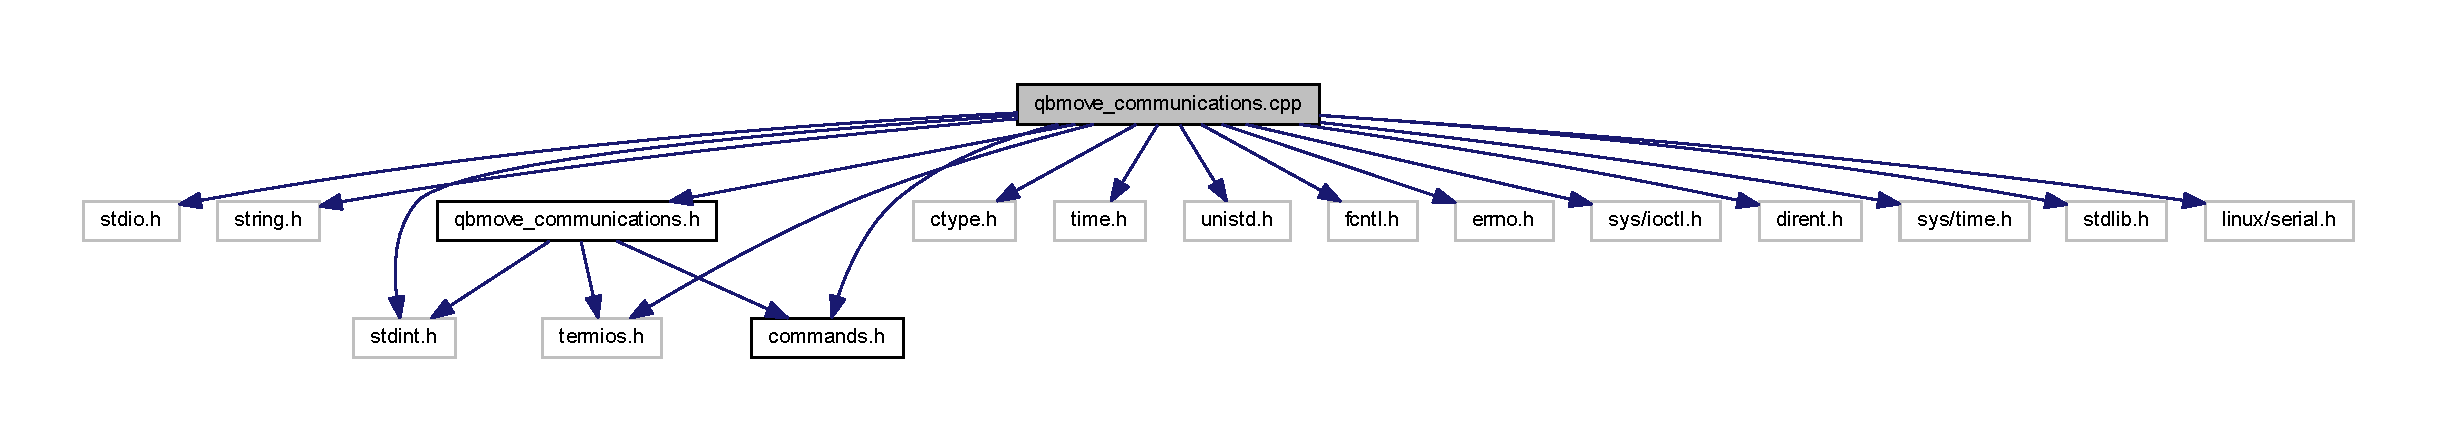
\includegraphics[width=350pt]{qbmove__communications_8cpp__incl}
\end{center}
\end{figure}
\subsection*{Macros}
\begin{DoxyCompactItemize}
\item 
\mbox{\label{qbmove__communications_8cpp_a6b20d41d6252e9871430c242cb1a56e7}} 
\#define \textbf{ B\+U\+F\+F\+E\+R\+\_\+\+S\+I\+ZE}~500
\begin{DoxyCompactList}\small\item\em Size of buffers that store communication packets. \end{DoxyCompactList}\end{DoxyCompactItemize}


\subsection{Detailed Description}
Library of functions for serial port communication with a board. 

\begin{DoxyDate}{Date}
October 01, 2017 
\end{DoxyDate}
\begin{DoxyAuthor}{Author}
{\itshape Centro \char`\"{}\+E.\+Piaggio\char`\"{}} 
\end{DoxyAuthor}
\begin{DoxyCopyright}{Copyright}
(C) 2012-\/2016 qbrobotics. All rights reserved. 

(C) 2017 Centro \char`\"{}\+E.\+Piaggio\char`\"{}. All rights reserved.
\end{DoxyCopyright}
Check the \doxyref{qbmove\+\_\+communications.h}{p.}{qbmove__communications_8h} file for a complete description of the public functions implemented in \doxyref{qbmove\+\_\+communications.\+cpp}{p.}{qbmove__communications_8cpp}. 
\section{qbmove\+\_\+communications.\+h File Reference}
\label{qbmove__communications_8h}\index{qbmove\+\_\+communications.\+h@{qbmove\+\_\+communications.\+h}}


Library of functions for S\+E\+R\+I\+AL P\+O\+RT communication with a board. Function Prototypes.  


{\ttfamily \#include $<$termios.\+h$>$}\newline
{\ttfamily \#include \char`\"{}commands.\+h\char`\"{}}\newline
{\ttfamily \#include $<$stdint.\+h$>$}\newline
Include dependency graph for qbmove\+\_\+communications.\+h\+:
\nopagebreak
\begin{figure}[H]
\begin{center}
\leavevmode
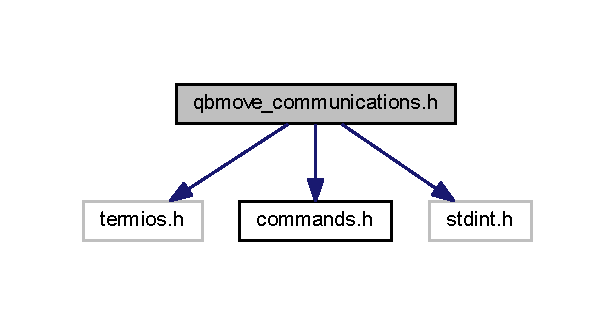
\includegraphics[width=295pt]{qbmove__communications_8h__incl}
\end{center}
\end{figure}
This graph shows which files directly or indirectly include this file\+:
\nopagebreak
\begin{figure}[H]
\begin{center}
\leavevmode
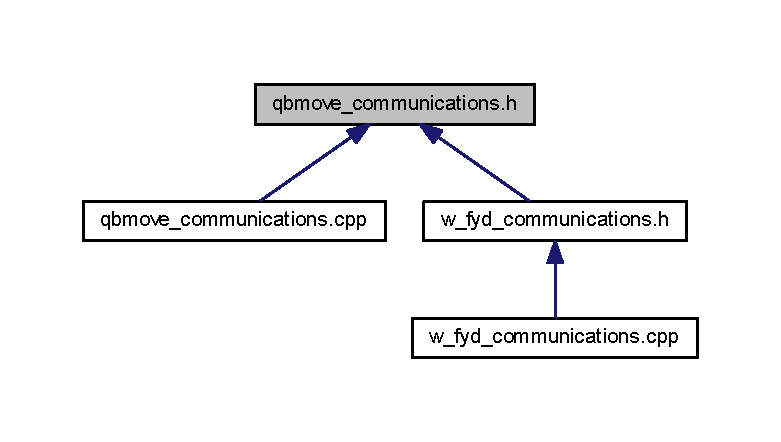
\includegraphics[width=350pt]{qbmove__communications_8h__dep__incl}
\end{center}
\end{figure}
\subsection*{Data Structures}
\begin{DoxyCompactItemize}
\item 
struct \textbf{ comm\+\_\+settings}
\end{DoxyCompactItemize}
\subsection*{Macros}
\begin{DoxyCompactItemize}
\item 
\mbox{\label{qbmove__communications_8h_ab521aa5010fb1afb801a899a55569e03}} 
\#define {\bfseries H\+A\+N\+D\+LE}~int
\item 
\mbox{\label{qbmove__communications_8h_a5fdc7facea201bfce4ad308105f88d0c}} 
\#define {\bfseries I\+N\+V\+A\+L\+I\+D\+\_\+\+H\+A\+N\+D\+L\+E\+\_\+\+V\+A\+L\+UE}~-\/1
\item 
\mbox{\label{qbmove__communications_8h_a44483e681594d0e510fd59c2b4b09ed9}} 
\#define {\bfseries B\+A\+U\+D\+\_\+\+R\+A\+T\+E\+\_\+\+T\+\_\+2000000}~0
\item 
\mbox{\label{qbmove__communications_8h_ad2c3e3edb0886633d686996e2f8c48e6}} 
\#define {\bfseries B\+A\+U\+D\+\_\+\+R\+A\+T\+E\+\_\+\+T\+\_\+460800}~1
\item 
\mbox{\label{qbmove__communications_8h_ab5b4465b1096182b9ebb03e87d572c59}} 
\#define {\bfseries M\+A\+X\+\_\+\+W\+A\+T\+C\+H\+D\+O\+G\+\_\+\+T\+I\+ME}~500
\item 
\mbox{\label{qbmove__communications_8h_a18e13c9ac88403c42395bb0af487eb2d}} 
\#define {\bfseries R\+E\+A\+D\+\_\+\+T\+I\+M\+E\+O\+UT}~4000
\end{DoxyCompactItemize}
\subsection*{Typedefs}
\begin{DoxyCompactItemize}
\item 
\mbox{\label{qbmove__communications_8h_a4a4b9cd04b7bc0361256581b13fadbdc}} 
typedef struct \textbf{ comm\+\_\+settings} {\bfseries comm\+\_\+settings}
\end{DoxyCompactItemize}
\subsection*{Functions}
\begin{Indent}\textbf{ Virtual C\+OM (R\+S485) functions}\par
\begin{DoxyCompactItemize}
\item 
int \textbf{ R\+S485list\+Ports} (char list\+\_\+of\+\_\+ports[10][255])
\item 
void \textbf{ open\+R\+S485} (\textbf{ comm\+\_\+settings} $\ast$comm\+\_\+settings\+\_\+t, const char $\ast$port\+\_\+s, int B\+A\+U\+D\+\_\+\+R\+A\+TE=B2000000)
\item 
void \textbf{ close\+R\+S485} (\textbf{ comm\+\_\+settings} $\ast$comm\+\_\+settings\+\_\+t)
\item 
int \textbf{ R\+S485read} (\textbf{ comm\+\_\+settings} $\ast$comm\+\_\+settings\+\_\+t, int id, char $\ast$package)
\item 
int \textbf{ R\+S485\+List\+Devices} (\textbf{ comm\+\_\+settings} $\ast$comm\+\_\+settings\+\_\+t, char list\+\_\+of\+\_\+ids[255])
\item 
void \textbf{ R\+S485\+Get\+Info} (\textbf{ comm\+\_\+settings} $\ast$comm\+\_\+settings\+\_\+t, char $\ast$buffer)
\end{DoxyCompactItemize}
\end{Indent}
\begin{Indent}\textbf{ qb\+A\+PI Commands}\par
\begin{DoxyCompactItemize}
\item 
int \textbf{ comm\+Ping} (\textbf{ comm\+\_\+settings} $\ast$comm\+\_\+settings\+\_\+t, int id)
\item 
void \textbf{ comm\+Activate} (\textbf{ comm\+\_\+settings} $\ast$comm\+\_\+settings\+\_\+t, int id, char activate)
\item 
void \textbf{ comm\+Set\+Baud\+Rate} (\textbf{ comm\+\_\+settings} $\ast$comm\+\_\+settings\+\_\+t, int id, short int baudrate)
\item 
void \textbf{ comm\+Set\+Watch\+Dog} (\textbf{ comm\+\_\+settings} $\ast$comm\+\_\+settings\+\_\+t, int id, short int wdt)
\item 
void \textbf{ comm\+Set\+Inputs} (\textbf{ comm\+\_\+settings} $\ast$comm\+\_\+settings\+\_\+t, int id, short int inputs[$\,$])
\item 
void \textbf{ comm\+Set\+Pos\+Stiff} (\textbf{ comm\+\_\+settings} $\ast$comm\+\_\+settings\+\_\+t, int id, short int inputs[$\,$])
\item 
int \textbf{ comm\+Get\+Inputs} (\textbf{ comm\+\_\+settings} $\ast$comm\+\_\+settings\+\_\+t, int id, short int inputs[2])
\item 
int \textbf{ comm\+Get\+Measurements} (\textbf{ comm\+\_\+settings} $\ast$comm\+\_\+settings\+\_\+t, int id, short int measurements[3])
\item 
int \textbf{ comm\+Get\+Counters} (\textbf{ comm\+\_\+settings} $\ast$comm\+\_\+settings\+\_\+t, int id, short unsigned int counters[20])
\item 
int \textbf{ comm\+Get\+Currents} (\textbf{ comm\+\_\+settings} $\ast$comm\+\_\+settings\+\_\+t, int id, short int currents[2])
\item 
int \textbf{ comm\+Get\+Curr\+And\+Meas} (\textbf{ comm\+\_\+settings} $\ast$comm\+\_\+settings\+\_\+t, int id, short int $\ast$values)
\item 
int \textbf{ comm\+Get\+Emg} (\textbf{ comm\+\_\+settings} $\ast$comm\+\_\+settings\+\_\+t, int id, short int emg[2])
\item 
int \textbf{ comm\+Get\+Velocities} (\textbf{ comm\+\_\+settings} $\ast$comm\+\_\+settings\+\_\+t, int id, short int measurements[$\,$])
\item 
int \textbf{ comm\+Get\+Accelerations} (\textbf{ comm\+\_\+settings} $\ast$comm\+\_\+settings\+\_\+t, int id, short int measurements[$\,$])
\item 
int \textbf{ comm\+Get\+Activate} (\textbf{ comm\+\_\+settings} $\ast$comm\+\_\+settings\+\_\+t, int id, char $\ast$activate)
\item 
int \textbf{ comm\+Get\+Info} (\textbf{ comm\+\_\+settings} $\ast$comm\+\_\+settings\+\_\+t, int id, short int info\+\_\+type, char $\ast$info)
\item 
int \textbf{ comm\+Bootloader} (\textbf{ comm\+\_\+settings} $\ast$comm\+\_\+settings\+\_\+t, int id)
\item 
int \textbf{ comm\+Calibrate} (\textbf{ comm\+\_\+settings} $\ast$comm\+\_\+settings\+\_\+t, int id)
\item 
int \textbf{ comm\+Hand\+Calibrate} (\textbf{ comm\+\_\+settings} $\ast$comm\+\_\+settings\+\_\+t, int id, short int speed, short int repetitions)
\end{DoxyCompactItemize}
\end{Indent}
\begin{Indent}\textbf{ qb\+A\+PI Parameters}\par
\begin{DoxyCompactItemize}
\item 
int \textbf{ comm\+Set\+Zeros} (\textbf{ comm\+\_\+settings} $\ast$comm\+\_\+settings\+\_\+t, int id, void $\ast$values, unsigned short num\+\_\+of\+\_\+values)
\item 
int \textbf{ comm\+Get\+Param\+List} (\textbf{ comm\+\_\+settings} $\ast$comm\+\_\+settings\+\_\+t, int id, unsigned short index, void $\ast$values, unsigned short value\+\_\+size, unsigned short num\+\_\+of\+\_\+values, uint8\+\_\+t $\ast$buffer)
\item 
int \textbf{ comm\+Store\+Params} (\textbf{ comm\+\_\+settings} $\ast$comm\+\_\+settings\+\_\+t, int id)
\item 
int \textbf{ comm\+Store\+Default\+Params} (\textbf{ comm\+\_\+settings} $\ast$comm\+\_\+settings\+\_\+t, int id)
\item 
int \textbf{ comm\+Restore\+Params} (\textbf{ comm\+\_\+settings} $\ast$comm\+\_\+settings\+\_\+t, int id)
\item 
int \textbf{ comm\+Init\+Mem} (\textbf{ comm\+\_\+settings} $\ast$comm\+\_\+settings\+\_\+t, int id)
\end{DoxyCompactItemize}
\end{Indent}
\begin{Indent}\textbf{ General Functions}\par
\begin{DoxyCompactItemize}
\item 
long \textbf{ timevaldiff} (struct timeval $\ast$starttime, struct timeval $\ast$finishtime)
\item 
char \textbf{ checksum} (char $\ast$data\+\_\+buffer, int data\+\_\+length)
\end{DoxyCompactItemize}
\end{Indent}
\begin{Indent}\textbf{ Functions for other devices}\par
\begin{DoxyCompactItemize}
\item 
int \textbf{ comm\+Ext\+Drive} (\textbf{ comm\+\_\+settings} $\ast$comm\+\_\+settings\+\_\+t, int id, char ext\+\_\+input)
\item 
void \textbf{ comm\+Set\+Cuff\+Inputs} (\textbf{ comm\+\_\+settings} $\ast$comm\+\_\+settings\+\_\+t, int id, int flag)
\item 
int \textbf{ comm\+Get\+Joystick} (\textbf{ comm\+\_\+settings} $\ast$comm\+\_\+settings\+\_\+t, int id, short int joystick[2])
\end{DoxyCompactItemize}
\end{Indent}


\subsection{Detailed Description}
Library of functions for S\+E\+R\+I\+AL P\+O\+RT communication with a board. Function Prototypes. 

\begin{DoxyDate}{Date}
October 01, 2017 
\end{DoxyDate}
\begin{DoxyAuthor}{Author}
{\itshape Centro \char`\"{}\+E.\+Piaggio\char`\"{}} 
\end{DoxyAuthor}
\begin{DoxyCopyright}{Copyright}
(C) 2012-\/2016 qbrobotics. All rights reserved. 

(C) 2017 Centro \char`\"{}\+E.\+Piaggio\char`\"{}. All rights reserved.
\end{DoxyCopyright}
This library contains all necessary functions for communicating with a board when using a U\+SB to R\+S485 connector that provides a Virtual C\+OM interface. 

\subsection{Function Documentation}
\mbox{\label{qbmove__communications_8h_a35819265b74001583803a2295b3236dc}} 
\index{qbmove\+\_\+communications.\+h@{qbmove\+\_\+communications.\+h}!checksum@{checksum}}
\index{checksum@{checksum}!qbmove\+\_\+communications.\+h@{qbmove\+\_\+communications.\+h}}
\subsubsection{checksum()}
{\footnotesize\ttfamily char checksum (\begin{DoxyParamCaption}\item[{char $\ast$}]{data\+\_\+buffer,  }\item[{int}]{data\+\_\+length }\end{DoxyParamCaption})}

This functions returns an 8 bit L\+CR checksum over the lenght of a buffer.


\begin{DoxyParams}{Parameters}
{\em data\+\_\+buffer} & Buffer. \\
\hline
{\em data\+\_\+length} & Buffer length.\\
\hline
\end{DoxyParams}
\begin{DoxyParagraph}{Example}

\begin{DoxyCode}
\textcolor{keywordtype}{char}    aux;
\textcolor{keywordtype}{char}    buffer[5];

buffer  = \textcolor{stringliteral}{"abcde"};
aux     = checksum(buffer,5);
printf(\textcolor{stringliteral}{"Checksum: %d"}, (\textcolor{keywordtype}{int}) aux)
\end{DoxyCode}
 
\end{DoxyParagraph}
\mbox{\label{qbmove__communications_8h_a5f87643fab51e02e4eab71bf4ab1a33a}} 
\index{qbmove\+\_\+communications.\+h@{qbmove\+\_\+communications.\+h}!close\+R\+S485@{close\+R\+S485}}
\index{close\+R\+S485@{close\+R\+S485}!qbmove\+\_\+communications.\+h@{qbmove\+\_\+communications.\+h}}
\subsubsection{close\+R\+S485()}
{\footnotesize\ttfamily void close\+R\+S485 (\begin{DoxyParamCaption}\item[{\textbf{ comm\+\_\+settings} $\ast$}]{comm\+\_\+settings\+\_\+t }\end{DoxyParamCaption})}

This function is used to close a serial port being used with the qb\+Move or an qb\+Hand.


\begin{DoxyParams}{Parameters}
{\em comm\+\_\+settings\+\_\+t} & A {\itshape \doxyref{comm\+\_\+settings}{p.}{structcomm__settings}} structure containing info about the communication settings.\\
\hline
\end{DoxyParams}
\begin{DoxyParagraph}{Example}

\begin{DoxyCode}
comm_settings   comm\_settings\_t;

openRS485(&comm\_settings\_t,\textcolor{stringliteral}{"/dev/tty.usbserial-128"});
closeRS485(&comm\_settings\_t);
\end{DoxyCode}
 
\end{DoxyParagraph}
\mbox{\label{qbmove__communications_8h_aff081c6687d87e38cddfe714ad2de0fd}} 
\index{qbmove\+\_\+communications.\+h@{qbmove\+\_\+communications.\+h}!comm\+Activate@{comm\+Activate}}
\index{comm\+Activate@{comm\+Activate}!qbmove\+\_\+communications.\+h@{qbmove\+\_\+communications.\+h}}
\subsubsection{comm\+Activate()}
{\footnotesize\ttfamily void comm\+Activate (\begin{DoxyParamCaption}\item[{\textbf{ comm\+\_\+settings} $\ast$}]{comm\+\_\+settings\+\_\+t,  }\item[{int}]{id,  }\item[{char}]{activate }\end{DoxyParamCaption})}

This function activates or deactivates a qb\+Move or a qb\+Hand connected to the serial port.


\begin{DoxyParams}{Parameters}
{\em comm\+\_\+settings\+\_\+t} & A {\itshape \doxyref{comm\+\_\+settings}{p.}{structcomm__settings}} structure containing info about the communication settings.\\
\hline
{\em id} & The device\textquotesingle{}s id number. \\
\hline
{\em activate} & T\+R\+UE to turn motors on. F\+A\+L\+SE to turn motors off. \\
\hline
\end{DoxyParams}
\begin{DoxyParagraph}{Example}

\begin{DoxyCode}
comm_settings   comm\_settings\_t;
\textcolor{keywordtype}{int}             device\_id = 65;

openRS485(&comm\_settings\_t,\textcolor{stringliteral}{"/dev/tty.usbserial-128"});
commActivate(&comm\_settings\_t, device\_id, TRUE);
closeRS485(&comm\_settings\_t);
\end{DoxyCode}
 
\end{DoxyParagraph}
\mbox{\label{qbmove__communications_8h_a70990e1cf4d18b3baeb3c7295dbd6426}} 
\index{qbmove\+\_\+communications.\+h@{qbmove\+\_\+communications.\+h}!comm\+Bootloader@{comm\+Bootloader}}
\index{comm\+Bootloader@{comm\+Bootloader}!qbmove\+\_\+communications.\+h@{qbmove\+\_\+communications.\+h}}
\subsubsection{comm\+Bootloader()}
{\footnotesize\ttfamily int comm\+Bootloader (\begin{DoxyParamCaption}\item[{\textbf{ comm\+\_\+settings} $\ast$}]{comm\+\_\+settings\+\_\+t,  }\item[{int}]{id }\end{DoxyParamCaption})}

This function sends the board in bootloader modality in order to update the firmware on the board


\begin{DoxyParams}{Parameters}
{\em comm\+\_\+settings\+\_\+t} & A {\itshape \doxyref{comm\+\_\+settings}{p.}{structcomm__settings}} structure containing info about the communication settings.\\
\hline
{\em id} & The device\textquotesingle{}s id number.\\
\hline
\end{DoxyParams}
\begin{DoxyReturn}{Returns}
Return 0 on success, -\/1 otherwise
\end{DoxyReturn}
\begin{DoxyParagraph}{Example}

\begin{DoxyCode}
comm_settings comm\_settings\_t;
\textcolor{keywordtype}{int}     device\_id = 65;

openRS485(&comm\_settings\_t,\textcolor{stringliteral}{"/dev/tty.usbserial-128"});
commBootloader(&comm\_settings\_t, device\_id);
closeRS485(&comm\_settings\_t);
\end{DoxyCode}
 
\end{DoxyParagraph}
\mbox{\label{qbmove__communications_8h_a92ef5f590c59ab49a224b8e612eb08ac}} 
\index{qbmove\+\_\+communications.\+h@{qbmove\+\_\+communications.\+h}!comm\+Calibrate@{comm\+Calibrate}}
\index{comm\+Calibrate@{comm\+Calibrate}!qbmove\+\_\+communications.\+h@{qbmove\+\_\+communications.\+h}}
\subsubsection{comm\+Calibrate()}
{\footnotesize\ttfamily int comm\+Calibrate (\begin{DoxyParamCaption}\item[{\textbf{ comm\+\_\+settings} $\ast$}]{comm\+\_\+settings\+\_\+t,  }\item[{int}]{id }\end{DoxyParamCaption})}

This function is used to calibrate the maximum stiffness value of the qb\+Move


\begin{DoxyParams}{Parameters}
{\em comm\+\_\+settings\+\_\+t} & A {\itshape \doxyref{comm\+\_\+settings}{p.}{structcomm__settings}} structure containing info about the communication settings.\\
\hline
{\em id} & The device\textquotesingle{}s id number.\\
\hline
\end{DoxyParams}
\begin{DoxyReturn}{Returns}
Returns 0 on success, -\/1 otherwise
\end{DoxyReturn}
\begin{DoxyParagraph}{Example}

\begin{DoxyCode}
comm_settings comm\_settings\_t;
\textcolor{keywordtype}{int}     device\_id = 65;

openRS485(&comm\_settings\_t,\textcolor{stringliteral}{"/dev/tty.usbserial-128"});
commCalibrate(&comm\_settings\_t, device\_id);
closeRS485(&comm\_settings\_t);
\end{DoxyCode}
 
\end{DoxyParagraph}
\mbox{\label{qbmove__communications_8h_ac9705be6201442447bfa37e498721d2b}} 
\index{qbmove\+\_\+communications.\+h@{qbmove\+\_\+communications.\+h}!comm\+Ext\+Drive@{comm\+Ext\+Drive}}
\index{comm\+Ext\+Drive@{comm\+Ext\+Drive}!qbmove\+\_\+communications.\+h@{qbmove\+\_\+communications.\+h}}
\subsubsection{comm\+Ext\+Drive()}
{\footnotesize\ttfamily int comm\+Ext\+Drive (\begin{DoxyParamCaption}\item[{\textbf{ comm\+\_\+settings} $\ast$}]{comm\+\_\+settings\+\_\+t,  }\item[{int}]{id,  }\item[{char}]{ext\+\_\+input }\end{DoxyParamCaption})}

This function is used with the armslider device. Is used to drive another board with the inputs of the first one


\begin{DoxyParams}{Parameters}
{\em comm\+\_\+settings\+\_\+t} & A {\itshape \doxyref{comm\+\_\+settings}{p.}{structcomm__settings}} structure containing info about the comunication settings. \\
\hline
{\em id} & The id of the board drive. \\
\hline
{\em ext\+\_\+input} & A flag used to activate the external drive functionality of the board.\\
\hline
\end{DoxyParams}
\begin{DoxyReturn}{Returns}
A negative value if something went wrong, a zero if everything went fine. 
\end{DoxyReturn}
\mbox{\label{qbmove__communications_8h_abfa23acd4ac72099fa96a32df01969d2}} 
\index{qbmove\+\_\+communications.\+h@{qbmove\+\_\+communications.\+h}!comm\+Get\+Accelerations@{comm\+Get\+Accelerations}}
\index{comm\+Get\+Accelerations@{comm\+Get\+Accelerations}!qbmove\+\_\+communications.\+h@{qbmove\+\_\+communications.\+h}}
\subsubsection{comm\+Get\+Accelerations()}
{\footnotesize\ttfamily int comm\+Get\+Accelerations (\begin{DoxyParamCaption}\item[{\textbf{ comm\+\_\+settings} $\ast$}]{comm\+\_\+settings\+\_\+t,  }\item[{int}]{id,  }\item[{short int}]{measurements[$\,$] }\end{DoxyParamCaption})}

This function gets the acceleration of the qb\+Hand motor


\begin{DoxyParams}{Parameters}
{\em comm\+\_\+settings\+\_\+t} & A {\itshape \doxyref{comm\+\_\+settings}{p.}{structcomm__settings}} structure containing info about the communication settings.\\
\hline
{\em id} & The device\textquotesingle{}s id number. \\
\hline
{\em measurements} & Velocity measurements.\\
\hline
\end{DoxyParams}
\begin{DoxyReturn}{Returns}
Returns 0 if communication was ok, -\/1 otherwise.
\end{DoxyReturn}
\begin{DoxyParagraph}{Example}

\begin{DoxyCode}
comm_settings    comm\_settings\_t;
\textcolor{keywordtype}{int}              device\_id = 65;
\textcolor{keywordtype}{short} \textcolor{keywordtype}{int}        acc\_measurements[3];

openRS485(&comm\_settings\_t,\textcolor{stringliteral}{"/dev/tty.usbserial-128"});

\textcolor{keywordflow}{if}(!commGetAccelerations(&comm\_settings\_t, device\_id, acc\_measurements))
    printf(\textcolor{stringliteral}{"Measurements: %d\(\backslash\)t%d\(\backslash\)t%d\(\backslash\)n"}, acc\_measurements[0], acc\_measurements[1], acc\_measurements[2]);
\textcolor{keywordflow}{else}
    puts(\textcolor{stringliteral}{"Couldn't retrieve accelerations."});

closeRS485(&comm\_settings\_t);
\end{DoxyCode}
 
\end{DoxyParagraph}
\mbox{\label{qbmove__communications_8h_abaec903aef1ce3cebb5f42f63995c2e1}} 
\index{qbmove\+\_\+communications.\+h@{qbmove\+\_\+communications.\+h}!comm\+Get\+Activate@{comm\+Get\+Activate}}
\index{comm\+Get\+Activate@{comm\+Get\+Activate}!qbmove\+\_\+communications.\+h@{qbmove\+\_\+communications.\+h}}
\subsubsection{comm\+Get\+Activate()}
{\footnotesize\ttfamily int comm\+Get\+Activate (\begin{DoxyParamCaption}\item[{\textbf{ comm\+\_\+settings} $\ast$}]{comm\+\_\+settings\+\_\+t,  }\item[{int}]{id,  }\item[{char $\ast$}]{activate }\end{DoxyParamCaption})}

This function gets the activation status of a qb\+Move or a qb\+Hand connected to the serial port.


\begin{DoxyParams}{Parameters}
{\em comm\+\_\+settings\+\_\+t} & A {\itshape \doxyref{comm\+\_\+settings}{p.}{structcomm__settings}} structure containing info about the communication settings.\\
\hline
{\em id} & The device\textquotesingle{}s id number. \\
\hline
{\em activation} & Activation status.\\
\hline
\end{DoxyParams}
\begin{DoxyReturn}{Returns}
Returns 0 if communication was ok, -\/1 otherwise.
\end{DoxyReturn}
\begin{DoxyParagraph}{Example}

\begin{DoxyCode}
comm_settings comm\_settings\_t;
\textcolor{keywordtype}{int}     device\_id = 65;
\textcolor{keywordtype}{char}    activation\_status;

openRS485(&comm\_settings\_t,\textcolor{stringliteral}{"/dev/tty.usbserial-128"});

\textcolor{keywordflow}{if}(!commGetActivate(&comm\_settings\_t, DEVICE\_ID, activation\_status))
    printf(\textcolor{stringliteral}{"Activation status: %d\(\backslash\)n"}, &activation\_status);
\textcolor{keywordflow}{else}
    puts(\textcolor{stringliteral}{"Couldn't retrieve activation status."});

closeRS485(&comm\_settings\_t);
\end{DoxyCode}
 
\end{DoxyParagraph}
\mbox{\label{qbmove__communications_8h_aab579187b08cac507c18584b242eb02d}} 
\index{qbmove\+\_\+communications.\+h@{qbmove\+\_\+communications.\+h}!comm\+Get\+Counters@{comm\+Get\+Counters}}
\index{comm\+Get\+Counters@{comm\+Get\+Counters}!qbmove\+\_\+communications.\+h@{qbmove\+\_\+communications.\+h}}
\subsubsection{comm\+Get\+Counters()}
{\footnotesize\ttfamily int comm\+Get\+Counters (\begin{DoxyParamCaption}\item[{\textbf{ comm\+\_\+settings} $\ast$}]{comm\+\_\+settings\+\_\+t,  }\item[{int}]{id,  }\item[{short unsigned int}]{counters[20] }\end{DoxyParamCaption})}

This function gets counters values from a qb\+Move connected to the serial port.


\begin{DoxyParams}{Parameters}
{\em comm\+\_\+settings\+\_\+t} & A {\itshape \doxyref{comm\+\_\+settings}{p.}{structcomm__settings}} structure containing info about the communication settings.\\
\hline
{\em id} & The device\textquotesingle{}s id number. \\
\hline
{\em counters} & Counters\\
\hline
\end{DoxyParams}
\begin{DoxyReturn}{Returns}
Returns 0 if communication was ok, -\/1 otherwise.
\end{DoxyReturn}
\begin{DoxyParagraph}{Example}

\begin{DoxyCode}
comm_settings       comm\_settings\_t;
\textcolor{keywordtype}{int}                 device\_id = 65;
\textcolor{keywordtype}{short} \textcolor{keywordtype}{unsigned} \textcolor{keywordtype}{int}  counters[20];

openRS485(&comm\_settings\_t,\textcolor{stringliteral}{"/dev/tty.usbserial-128"});

\textcolor{keywordflow}{if}(!commGetCounters(&comm\_settings\_t, DEVICE\_ID, counters))
    printf(\textcolor{stringliteral}{"Counters: %d\(\backslash\)t%d\(\backslash\)t \{...\} %d\(\backslash\)n"}, counters[0], counters[1], \{...\}, counters[20]);
\textcolor{keywordflow}{else}
    puts(\textcolor{stringliteral}{"Couldn't retrieve counters."});

closeRS485(&comm\_settings\_t);
\end{DoxyCode}
 
\end{DoxyParagraph}
\mbox{\label{qbmove__communications_8h_a3f700c3fc90215428707c7c98b3d538f}} 
\index{qbmove\+\_\+communications.\+h@{qbmove\+\_\+communications.\+h}!comm\+Get\+Curr\+And\+Meas@{comm\+Get\+Curr\+And\+Meas}}
\index{comm\+Get\+Curr\+And\+Meas@{comm\+Get\+Curr\+And\+Meas}!qbmove\+\_\+communications.\+h@{qbmove\+\_\+communications.\+h}}
\subsubsection{comm\+Get\+Curr\+And\+Meas()}
{\footnotesize\ttfamily int comm\+Get\+Curr\+And\+Meas (\begin{DoxyParamCaption}\item[{\textbf{ comm\+\_\+settings} $\ast$}]{comm\+\_\+settings\+\_\+t,  }\item[{int}]{id,  }\item[{short int $\ast$}]{values }\end{DoxyParamCaption})}

This function gets currents and position measurements from a qb\+Move or a qb\+Hand connected to the serial port


\begin{DoxyParams}{Parameters}
{\em comm\+\_\+settings\+\_\+t} & A {\itshape \doxyref{comm\+\_\+settings}{p.}{structcomm__settings}} structure containing info about the communication settings.\\
\hline
{\em id} & The device\textquotesingle{}s id number. \\
\hline
{\em values} & Current and position measurements. Currents are in first two positions\\
\hline
\end{DoxyParams}
\begin{DoxyReturn}{Returns}
Returns 0 if communication was ok, -\/1 otherwise.
\end{DoxyReturn}
\begin{DoxyParagraph}{Example}

\begin{DoxyCode}
comm_settings    comm\_settings\_t;
\textcolor{keywordtype}{int}              device\_id = 65;
\textcolor{keywordtype}{short} \textcolor{keywordtype}{int}        values[5];

openRS485(&comm\_settings\_t,\textcolor{stringliteral}{"/dev/tty.usbserial-128"});

 \textcolor{keywordflow}{if}(!commGetCurrAndMeas(&comm\_settings\_t, device\_id, currents))\{
     printf(\textcolor{stringliteral}{"Currents: %d\(\backslash\)t%d\(\backslash\)t%d\(\backslash\)n"},values[0], values[1]);
     printf(\textcolor{stringliteral}{"Measurements: %d\(\backslash\)t%d\(\backslash\)t%d\(\backslash\)n"}, values[2], values[3], values[4]);
 \}
 \textcolor{keywordflow}{else}
     puts(\textcolor{stringliteral}{"Couldn't retrieve currents."});

closeRS485(&comm\_settings\_t);
\end{DoxyCode}
 
\end{DoxyParagraph}
\mbox{\label{qbmove__communications_8h_a4b3c724150046fc4a766db52fa086fdf}} 
\index{qbmove\+\_\+communications.\+h@{qbmove\+\_\+communications.\+h}!comm\+Get\+Currents@{comm\+Get\+Currents}}
\index{comm\+Get\+Currents@{comm\+Get\+Currents}!qbmove\+\_\+communications.\+h@{qbmove\+\_\+communications.\+h}}
\subsubsection{comm\+Get\+Currents()}
{\footnotesize\ttfamily int comm\+Get\+Currents (\begin{DoxyParamCaption}\item[{\textbf{ comm\+\_\+settings} $\ast$}]{comm\+\_\+settings\+\_\+t,  }\item[{int}]{id,  }\item[{short int}]{currents[2] }\end{DoxyParamCaption})}

This function gets currents from a qb\+Move or a qb\+Hand connected to the serial port.


\begin{DoxyParams}{Parameters}
{\em comm\+\_\+settings\+\_\+t} & A {\itshape \doxyref{comm\+\_\+settings}{p.}{structcomm__settings}} structure containing info about the communication settings.\\
\hline
{\em id} & The device\textquotesingle{}s id number. \\
\hline
{\em currents} & Currents.\\
\hline
\end{DoxyParams}
\begin{DoxyReturn}{Returns}
Returns 0 if communication was ok, -\/1 otherwise.
\end{DoxyReturn}
\begin{DoxyParagraph}{Example}

\begin{DoxyCode}
comm_settings    comm\_settings\_t;
\textcolor{keywordtype}{int}              device\_id = 65;
\textcolor{keywordtype}{short} \textcolor{keywordtype}{int}        currents[2];

openRS485(&comm\_settings\_t,\textcolor{stringliteral}{"/dev/tty.usbserial-128"});

\textcolor{keywordflow}{if}(!commGetCurrents(&comm\_settings\_t, device\_id, currents))
    printf(\textcolor{stringliteral}{"Measurements: %d\(\backslash\)t%d\(\backslash\)t%d\(\backslash\)n"},currents[0], currents[1]);
\textcolor{keywordflow}{else}
    puts(\textcolor{stringliteral}{"Couldn't retrieve currents."});

closeRS485(&comm\_settings\_t);
\end{DoxyCode}
 
\end{DoxyParagraph}
\mbox{\label{qbmove__communications_8h_a731e861c53a68c7e2e57d36383bf3360}} 
\index{qbmove\+\_\+communications.\+h@{qbmove\+\_\+communications.\+h}!comm\+Get\+Emg@{comm\+Get\+Emg}}
\index{comm\+Get\+Emg@{comm\+Get\+Emg}!qbmove\+\_\+communications.\+h@{qbmove\+\_\+communications.\+h}}
\subsubsection{comm\+Get\+Emg()}
{\footnotesize\ttfamily int comm\+Get\+Emg (\begin{DoxyParamCaption}\item[{\textbf{ comm\+\_\+settings} $\ast$}]{comm\+\_\+settings\+\_\+t,  }\item[{int}]{id,  }\item[{short int}]{emg[2] }\end{DoxyParamCaption})}

This function gets measurements from electomyographics sensors connected to the qb\+Hand. IS U\+S\+ED O\+N\+LY W\+H\+EN T\+HE B\+O\+A\+RD IS U\+S\+ED F\+OR A Q\+B\+H\+A\+ND


\begin{DoxyParams}{Parameters}
{\em comm\+\_\+settings\+\_\+t} & A {\itshape \doxyref{comm\+\_\+settings}{p.}{structcomm__settings}} structure containing info about the communication settings.\\
\hline
{\em id} & The device\textquotesingle{}s id number. \\
\hline
{\em values} & Emg sensors measurements.\\
\hline
\end{DoxyParams}
\begin{DoxyReturn}{Returns}
Returns 0 if communication was ok, -\/1 otherwise.
\end{DoxyReturn}
\begin{DoxyParagraph}{Example}

\begin{DoxyCode}
comm_settings    comm\_settings\_t;
\textcolor{keywordtype}{int}              device\_id = 65;
\textcolor{keywordtype}{short} \textcolor{keywordtype}{int}        values[2];

openRS485(&comm\_settings\_t,\textcolor{stringliteral}{"/dev/tty.usbserial-128"});

\textcolor{keywordflow}{if}(!commGetEmg(&comm\_settings\_t, device\_id, values));
    printf(\textcolor{stringliteral}{"Measurements: %d\(\backslash\)t%d\(\backslash\)t%d\(\backslash\)n"}, values[0], values[1]);
\textcolor{keywordflow}{else}
    puts(\textcolor{stringliteral}{"Couldn't retrieve emg values."});

closeRS485(&comm\_settings\_t);
\end{DoxyCode}
 
\end{DoxyParagraph}
\mbox{\label{qbmove__communications_8h_a052291b3dd75dee6a33242268a1de657}} 
\index{qbmove\+\_\+communications.\+h@{qbmove\+\_\+communications.\+h}!comm\+Get\+Info@{comm\+Get\+Info}}
\index{comm\+Get\+Info@{comm\+Get\+Info}!qbmove\+\_\+communications.\+h@{qbmove\+\_\+communications.\+h}}
\subsubsection{comm\+Get\+Info()}
{\footnotesize\ttfamily int comm\+Get\+Info (\begin{DoxyParamCaption}\item[{\textbf{ comm\+\_\+settings} $\ast$}]{comm\+\_\+settings\+\_\+t,  }\item[{int}]{id,  }\item[{short int}]{info\+\_\+type,  }\item[{char $\ast$}]{info }\end{DoxyParamCaption})}

This function is used to ping the qb\+Move or the qb\+Hand and get information about the device.


\begin{DoxyParams}{Parameters}
{\em comm\+\_\+settings\+\_\+t} & A {\itshape \doxyref{comm\+\_\+settings}{p.}{structcomm__settings}} structure containing info about the communication settings.\\
\hline
{\em id} & The device\textquotesingle{}s id number. \\
\hline
{\em buffer} & Buffer that stores a string with information about the device. B\+U\+F\+F\+ER S\+I\+ZE M\+U\+ST BE AT L\+E\+A\+ST 500. \\
\hline
{\em info\+\_\+type} & Information to be retrieved.\\
\hline
\end{DoxyParams}
\begin{DoxyParagraph}{Example}

\begin{DoxyCode}
comm_settings comm\_settings\_t;
\textcolor{keywordtype}{char}    auxstring[500];
\textcolor{keywordtype}{int}     device\_id = 65;

openRS485(&comm\_settings\_t,\textcolor{stringliteral}{"/dev/tty.usbserial-128"});
commGetInfo(&comm\_settings\_t, device\_id, INFO_ALL, auxstring);
puts(auxstring);
closeRS485(&comm\_settings\_t);
\end{DoxyCode}
 
\end{DoxyParagraph}
\mbox{\label{qbmove__communications_8h_ae0a38427212fc15a1021d2459a86f2c0}} 
\index{qbmove\+\_\+communications.\+h@{qbmove\+\_\+communications.\+h}!comm\+Get\+Inputs@{comm\+Get\+Inputs}}
\index{comm\+Get\+Inputs@{comm\+Get\+Inputs}!qbmove\+\_\+communications.\+h@{qbmove\+\_\+communications.\+h}}
\subsubsection{comm\+Get\+Inputs()}
{\footnotesize\ttfamily int comm\+Get\+Inputs (\begin{DoxyParamCaption}\item[{\textbf{ comm\+\_\+settings} $\ast$}]{comm\+\_\+settings\+\_\+t,  }\item[{int}]{id,  }\item[{short int}]{inputs[2] }\end{DoxyParamCaption})}

This function gets input references from a qb\+Move or a qb\+Hand connected to the serial port.


\begin{DoxyParams}{Parameters}
{\em comm\+\_\+settings\+\_\+t} & A {\itshape \doxyref{comm\+\_\+settings}{p.}{structcomm__settings}} structure containing info about the communication settings.\\
\hline
{\em id} & The device\textquotesingle{}s id number. \\
\hline
{\em inputs} & Input references.\\
\hline
\end{DoxyParams}
\begin{DoxyReturn}{Returns}
Returns 0 if communication was ok, -\/1 otherwise.
\end{DoxyReturn}
\begin{DoxyParagraph}{Example}

\begin{DoxyCode}
comm_settings   comm\_settings\_t;
\textcolor{keywordtype}{int}             device\_id = 65;
\textcolor{keywordtype}{short} \textcolor{keywordtype}{int}       inputs[2];

openRS485(&comm\_settings\_t,\textcolor{stringliteral}{"/dev/tty.usbserial-128"});

\textcolor{keywordflow}{if}(!commGetInputs(&comm\_settings\_t, DEVICE\_ID, inputs))
    printf(\textcolor{stringliteral}{"Inputs: %d\(\backslash\)t%d\(\backslash\)n"},inputs[0], inputs[1]);
\textcolor{keywordflow}{else}
    puts(\textcolor{stringliteral}{"Couldn't retrieve device inputs."});

closeRS485(&comm\_settings\_t);
\end{DoxyCode}
 
\end{DoxyParagraph}
\mbox{\label{qbmove__communications_8h_af78c08053431bb4d516f9ec49b651280}} 
\index{qbmove\+\_\+communications.\+h@{qbmove\+\_\+communications.\+h}!comm\+Get\+Joystick@{comm\+Get\+Joystick}}
\index{comm\+Get\+Joystick@{comm\+Get\+Joystick}!qbmove\+\_\+communications.\+h@{qbmove\+\_\+communications.\+h}}
\subsubsection{comm\+Get\+Joystick()}
{\footnotesize\ttfamily int comm\+Get\+Joystick (\begin{DoxyParamCaption}\item[{\textbf{ comm\+\_\+settings} $\ast$}]{comm\+\_\+settings\+\_\+t,  }\item[{int}]{id,  }\item[{short int}]{joystick[2] }\end{DoxyParamCaption})}

This function gets joystick measurementes from a softhand connected to the serial port.


\begin{DoxyParams}{Parameters}
{\em comm\+\_\+settings\+\_\+t} & A {\itshape \doxyref{comm\+\_\+settings}{p.}{structcomm__settings}} structure containing info about the communication settings.\\
\hline
{\em id} & The device\textquotesingle{}s id number. \\
\hline
{\em joystick} & Joystick analog measurements.\\
\hline
\end{DoxyParams}
\begin{DoxyReturn}{Returns}
Returns 0 if communication was ok, -\/1 otherwise.
\end{DoxyReturn}
\begin{DoxyParagraph}{Example}

\begin{DoxyCode}
comm_settings    comm\_settings\_t;
\textcolor{keywordtype}{int}              device\_id = 65;
\textcolor{keywordtype}{short} \textcolor{keywordtype}{int}        joystick[2];

openRS485(&comm\_settings\_t,\textcolor{stringliteral}{"/dev/tty.usbserial-128"});

\textcolor{keywordflow}{if}(!commGetJoystick(&comm\_settings\_t, device\_id, joystick))
    printf(\textcolor{stringliteral}{"Measurements: %d\(\backslash\)t%d\(\backslash\)t%d\(\backslash\)n"},joystick[0], joystick[1]);
\textcolor{keywordflow}{else}
    puts(\textcolor{stringliteral}{"Couldn't retrieve joystick measurements."});

closeRS485(&comm\_settings\_t);
\end{DoxyCode}
 
\end{DoxyParagraph}
\mbox{\label{qbmove__communications_8h_a06a73f0c93c7ae12a95541c1feee10b7}} 
\index{qbmove\+\_\+communications.\+h@{qbmove\+\_\+communications.\+h}!comm\+Get\+Measurements@{comm\+Get\+Measurements}}
\index{comm\+Get\+Measurements@{comm\+Get\+Measurements}!qbmove\+\_\+communications.\+h@{qbmove\+\_\+communications.\+h}}
\subsubsection{comm\+Get\+Measurements()}
{\footnotesize\ttfamily int comm\+Get\+Measurements (\begin{DoxyParamCaption}\item[{\textbf{ comm\+\_\+settings} $\ast$}]{comm\+\_\+settings\+\_\+t,  }\item[{int}]{id,  }\item[{short int}]{measurements[3] }\end{DoxyParamCaption})}

This function gets position measurements from a qb\+Move or a qb\+Hand connected to the serial port.


\begin{DoxyParams}{Parameters}
{\em comm\+\_\+settings\+\_\+t} & A {\itshape \doxyref{comm\+\_\+settings}{p.}{structcomm__settings}} structure containing info about the communication settings.\\
\hline
{\em id} & The device\textquotesingle{}s id number. \\
\hline
{\em measurements} & Measurements.\\
\hline
\end{DoxyParams}
\begin{DoxyReturn}{Returns}
Returns 0 if communication was ok, -\/1 otherwise.
\end{DoxyReturn}
\begin{DoxyParagraph}{Example}

\begin{DoxyCode}
comm_settings   comm\_settings\_t;
\textcolor{keywordtype}{int}             device\_id = 65;
\textcolor{keywordtype}{short} \textcolor{keywordtype}{int}       measurements[3];

openRS485(&comm\_settings\_t,\textcolor{stringliteral}{"/dev/tty.usbserial-128"});

\textcolor{keywordflow}{if}(!commGetMeasurements(&comm\_settings\_t, DEVICE\_ID, measurements))
    printf(\textcolor{stringliteral}{"Measurements: %d\(\backslash\)t%d\(\backslash\)t%d\(\backslash\)n"},measurements[0], measurements[1], measurements[2]);
\textcolor{keywordflow}{else}
    puts(\textcolor{stringliteral}{"Couldn't retrieve measurements."});

closeRS485(&comm\_settings\_t);
\end{DoxyCode}
 
\end{DoxyParagraph}
\mbox{\label{qbmove__communications_8h_ab47b8ee2e1aeab529bc3da3bfd52d3f6}} 
\index{qbmove\+\_\+communications.\+h@{qbmove\+\_\+communications.\+h}!comm\+Get\+Param\+List@{comm\+Get\+Param\+List}}
\index{comm\+Get\+Param\+List@{comm\+Get\+Param\+List}!qbmove\+\_\+communications.\+h@{qbmove\+\_\+communications.\+h}}
\subsubsection{comm\+Get\+Param\+List()}
{\footnotesize\ttfamily int comm\+Get\+Param\+List (\begin{DoxyParamCaption}\item[{\textbf{ comm\+\_\+settings} $\ast$}]{comm\+\_\+settings\+\_\+t,  }\item[{int}]{id,  }\item[{unsigned short}]{index,  }\item[{void $\ast$}]{values,  }\item[{unsigned short}]{value\+\_\+size,  }\item[{unsigned short}]{num\+\_\+of\+\_\+values,  }\item[{uint8\+\_\+t $\ast$}]{buffer }\end{DoxyParamCaption})}

This function gets all the parameters that are stored in the qb\+Move or qb\+Hand memory and sets one of them if requested


\begin{DoxyParams}{Parameters}
{\em comm\+\_\+settings\+\_\+t} & A {\itshape \doxyref{comm\+\_\+settings}{p.}{structcomm__settings}} structure containing info about the communication settings.\\
\hline
{\em id} & The device\textquotesingle{}s id number. \\
\hline
{\em index} & The index relative to the parameter to be get. \\
\hline
{\em values} & An array with the parameter values. \\
\hline
{\em value\+\_\+size} & The byte size of the parameter to be get \\
\hline
{\em num\+\_\+of\+\_\+values} & The size of the array of the parameter to be get \\
\hline
{\em buffer} & The array where the parameters\textquotesingle{} values and descriptions are saved\\
\hline
\end{DoxyParams}
\begin{DoxyParagraph}{Example}

\begin{DoxyCode}
comm_settings   comm\_settings\_t;
\textcolor{keywordtype}{int}             device\_id = 65;
\textcolor{keywordtype}{unsigned} \textcolor{keywordtype}{char}   aux\_string[2000];
\textcolor{keywordtype}{int}             index = 0;
\textcolor{keywordtype}{int}             value\_size = 0;
\textcolor{keywordtype}{int}             num\_of\_values = 0;

\textcolor{comment}{// Get parameters}
commGetParamList(&comm\_settings\_t, device\_id, index, NULL, value\_size, num\_of\_values, aux\_string);
string\_unpacking\_and\_printing(aux\_string);

\textcolor{comment}{// Set parameters}

\textcolor{keywordtype}{float}           pid[3];
pid[0] = 0.1;
pid[1] = 0.2;
pid[2] = 0.3;
index = 2;
value\_size = 4;
num\_of\_values = 3;
commGetParamList(&comm\_settings\_t, device\_id, index, pid, value\_size, num\_of\_values, NULL);
\end{DoxyCode}
 
\end{DoxyParagraph}
\mbox{\label{qbmove__communications_8h_af55b8ff44432552b9e5a7cd092b8b429}} 
\index{qbmove\+\_\+communications.\+h@{qbmove\+\_\+communications.\+h}!comm\+Get\+Velocities@{comm\+Get\+Velocities}}
\index{comm\+Get\+Velocities@{comm\+Get\+Velocities}!qbmove\+\_\+communications.\+h@{qbmove\+\_\+communications.\+h}}
\subsubsection{comm\+Get\+Velocities()}
{\footnotesize\ttfamily int comm\+Get\+Velocities (\begin{DoxyParamCaption}\item[{\textbf{ comm\+\_\+settings} $\ast$}]{comm\+\_\+settings\+\_\+t,  }\item[{int}]{id,  }\item[{short int}]{measurements[$\,$] }\end{DoxyParamCaption})}

This function gets velocities of the two motors and the shaft from a qb\+Move connected to a serial port or from the only shaft of the qb\+Hand


\begin{DoxyParams}{Parameters}
{\em comm\+\_\+settings\+\_\+t} & A {\itshape \doxyref{comm\+\_\+settings}{p.}{structcomm__settings}} structure containing info about the communication settings.\\
\hline
{\em id} & The device\textquotesingle{}s id number. \\
\hline
{\em measurements} & Velocity measurements.\\
\hline
\end{DoxyParams}
\begin{DoxyReturn}{Returns}
Returns 0 if communication was ok, -\/1 otherwise.
\end{DoxyReturn}
\begin{DoxyParagraph}{Example}

\begin{DoxyCode}
comm_settings    comm\_settings\_t;
\textcolor{keywordtype}{int}              device\_id = 65;
\textcolor{keywordtype}{short} \textcolor{keywordtype}{int}        vel\_measurements[3];

openRS485(&comm\_settings\_t,\textcolor{stringliteral}{"/dev/tty.usbserial-128"});

\textcolor{keywordflow}{if}(!commGetVelocities(&comm\_settings\_t, device\_id, vel\_measurements))
    printf(\textcolor{stringliteral}{"Measurements: %d\(\backslash\)t%d\(\backslash\)t%d\(\backslash\)n"}, vel\_measurements[0], vel\_measurements[1], vel\_measurements[2]);
\textcolor{keywordflow}{else}
    puts(\textcolor{stringliteral}{"Couldn't retrieve velocities."});

closeRS485(&comm\_settings\_t);
\end{DoxyCode}
 
\end{DoxyParagraph}
\mbox{\label{qbmove__communications_8h_ac3fc8ebaa05ea9d3ff895088c30103d5}} 
\index{qbmove\+\_\+communications.\+h@{qbmove\+\_\+communications.\+h}!comm\+Hand\+Calibrate@{comm\+Hand\+Calibrate}}
\index{comm\+Hand\+Calibrate@{comm\+Hand\+Calibrate}!qbmove\+\_\+communications.\+h@{qbmove\+\_\+communications.\+h}}
\subsubsection{comm\+Hand\+Calibrate()}
{\footnotesize\ttfamily int comm\+Hand\+Calibrate (\begin{DoxyParamCaption}\item[{\textbf{ comm\+\_\+settings} $\ast$}]{comm\+\_\+settings\+\_\+t,  }\item[{int}]{id,  }\item[{short int}]{speed,  }\item[{short int}]{repetitions }\end{DoxyParamCaption})}

This function is used to make a series of opening and closures of the qb\+Hand


\begin{DoxyParams}{Parameters}
{\em comm\+\_\+settings\+\_\+t} & A {\itshape \doxyref{comm\+\_\+settings}{p.}{structcomm__settings}} structure containing info about the communication settings.\\
\hline
{\em id} & The device\textquotesingle{}s id number. \\
\hline
{\em speed} & The speed of hand closure and opening [0 -\/ 200] \\
\hline
{\em repetitions} & The nnumber of closures needed to be done [0 -\/ 32767]\\
\hline
\end{DoxyParams}
\begin{DoxyParagraph}{Example}

\begin{DoxyCode}
comm_settings comm\_settings\_t;
\textcolor{keywordtype}{int}     speed = 200
\textcolor{keywordtype}{int}     repetitions = 400;
\textcolor{keywordtype}{int}     device\_id = 65;

openRS485(&comm\_settings\_t,\textcolor{stringliteral}{"/dev/tty.usbserial-128"});
commHandCalibrate(&comm\_settings\_t, device\_id, speed, repetitions);
closeRS485(&comm\_settings\_t);
\end{DoxyCode}
 
\end{DoxyParagraph}
\mbox{\label{qbmove__communications_8h_aa3771c9c4be2805d66c5b1a59066cb19}} 
\index{qbmove\+\_\+communications.\+h@{qbmove\+\_\+communications.\+h}!comm\+Init\+Mem@{comm\+Init\+Mem}}
\index{comm\+Init\+Mem@{comm\+Init\+Mem}!qbmove\+\_\+communications.\+h@{qbmove\+\_\+communications.\+h}}
\subsubsection{comm\+Init\+Mem()}
{\footnotesize\ttfamily int comm\+Init\+Mem (\begin{DoxyParamCaption}\item[{\textbf{ comm\+\_\+settings} $\ast$}]{comm\+\_\+settings\+\_\+t,  }\item[{int}]{id }\end{DoxyParamCaption})}

This function initialize the E\+E\+P\+R\+OM memory of the board by loading the default factory parameters. After the initialization a flag is set.


\begin{DoxyParams}{Parameters}
{\em comm\+\_\+settings\+\_\+t} & A {\itshape \doxyref{comm\+\_\+settings}{p.}{structcomm__settings}} structure containing info about the communication settings.\\
\hline
{\em id} & The device\textquotesingle{}s id number.\\
\hline
\end{DoxyParams}
\begin{DoxyParagraph}{Example}

\begin{DoxyCode}
comm_settings comm\_settings\_t;
\textcolor{keywordtype}{int}     device\_id = 65;

openRS485(&comm\_settings\_t,\textcolor{stringliteral}{"/dev/tty.usbserial-128"});

commInitMem(&comm\_settings\_t, device\_id)

closeRS485(&comm\_settings\_t);
\end{DoxyCode}
 
\end{DoxyParagraph}
\mbox{\label{qbmove__communications_8h_a7f95a0e23b674b1fe32b8e35f0e36863}} 
\index{qbmove\+\_\+communications.\+h@{qbmove\+\_\+communications.\+h}!comm\+Ping@{comm\+Ping}}
\index{comm\+Ping@{comm\+Ping}!qbmove\+\_\+communications.\+h@{qbmove\+\_\+communications.\+h}}
\subsubsection{comm\+Ping()}
{\footnotesize\ttfamily int comm\+Ping (\begin{DoxyParamCaption}\item[{\textbf{ comm\+\_\+settings} $\ast$}]{comm\+\_\+settings\+\_\+t,  }\item[{int}]{id }\end{DoxyParamCaption})}

This function is used to ping the qb\+Move or the qb\+Hand.


\begin{DoxyParams}{Parameters}
{\em comm\+\_\+settings\+\_\+t} & A {\itshape \doxyref{comm\+\_\+settings}{p.}{structcomm__settings}} structure containing info about the communication settings.\\
\hline
{\em id} & The device\textquotesingle{}s id number. \\
\hline
{\em buffer} & Buffer that stores a string with information about the device. B\+U\+F\+F\+ER S\+I\+ZE M\+U\+ST BE AT L\+E\+A\+ST 500.\\
\hline
\end{DoxyParams}
\begin{DoxyReturn}{Returns}
Returns 0 if ping was ok, -\/1 otherwise. 
\end{DoxyReturn}
\begin{DoxyParagraph}{Example}

\begin{DoxyCode}
 comm_settings   comm\_settings\_t;
 \textcolor{keywordtype}{int}             device\_id = 65;

 openRS485(&comm\_settings\_t,\textcolor{stringliteral}{"/dev/tty.usbserial-128"});
 \textcolor{keywordflow}{if} ( commPing(&comm\_settings\_t, device\_id) )
     puts(\textcolor{stringliteral}{"Device exists."});
 \textcolor{keywordflow}{else}
     puts(\textcolor{stringliteral}{"Device does not exist."});

closeRS485(&comm\_settings\_t);
\end{DoxyCode}
 
\end{DoxyParagraph}
\mbox{\label{qbmove__communications_8h_af60062569bcd25b6f2fc19ba378d583c}} 
\index{qbmove\+\_\+communications.\+h@{qbmove\+\_\+communications.\+h}!comm\+Restore\+Params@{comm\+Restore\+Params}}
\index{comm\+Restore\+Params@{comm\+Restore\+Params}!qbmove\+\_\+communications.\+h@{qbmove\+\_\+communications.\+h}}
\subsubsection{comm\+Restore\+Params()}
{\footnotesize\ttfamily int comm\+Restore\+Params (\begin{DoxyParamCaption}\item[{\textbf{ comm\+\_\+settings} $\ast$}]{comm\+\_\+settings\+\_\+t,  }\item[{int}]{id }\end{DoxyParamCaption})}

This function restores the factory default parameters.


\begin{DoxyParams}{Parameters}
{\em comm\+\_\+settings\+\_\+t} & A {\itshape \doxyref{comm\+\_\+settings}{p.}{structcomm__settings}} structure containing info about the communication settings.\\
\hline
{\em id} & The device\textquotesingle{}s id number.\\
\hline
\end{DoxyParams}
\begin{DoxyParagraph}{Example}

\begin{DoxyCode}
comm_settings comm\_settings\_t;
\textcolor{keywordtype}{int}     device\_id = 65;

openRS485(&comm\_settings\_t,\textcolor{stringliteral}{"/dev/tty.usbserial-128"});

commRestoreParams(&comm\_settings\_t, device\_id)

closeRS485(&comm\_settings\_t);
\end{DoxyCode}
 
\end{DoxyParagraph}
\mbox{\label{qbmove__communications_8h_a8ff7ead4f05a1c0bba5610fe226d0ce0}} 
\index{qbmove\+\_\+communications.\+h@{qbmove\+\_\+communications.\+h}!comm\+Set\+Baud\+Rate@{comm\+Set\+Baud\+Rate}}
\index{comm\+Set\+Baud\+Rate@{comm\+Set\+Baud\+Rate}!qbmove\+\_\+communications.\+h@{qbmove\+\_\+communications.\+h}}
\subsubsection{comm\+Set\+Baud\+Rate()}
{\footnotesize\ttfamily void comm\+Set\+Baud\+Rate (\begin{DoxyParamCaption}\item[{\textbf{ comm\+\_\+settings} $\ast$}]{comm\+\_\+settings\+\_\+t,  }\item[{int}]{id,  }\item[{short int}]{baudrate }\end{DoxyParamCaption})}

This function sets the baudrate of communication.


\begin{DoxyParams}{Parameters}
{\em comm\+\_\+settings\+\_\+t} & A {\itshape \doxyref{comm\+\_\+settings}{p.}{structcomm__settings}} structure containing info about the communication settings.\\
\hline
{\em id} & The device\textquotesingle{}s id number. \\
\hline
{\em baudrate} & Baud\+Rate requested 0 = 2M baudrate, 1 = 460.\+8k baudrate\\
\hline
\end{DoxyParams}
\begin{DoxyParagraph}{Example}

\begin{DoxyCode}
comm_settings   comm\_settings\_t;
\textcolor{keywordtype}{int}             device\_id = 65;
\textcolor{keywordtype}{short} \textcolor{keywordtype}{int}       baudrate = 0;

openRS485(&comm\_settings\_t,\textcolor{stringliteral}{"/dev/tty.usbserial-128"});
commSetBaudRate(&comm\_settings\_t, global\_args.device\_id, baudrate);
closeRS485(&comm\_settings\_t);
\end{DoxyCode}
 
\end{DoxyParagraph}
\mbox{\label{qbmove__communications_8h_a342c0b970a9a2a661c3d5636a7601a01}} 
\index{qbmove\+\_\+communications.\+h@{qbmove\+\_\+communications.\+h}!comm\+Set\+Cuff\+Inputs@{comm\+Set\+Cuff\+Inputs}}
\index{comm\+Set\+Cuff\+Inputs@{comm\+Set\+Cuff\+Inputs}!qbmove\+\_\+communications.\+h@{qbmove\+\_\+communications.\+h}}
\subsubsection{comm\+Set\+Cuff\+Inputs()}
{\footnotesize\ttfamily void comm\+Set\+Cuff\+Inputs (\begin{DoxyParamCaption}\item[{\textbf{ comm\+\_\+settings} $\ast$}]{comm\+\_\+settings\+\_\+t,  }\item[{int}]{id,  }\item[{int}]{flag }\end{DoxyParamCaption})}

This function send reference inputs to a qb\+Move board connected to the serial port. Is used only when the device is a Cuff.


\begin{DoxyParams}{Parameters}
{\em comm\+\_\+settings\+\_\+t} & A {\itshape \doxyref{comm\+\_\+settings}{p.}{structcomm__settings}} structure containing info about the communication settings.\\
\hline
{\em id} & The device\textquotesingle{}s id number. \\
\hline
{\em flag} & A flag that indicates used to activate the cuff driving functionality of the board.\\
\hline
\end{DoxyParams}
\begin{DoxyParagraph}{Example}

\begin{DoxyCode}
comm_settings   comm\_settings\_t;
\textcolor{keywordtype}{int}             device\_id = 65;
\textcolor{keywordtype}{short} \textcolor{keywordtype}{int}       cuff\_inputs[2];

openRS485(&comm\_settings\_t,\textcolor{stringliteral}{"/dev/tty.usbserial-128"});

\textcolor{keywordtype}{int} flag = 1;
commSetCuffInputs(&comm\_settings\_t, device\_id, flag);
closeRS485(&comm\_settings\_t);
\end{DoxyCode}
 
\end{DoxyParagraph}
\mbox{\label{qbmove__communications_8h_a894f6f9ec9822112ff3c7eef10d123c9}} 
\index{qbmove\+\_\+communications.\+h@{qbmove\+\_\+communications.\+h}!comm\+Set\+Inputs@{comm\+Set\+Inputs}}
\index{comm\+Set\+Inputs@{comm\+Set\+Inputs}!qbmove\+\_\+communications.\+h@{qbmove\+\_\+communications.\+h}}
\subsubsection{comm\+Set\+Inputs()}
{\footnotesize\ttfamily void comm\+Set\+Inputs (\begin{DoxyParamCaption}\item[{\textbf{ comm\+\_\+settings} $\ast$}]{comm\+\_\+settings\+\_\+t,  }\item[{int}]{id,  }\item[{short int}]{inputs[$\,$] }\end{DoxyParamCaption})}

This function send reference inputs to a qb\+Move or a qb\+Hand connected to the serial port.


\begin{DoxyParams}{Parameters}
{\em comm\+\_\+settings\+\_\+t} & A {\itshape \doxyref{comm\+\_\+settings}{p.}{structcomm__settings}} structure containing info about the communication settings.\\
\hline
{\em id} & The device\textquotesingle{}s id number. \\
\hline
{\em inputs} & Input references.\\
\hline
\end{DoxyParams}
\begin{DoxyParagraph}{Example}

\begin{DoxyCode}
comm_settings   comm\_settings\_t;
\textcolor{keywordtype}{int}             device\_id = 65;
\textcolor{keywordtype}{short} \textcolor{keywordtype}{int}       inputs[2];

openRS485(&comm\_settings\_t,\textcolor{stringliteral}{"/dev/tty.usbserial-128"});

inputs[0]   = 1000;
inputs[1]   = -1000;
commSetInputs(&comm\_settings\_t, device\_id, inputs);
closeRS485(&comm\_settings\_t);
\end{DoxyCode}
 
\end{DoxyParagraph}
\mbox{\label{qbmove__communications_8h_aa3aee192f28b08cf6d80fc719e73ad46}} 
\index{qbmove\+\_\+communications.\+h@{qbmove\+\_\+communications.\+h}!comm\+Set\+Pos\+Stiff@{comm\+Set\+Pos\+Stiff}}
\index{comm\+Set\+Pos\+Stiff@{comm\+Set\+Pos\+Stiff}!qbmove\+\_\+communications.\+h@{qbmove\+\_\+communications.\+h}}
\subsubsection{comm\+Set\+Pos\+Stiff()}
{\footnotesize\ttfamily void comm\+Set\+Pos\+Stiff (\begin{DoxyParamCaption}\item[{\textbf{ comm\+\_\+settings} $\ast$}]{comm\+\_\+settings\+\_\+t,  }\item[{int}]{id,  }\item[{short int}]{inputs[$\,$] }\end{DoxyParamCaption})}

This function send reference inputs to a qb\+Move connected to the serial port. The reference is in shaft position and stiffness preset. IS V\+A\+L\+ID O\+N\+LY W\+H\+EN U\+S\+ED F\+OR T\+HE qb\+Move, N\+OT F\+OR T\+HE qb\+Hand


\begin{DoxyParams}{Parameters}
{\em comm\+\_\+settings\+\_\+t} & A {\itshape \doxyref{comm\+\_\+settings}{p.}{structcomm__settings}} structure containing info about the communication settings.\\
\hline
{\em id} & The device\textquotesingle{}s id number. \\
\hline
{\em inputs} & Input references.\\
\hline
\end{DoxyParams}
\begin{DoxyParagraph}{Example}

\begin{DoxyCode}
comm_settings   comm\_settings\_t;
\textcolor{keywordtype}{int}             device\_id = 65;
\textcolor{keywordtype}{short} \textcolor{keywordtype}{int}       inputs[2];

openRS485(&comm\_settings\_t,\textcolor{stringliteral}{"/dev/tty.usbserial-128"});

inputs[0]   = 100;          \textcolor{comment}{//Degrees}
inputs[1]   = 30;           \textcolor{comment}{//stiffness preset}
commSetPosStiff(&comm\_settings\_t, device\_id, inputs);
closeRS485(&comm\_settings\_t);
\end{DoxyCode}
 
\end{DoxyParagraph}
\mbox{\label{qbmove__communications_8h_a69b4f92e4ef6b8cfef5d0c34fd4993db}} 
\index{qbmove\+\_\+communications.\+h@{qbmove\+\_\+communications.\+h}!comm\+Set\+Watch\+Dog@{comm\+Set\+Watch\+Dog}}
\index{comm\+Set\+Watch\+Dog@{comm\+Set\+Watch\+Dog}!qbmove\+\_\+communications.\+h@{qbmove\+\_\+communications.\+h}}
\subsubsection{comm\+Set\+Watch\+Dog()}
{\footnotesize\ttfamily void comm\+Set\+Watch\+Dog (\begin{DoxyParamCaption}\item[{\textbf{ comm\+\_\+settings} $\ast$}]{comm\+\_\+settings\+\_\+t,  }\item[{int}]{id,  }\item[{short int}]{wdt }\end{DoxyParamCaption})}

This function sets watchdog timer of a qb\+Move or a qb\+Hand.


\begin{DoxyParams}{Parameters}
{\em comm\+\_\+settings\+\_\+t} & A {\itshape \doxyref{comm\+\_\+settings}{p.}{structcomm__settings}} structure containing info about the communication settings.\\
\hline
{\em id} & The device\textquotesingle{}s id number. \\
\hline
{\em wdt} & Watchdog timer in [csec], max value\+: 500 [cs] / min value\+: 0 (disable) [cs]\\
\hline
\end{DoxyParams}
\begin{DoxyParagraph}{Example}

\begin{DoxyCode}
comm_settings   comm\_settings\_t;
\textcolor{keywordtype}{int}             device\_id = 65;
\textcolor{keywordtype}{short} \textcolor{keywordtype}{int}       wdt = 60;

openRS485(&comm\_settings\_t,\textcolor{stringliteral}{"/dev/tty.usbserial-128);}
\textcolor{stringliteral}{commSetWatchDog(&comm\_settings\_t, global\_args.device\_id, wdt);}
\textcolor{stringliteral}{closeRS485(&comm\_settings\_t);}
\end{DoxyCode}
 
\end{DoxyParagraph}
\mbox{\label{qbmove__communications_8h_a95fbe9919cbe89dc444e333edad6642e}} 
\index{qbmove\+\_\+communications.\+h@{qbmove\+\_\+communications.\+h}!comm\+Set\+Zeros@{comm\+Set\+Zeros}}
\index{comm\+Set\+Zeros@{comm\+Set\+Zeros}!qbmove\+\_\+communications.\+h@{qbmove\+\_\+communications.\+h}}
\subsubsection{comm\+Set\+Zeros()}
{\footnotesize\ttfamily int comm\+Set\+Zeros (\begin{DoxyParamCaption}\item[{\textbf{ comm\+\_\+settings} $\ast$}]{comm\+\_\+settings\+\_\+t,  }\item[{int}]{id,  }\item[{void $\ast$}]{values,  }\item[{unsigned short}]{num\+\_\+of\+\_\+values }\end{DoxyParamCaption})}

This function sets the encoders\textquotesingle{}s zero positon value that remains stored in the qb\+Move or qb\+Hand memory.


\begin{DoxyParams}{Parameters}
{\em comm\+\_\+settings\+\_\+t} & A {\itshape \doxyref{comm\+\_\+settings}{p.}{structcomm__settings}} structure containing info about the communication settings.\\
\hline
{\em id} & The device\textquotesingle{}s id number. \\
\hline
{\em value} & An array with the encoder readings values. \\
\hline
{\em num\+\_\+of\+\_\+values} & The size of the values array, equal to the sensor number.\\
\hline
\end{DoxyParams}
\begin{DoxyParagraph}{Example}

\begin{DoxyCode}
comm_settings   comm\_settings\_t;
\textcolor{keywordtype}{int}             device\_id = 65;
\textcolor{keywordtype}{short} \textcolor{keywordtype}{int}       measurements[3];


openRS485(&comm\_settings\_t,\textcolor{stringliteral}{"/dev/tty.usbserial-128"});
commGetMeasurements(comm\_settings\_t, device\_id, measurements)
\textcolor{keywordflow}{for}(i = 0; i<3; i++)
    measurements[i] = -measurements[i];
commSetZeros(&comm\_settings\_t, global\_args.device\_id, measurements, 3);
closeRS485(&comm\_settings\_t);
\end{DoxyCode}
 
\end{DoxyParagraph}
\mbox{\label{qbmove__communications_8h_af49ed4d474529ec3a53e37f5f85c1e7b}} 
\index{qbmove\+\_\+communications.\+h@{qbmove\+\_\+communications.\+h}!comm\+Store\+Default\+Params@{comm\+Store\+Default\+Params}}
\index{comm\+Store\+Default\+Params@{comm\+Store\+Default\+Params}!qbmove\+\_\+communications.\+h@{qbmove\+\_\+communications.\+h}}
\subsubsection{comm\+Store\+Default\+Params()}
{\footnotesize\ttfamily int comm\+Store\+Default\+Params (\begin{DoxyParamCaption}\item[{\textbf{ comm\+\_\+settings} $\ast$}]{comm\+\_\+settings\+\_\+t,  }\item[{int}]{id }\end{DoxyParamCaption})}

This function stores the factory default parameters.


\begin{DoxyParams}{Parameters}
{\em comm\+\_\+settings\+\_\+t} & A {\itshape \doxyref{comm\+\_\+settings}{p.}{structcomm__settings}} structure containing info about the communication settings.\\
\hline
{\em id} & The device\textquotesingle{}s id number.\\
\hline
\end{DoxyParams}
\begin{DoxyParagraph}{Example}

\begin{DoxyCode}
comm_settings comm\_settings\_t;
\textcolor{keywordtype}{int}     device\_id = 65;

openRS485(&comm\_settings\_t,\textcolor{stringliteral}{"/dev/tty.usbserial-128"});
commStoreDefaultParams(&comm\_settings\_t, device\_id)
closeRS485(&comm\_settings\_t);
\end{DoxyCode}
 
\end{DoxyParagraph}
\mbox{\label{qbmove__communications_8h_ad3359fdac0ba857804dfc4a9bc761b20}} 
\index{qbmove\+\_\+communications.\+h@{qbmove\+\_\+communications.\+h}!comm\+Store\+Params@{comm\+Store\+Params}}
\index{comm\+Store\+Params@{comm\+Store\+Params}!qbmove\+\_\+communications.\+h@{qbmove\+\_\+communications.\+h}}
\subsubsection{comm\+Store\+Params()}
{\footnotesize\ttfamily int comm\+Store\+Params (\begin{DoxyParamCaption}\item[{\textbf{ comm\+\_\+settings} $\ast$}]{comm\+\_\+settings\+\_\+t,  }\item[{int}]{id }\end{DoxyParamCaption})}

This function stores all parameters that were set in the qb\+Move or the qb\+Hand memory.


\begin{DoxyParams}{Parameters}
{\em comm\+\_\+settings\+\_\+t} & A {\itshape \doxyref{comm\+\_\+settings}{p.}{structcomm__settings}} structure containing info about the communication settings.\\
\hline
{\em id} & The device\textquotesingle{}s id number.\\
\hline
\end{DoxyParams}
\begin{DoxyParagraph}{Example}

\begin{DoxyCode}
comm_settings comm\_settings\_t;
\textcolor{keywordtype}{int}     device\_id = 65;

openRS485(&comm\_settings\_t,\textcolor{stringliteral}{"/dev/tty.usbserial-128"});

commStoreParams(&comm\_settings\_t, device\_id)

closeRS485(&comm\_settings\_t);
\end{DoxyCode}
 
\end{DoxyParagraph}
\mbox{\label{qbmove__communications_8h_adce66aac7dbbd52de59bb7a3a9c1b3bd}} 
\index{qbmove\+\_\+communications.\+h@{qbmove\+\_\+communications.\+h}!open\+R\+S485@{open\+R\+S485}}
\index{open\+R\+S485@{open\+R\+S485}!qbmove\+\_\+communications.\+h@{qbmove\+\_\+communications.\+h}}
\subsubsection{open\+R\+S485()}
{\footnotesize\ttfamily void open\+R\+S485 (\begin{DoxyParamCaption}\item[{\textbf{ comm\+\_\+settings} $\ast$}]{comm\+\_\+settings\+\_\+t,  }\item[{const char $\ast$}]{port\+\_\+s,  }\item[{int}]{B\+A\+U\+D\+\_\+\+R\+A\+TE = {\ttfamily B2000000} }\end{DoxyParamCaption})}

This function is used to open a serial port for using with the qb\+Move or the qb\+Hand.


\begin{DoxyParams}{Parameters}
{\em \doxyref{comm\+\_\+settings}{p.}{structcomm__settings}} & A {\itshape \doxyref{comm\+\_\+settings}{p.}{structcomm__settings}} structure containing info about the communication settings. \\
\hline
{\em port\+\_\+s} & The string to the serial port path. \\
\hline
{\em B\+A\+U\+D\+\_\+\+R\+A\+TE} & The default baud rate value of the serial port\\
\hline
\end{DoxyParams}
\begin{DoxyReturn}{Returns}
Returns the file descriptor associated to the serial port.
\end{DoxyReturn}
\begin{DoxyParagraph}{Example}

\begin{DoxyCode}
comm_settings   comm\_settings\_t;

openRS485(&comm\_settings\_t,\textcolor{stringliteral}{"/dev/tty.usbserial-128"});
\textcolor{keywordflow}{if}(comm\_settings\_t.file\_handle == INVALID\_HANDLE\_VALUE)
\{
\textcolor{comment}{// ERROR}
\}
\end{DoxyCode}
 
\end{DoxyParagraph}
\mbox{\label{qbmove__communications_8h_a65b0719c48b487b5e7432f794e3fec1b}} 
\index{qbmove\+\_\+communications.\+h@{qbmove\+\_\+communications.\+h}!R\+S485\+Get\+Info@{R\+S485\+Get\+Info}}
\index{R\+S485\+Get\+Info@{R\+S485\+Get\+Info}!qbmove\+\_\+communications.\+h@{qbmove\+\_\+communications.\+h}}
\subsubsection{R\+S485\+Get\+Info()}
{\footnotesize\ttfamily void R\+S485\+Get\+Info (\begin{DoxyParamCaption}\item[{\textbf{ comm\+\_\+settings} $\ast$}]{comm\+\_\+settings\+\_\+t,  }\item[{char $\ast$}]{buffer }\end{DoxyParamCaption})}

This function is used to ping the serial port for a qb\+Move or a qb\+Hand and to get information about the device. O\+N\+LY U\+SE W\+H\+EN O\+NE D\+E\+V\+I\+CE IS C\+O\+N\+N\+E\+C\+T\+ED O\+N\+LY.


\begin{DoxyParams}{Parameters}
{\em comm\+\_\+settings\+\_\+t} & A {\itshape \doxyref{comm\+\_\+settings}{p.}{structcomm__settings}} structure containing info about the communication settings.\\
\hline
{\em buffer} & Buffer that stores a string with information about the device. B\+U\+F\+F\+ER S\+I\+ZE M\+U\+ST BE AT L\+E\+A\+ST 500.\\
\hline
\end{DoxyParams}
\begin{DoxyParagraph}{Example}

\begin{DoxyCode}
comm_settings    comm\_settings\_t;
\textcolor{keywordtype}{char}             auxstring[500];

openRS485(&comm\_settings\_t,\textcolor{stringliteral}{"/dev/tty.usbserial-128"});
RS485GetInfo(&comm\_settings\_t, auxstring);
puts(auxstring);
closeRS485(&comm\_settings\_t);
\end{DoxyCode}
 
\end{DoxyParagraph}
\mbox{\label{qbmove__communications_8h_af5bf8448818684348d30d03d59fc2c1b}} 
\index{qbmove\+\_\+communications.\+h@{qbmove\+\_\+communications.\+h}!R\+S485\+List\+Devices@{R\+S485\+List\+Devices}}
\index{R\+S485\+List\+Devices@{R\+S485\+List\+Devices}!qbmove\+\_\+communications.\+h@{qbmove\+\_\+communications.\+h}}
\subsubsection{R\+S485\+List\+Devices()}
{\footnotesize\ttfamily int R\+S485\+List\+Devices (\begin{DoxyParamCaption}\item[{\textbf{ comm\+\_\+settings} $\ast$}]{comm\+\_\+settings\+\_\+t,  }\item[{char}]{list\+\_\+of\+\_\+ids[255] }\end{DoxyParamCaption})}

This function is used to list the number of devices connected to the serial port and get their relative I\+Ds


\begin{DoxyParams}{Parameters}
{\em comm\+\_\+settings\+\_\+t} & A {\itshape \doxyref{comm\+\_\+settings}{p.}{structcomm__settings}} structure containing info about the communication settings.\\
\hline
{\em list\+\_\+of\+\_\+ids\mbox{[}255\mbox{]}} & Buffer that stores a list of I\+Ds to ping, in order to see which of those I\+Ds is connected. Is then filled with the I\+Ds connected to the serial port.\\
\hline
\end{DoxyParams}
\begin{DoxyReturn}{Returns}
Returns the number of devices connected
\end{DoxyReturn}
\begin{DoxyParagraph}{Example}

\begin{DoxyCode}
comm_settings   comm\_settings\_t;
\textcolor{keywordtype}{int}             device\_id = 65; 
\textcolor{keywordtype}{int}             device\_num;
\textcolor{keywordtype}{char}            list\_of\_ids[255];

openRS485(&comm\_settings\_t, device\_id);
device\_num = RS485ListDevices(&comm\_settings\_t, &list\_of\_ids);
closeRS485(&comm\_settings\_t);
printf(\textcolor{stringliteral}{"Number of devices connected: %d"}, i);
\end{DoxyCode}
 
\end{DoxyParagraph}
\mbox{\label{qbmove__communications_8h_a088f2abb4e7610589910e31f5c72b236}} 
\index{qbmove\+\_\+communications.\+h@{qbmove\+\_\+communications.\+h}!R\+S485list\+Ports@{R\+S485list\+Ports}}
\index{R\+S485list\+Ports@{R\+S485list\+Ports}!qbmove\+\_\+communications.\+h@{qbmove\+\_\+communications.\+h}}
\subsubsection{R\+S485list\+Ports()}
{\footnotesize\ttfamily int R\+S485list\+Ports (\begin{DoxyParamCaption}\item[{char}]{list\+\_\+of\+\_\+ports[10][255] }\end{DoxyParamCaption})}

This function is used to return a list of available serial ports. A maximum of 10 ports are found.


\begin{DoxyParams}{Parameters}
{\em list\+\_\+of\+\_\+ports} & An array of strings with the serial ports paths.\\
\hline
\end{DoxyParams}
\begin{DoxyReturn}{Returns}
Returns the number of serial ports found.
\end{DoxyReturn}
\begin{DoxyParagraph}{Example}

\begin{DoxyCode}
\textcolor{keywordtype}{int}     i, num\_ports;
\textcolor{keywordtype}{char}    list\_of\_ports[10][255];

num\_ports = RS485listPorts(ports);

\textcolor{keywordflow}{for}(i = 0; i < num\_ports; ++i)
\{
    puts(ports[i]);
\}
\end{DoxyCode}
 
\end{DoxyParagraph}
\mbox{\label{qbmove__communications_8h_a8c7444a05d655538cb7d13ee47290c8d}} 
\index{qbmove\+\_\+communications.\+h@{qbmove\+\_\+communications.\+h}!R\+S485read@{R\+S485read}}
\index{R\+S485read@{R\+S485read}!qbmove\+\_\+communications.\+h@{qbmove\+\_\+communications.\+h}}
\subsubsection{R\+S485read()}
{\footnotesize\ttfamily int R\+S485read (\begin{DoxyParamCaption}\item[{\textbf{ comm\+\_\+settings} $\ast$}]{comm\+\_\+settings\+\_\+t,  }\item[{int}]{id,  }\item[{char $\ast$}]{package }\end{DoxyParamCaption})}

This function is used to read a package from the device.


\begin{DoxyParams}{Parameters}
{\em comm\+\_\+settings\+\_\+t} & A {\itshape \doxyref{comm\+\_\+settings}{p.}{structcomm__settings}} structure containing info about the communication settings.\\
\hline
{\em id} & The device\textquotesingle{}s id number. \\
\hline
{\em package} & Package will be stored here.\\
\hline
\end{DoxyParams}
\begin{DoxyReturn}{Returns}
Returns package length if communication was ok, -\/1 otherwise.
\end{DoxyReturn}
\begin{DoxyParagraph}{Example}

\begin{DoxyCode}
comm_settings   comm\_settings\_t;
\textcolor{keywordtype}{int}             device\_id = 65;
\textcolor{keywordtype}{char}            data\_read[1000];

openRS485(&comm\_settings\_t, \textcolor{stringliteral}{"/dev/tty.usbserial-128"});
commPing(&comm\_settings\_t, device\_id);
RS485read(&comm\_settings\_t, device\_id, data\_read);
closeRS485(&comm\_settings\_t);

printf(data\_read);
\end{DoxyCode}
 
\end{DoxyParagraph}
\mbox{\label{qbmove__communications_8h_a97912dd3b3c6529884b0e61a2ca6a31b}} 
\index{qbmove\+\_\+communications.\+h@{qbmove\+\_\+communications.\+h}!timevaldiff@{timevaldiff}}
\index{timevaldiff@{timevaldiff}!qbmove\+\_\+communications.\+h@{qbmove\+\_\+communications.\+h}}
\subsubsection{timevaldiff()}
{\footnotesize\ttfamily long timevaldiff (\begin{DoxyParamCaption}\item[{struct timeval $\ast$}]{starttime,  }\item[{struct timeval $\ast$}]{finishtime }\end{DoxyParamCaption})}

This functions returns a difference between two timeval structures in order to obtain time elapsed between the two timeval;


\begin{DoxyParams}{Parameters}
{\em starttime} & The timeval structure containing the start time \\
\hline
{\em finishtime} & The timeval structure containing the finish time\\
\hline
\end{DoxyParams}
\begin{DoxyReturn}{Returns}
Returns the elapsed time between the two timeval structures.
\end{DoxyReturn}
\begin{DoxyParagraph}{Example}

\begin{DoxyCode}
\textcolor{keyword}{struct }timeval start, finish;
gettimeofday(&start, NULL);
\textcolor{comment}{// other instructions }
gettimeofday(&now, NULL);
\textcolor{keywordtype}{long} diff = timevaldiff(&start, &now);

printf(Time elapsed: %ld, diff);
\end{DoxyCode}
 
\end{DoxyParagraph}

\section{w\+\_\+fyd\+\_\+commands.\+h File Reference}
\label{w__fyd__commands_8h}\index{w\+\_\+fyd\+\_\+commands.\+h@{w\+\_\+fyd\+\_\+commands.\+h}}


Definitions for W-\/\+F\+YD commands, parameters and packages.  


{\ttfamily \#include \char`\"{}commands.\+h\char`\"{}}\newline
Include dependency graph for w\+\_\+fyd\+\_\+commands.\+h\+:
\nopagebreak
\begin{figure}[H]
\begin{center}
\leavevmode
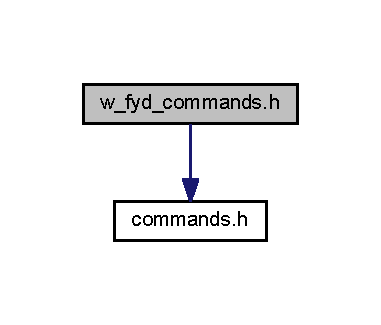
\includegraphics[width=183pt]{w__fyd__commands_8h__incl}
\end{center}
\end{figure}
This graph shows which files directly or indirectly include this file\+:
\nopagebreak
\begin{figure}[H]
\begin{center}
\leavevmode
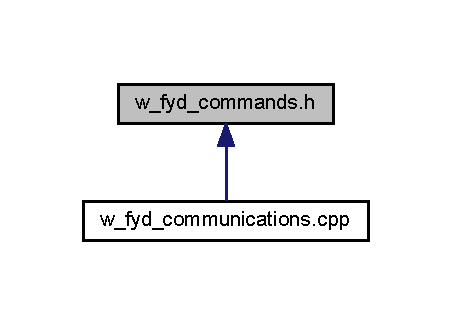
\includegraphics[width=217pt]{w__fyd__commands_8h__dep__incl}
\end{center}
\end{figure}
\subsection*{Macros}
\begin{DoxyCompactItemize}
\item 
\mbox{\label{w__fyd__commands_8h_ad97188edfdd667de971027b35330fa41}} 
\#define {\bfseries A\+P\+I\+\_\+\+V\+E\+R\+S\+I\+ON}~\char`\"{}v6.\+1.\+0 mod. W-\/F\+YD\char`\"{}
\end{DoxyCompactItemize}
\subsection*{Enumerations}
\begin{Indent}\textbf{ W-\/\+F\+YD Commands}\par
\begin{DoxyCompactItemize}
\item 
enum \textbf{ w\+\_\+fyd\+\_\+command} \{ \newline
\textbf{ C\+M\+D\+\_\+\+G\+E\+T\+\_\+\+IR} = 147, 
\textbf{ C\+M\+D\+\_\+\+S\+E\+T\+\_\+\+S\+E\+R\+VO} = 148, 
\textbf{ C\+M\+D\+\_\+\+G\+E\+T\+\_\+\+S\+E\+R\+VO} = 149, 
\textbf{ C\+M\+D\+\_\+\+G\+E\+T\+\_\+\+F\+O\+R\+CE} = 150, 
\newline
\textbf{ C\+M\+D\+\_\+\+G\+E\+T\+\_\+\+D\+U\+T\+Y\+\_\+\+C\+Y\+\_\+\+M\+AX} = 151
 \}
\end{DoxyCompactItemize}
\end{Indent}
\begin{Indent}\textbf{ W-\/\+F\+YD Parameters}\par
\begin{DoxyCompactItemize}
\item 
enum \textbf{ w\+\_\+fyd\+\_\+parameter} \{ \newline
\textbf{ P\+A\+R\+A\+M\+\_\+\+P\+O\+W\+E\+R\+\_\+\+T\+E\+N\+S\+I\+ON} = 27, 
\textbf{ P\+A\+R\+A\+M\+\_\+\+P\+U\+L\+S\+E\+\_\+\+M\+O\+D\+A\+L\+I\+TY} = 28, 
\textbf{ P\+A\+R\+A\+M\+\_\+\+S\+U\+P\+\_\+\+P\+R\+E\+S\+S\+U\+R\+E\+\_\+\+B\+O\+U\+ND} = 29, 
\textbf{ P\+A\+R\+A\+M\+\_\+\+I\+N\+F\+\_\+\+P\+R\+E\+S\+S\+U\+R\+E\+\_\+\+B\+O\+U\+ND} = 30, 
\newline
\textbf{ P\+A\+R\+A\+M\+\_\+\+P\+U\+L\+S\+E\+\_\+\+F\+R\+EQ} = 31
 \}
\end{DoxyCompactItemize}
\end{Indent}


\subsection{Detailed Description}
Definitions for W-\/\+F\+YD commands, parameters and packages. 

This file is included in the W-\/\+F\+YD firmware, in its libraries and applications. It contains all definitions that are necessary for the contruction of communication packages.

It includes definitions for all of the device commands, parameters and also the size of answer packages. 

\subsection{Enumeration Type Documentation}
\mbox{\label{w__fyd__commands_8h_ab0fb85d9785c5cc36b9017f84022c56d}} 
\index{w\+\_\+fyd\+\_\+commands.\+h@{w\+\_\+fyd\+\_\+commands.\+h}!w\+\_\+fyd\+\_\+command@{w\+\_\+fyd\+\_\+command}}
\index{w\+\_\+fyd\+\_\+command@{w\+\_\+fyd\+\_\+command}!w\+\_\+fyd\+\_\+commands.\+h@{w\+\_\+fyd\+\_\+commands.\+h}}
\subsubsection{w\+\_\+fyd\+\_\+command}
{\footnotesize\ttfamily enum \textbf{ w\+\_\+fyd\+\_\+command}}

\begin{DoxyEnumFields}{Enumerator}
\raisebox{\heightof{T}}[0pt][0pt]{\index{C\+M\+D\+\_\+\+G\+E\+T\+\_\+\+IR@{C\+M\+D\+\_\+\+G\+E\+T\+\_\+\+IR}!w\+\_\+fyd\+\_\+commands.\+h@{w\+\_\+fyd\+\_\+commands.\+h}}\index{w\+\_\+fyd\+\_\+commands.\+h@{w\+\_\+fyd\+\_\+commands.\+h}!C\+M\+D\+\_\+\+G\+E\+T\+\_\+\+IR@{C\+M\+D\+\_\+\+G\+E\+T\+\_\+\+IR}}}\mbox{\label{w__fyd__commands_8h_ab0fb85d9785c5cc36b9017f84022c56da7777ab2f7931013bfbd9b87f18c9af5a}} 
C\+M\+D\+\_\+\+G\+E\+T\+\_\+\+IR&Command for asking ir readings (W-\/\+F\+YD) \\
\hline

\raisebox{\heightof{T}}[0pt][0pt]{\index{C\+M\+D\+\_\+\+S\+E\+T\+\_\+\+S\+E\+R\+VO@{C\+M\+D\+\_\+\+S\+E\+T\+\_\+\+S\+E\+R\+VO}!w\+\_\+fyd\+\_\+commands.\+h@{w\+\_\+fyd\+\_\+commands.\+h}}\index{w\+\_\+fyd\+\_\+commands.\+h@{w\+\_\+fyd\+\_\+commands.\+h}!C\+M\+D\+\_\+\+S\+E\+T\+\_\+\+S\+E\+R\+VO@{C\+M\+D\+\_\+\+S\+E\+T\+\_\+\+S\+E\+R\+VO}}}\mbox{\label{w__fyd__commands_8h_ab0fb85d9785c5cc36b9017f84022c56da4b62947ee04d7c89f52ee16489a7d4cd}} 
C\+M\+D\+\_\+\+S\+E\+T\+\_\+\+S\+E\+R\+VO&Command for setting servo position (W-\/\+F\+YD) \\
\hline

\raisebox{\heightof{T}}[0pt][0pt]{\index{C\+M\+D\+\_\+\+G\+E\+T\+\_\+\+S\+E\+R\+VO@{C\+M\+D\+\_\+\+G\+E\+T\+\_\+\+S\+E\+R\+VO}!w\+\_\+fyd\+\_\+commands.\+h@{w\+\_\+fyd\+\_\+commands.\+h}}\index{w\+\_\+fyd\+\_\+commands.\+h@{w\+\_\+fyd\+\_\+commands.\+h}!C\+M\+D\+\_\+\+G\+E\+T\+\_\+\+S\+E\+R\+VO@{C\+M\+D\+\_\+\+G\+E\+T\+\_\+\+S\+E\+R\+VO}}}\mbox{\label{w__fyd__commands_8h_ab0fb85d9785c5cc36b9017f84022c56daf9d2d1ec0c2a99ca63697b3f4479ad54}} 
C\+M\+D\+\_\+\+G\+E\+T\+\_\+\+S\+E\+R\+VO&Command for asking servo position (W-\/\+F\+YD) \\
\hline

\raisebox{\heightof{T}}[0pt][0pt]{\index{C\+M\+D\+\_\+\+G\+E\+T\+\_\+\+F\+O\+R\+CE@{C\+M\+D\+\_\+\+G\+E\+T\+\_\+\+F\+O\+R\+CE}!w\+\_\+fyd\+\_\+commands.\+h@{w\+\_\+fyd\+\_\+commands.\+h}}\index{w\+\_\+fyd\+\_\+commands.\+h@{w\+\_\+fyd\+\_\+commands.\+h}!C\+M\+D\+\_\+\+G\+E\+T\+\_\+\+F\+O\+R\+CE@{C\+M\+D\+\_\+\+G\+E\+T\+\_\+\+F\+O\+R\+CE}}}\mbox{\label{w__fyd__commands_8h_ab0fb85d9785c5cc36b9017f84022c56dae8ddd17d302bddd6e6e2a6e186d08aba}} 
C\+M\+D\+\_\+\+G\+E\+T\+\_\+\+F\+O\+R\+CE&Command for asking force measures (W-\/\+F\+YD) \\
\hline

\raisebox{\heightof{T}}[0pt][0pt]{\index{C\+M\+D\+\_\+\+G\+E\+T\+\_\+\+D\+U\+T\+Y\+\_\+\+C\+Y\+\_\+\+M\+AX@{C\+M\+D\+\_\+\+G\+E\+T\+\_\+\+D\+U\+T\+Y\+\_\+\+C\+Y\+\_\+\+M\+AX}!w\+\_\+fyd\+\_\+commands.\+h@{w\+\_\+fyd\+\_\+commands.\+h}}\index{w\+\_\+fyd\+\_\+commands.\+h@{w\+\_\+fyd\+\_\+commands.\+h}!C\+M\+D\+\_\+\+G\+E\+T\+\_\+\+D\+U\+T\+Y\+\_\+\+C\+Y\+\_\+\+M\+AX@{C\+M\+D\+\_\+\+G\+E\+T\+\_\+\+D\+U\+T\+Y\+\_\+\+C\+Y\+\_\+\+M\+AX}}}\mbox{\label{w__fyd__commands_8h_ab0fb85d9785c5cc36b9017f84022c56da4609a5e28e724d6141584fd49b73d8a3}} 
C\+M\+D\+\_\+\+G\+E\+T\+\_\+\+D\+U\+T\+Y\+\_\+\+C\+Y\+\_\+\+M\+AX&Command for setting the max dc (W-\/\+F\+YD) \\
\hline

\end{DoxyEnumFields}
\mbox{\label{w__fyd__commands_8h_ac7c41bc61aa20dd31eb5df46bb9a1674}} 
\index{w\+\_\+fyd\+\_\+commands.\+h@{w\+\_\+fyd\+\_\+commands.\+h}!w\+\_\+fyd\+\_\+parameter@{w\+\_\+fyd\+\_\+parameter}}
\index{w\+\_\+fyd\+\_\+parameter@{w\+\_\+fyd\+\_\+parameter}!w\+\_\+fyd\+\_\+commands.\+h@{w\+\_\+fyd\+\_\+commands.\+h}}
\subsubsection{w\+\_\+fyd\+\_\+parameter}
{\footnotesize\ttfamily enum \textbf{ w\+\_\+fyd\+\_\+parameter}}

\begin{DoxyEnumFields}{Enumerator}
\raisebox{\heightof{T}}[0pt][0pt]{\index{P\+A\+R\+A\+M\+\_\+\+P\+O\+W\+E\+R\+\_\+\+T\+E\+N\+S\+I\+ON@{P\+A\+R\+A\+M\+\_\+\+P\+O\+W\+E\+R\+\_\+\+T\+E\+N\+S\+I\+ON}!w\+\_\+fyd\+\_\+commands.\+h@{w\+\_\+fyd\+\_\+commands.\+h}}\index{w\+\_\+fyd\+\_\+commands.\+h@{w\+\_\+fyd\+\_\+commands.\+h}!P\+A\+R\+A\+M\+\_\+\+P\+O\+W\+E\+R\+\_\+\+T\+E\+N\+S\+I\+ON@{P\+A\+R\+A\+M\+\_\+\+P\+O\+W\+E\+R\+\_\+\+T\+E\+N\+S\+I\+ON}}}\mbox{\label{w__fyd__commands_8h_ac7c41bc61aa20dd31eb5df46bb9a1674aa19ed4f1cc75109644c9fd0da7dda0fd}} 
P\+A\+R\+A\+M\+\_\+\+P\+O\+W\+E\+R\+\_\+\+T\+E\+N\+S\+I\+ON&Device power tension. \\
\hline

\raisebox{\heightof{T}}[0pt][0pt]{\index{P\+A\+R\+A\+M\+\_\+\+P\+U\+L\+S\+E\+\_\+\+M\+O\+D\+A\+L\+I\+TY@{P\+A\+R\+A\+M\+\_\+\+P\+U\+L\+S\+E\+\_\+\+M\+O\+D\+A\+L\+I\+TY}!w\+\_\+fyd\+\_\+commands.\+h@{w\+\_\+fyd\+\_\+commands.\+h}}\index{w\+\_\+fyd\+\_\+commands.\+h@{w\+\_\+fyd\+\_\+commands.\+h}!P\+A\+R\+A\+M\+\_\+\+P\+U\+L\+S\+E\+\_\+\+M\+O\+D\+A\+L\+I\+TY@{P\+A\+R\+A\+M\+\_\+\+P\+U\+L\+S\+E\+\_\+\+M\+O\+D\+A\+L\+I\+TY}}}\mbox{\label{w__fyd__commands_8h_ac7c41bc61aa20dd31eb5df46bb9a1674a2d48d5979e11d11d2b811295d54fbd4b}} 
P\+A\+R\+A\+M\+\_\+\+P\+U\+L\+S\+E\+\_\+\+M\+O\+D\+A\+L\+I\+TY&Pulse modality byte (W-\/\+F\+YD) \\
\hline

\raisebox{\heightof{T}}[0pt][0pt]{\index{P\+A\+R\+A\+M\+\_\+\+S\+U\+P\+\_\+\+P\+R\+E\+S\+S\+U\+R\+E\+\_\+\+B\+O\+U\+ND@{P\+A\+R\+A\+M\+\_\+\+S\+U\+P\+\_\+\+P\+R\+E\+S\+S\+U\+R\+E\+\_\+\+B\+O\+U\+ND}!w\+\_\+fyd\+\_\+commands.\+h@{w\+\_\+fyd\+\_\+commands.\+h}}\index{w\+\_\+fyd\+\_\+commands.\+h@{w\+\_\+fyd\+\_\+commands.\+h}!P\+A\+R\+A\+M\+\_\+\+S\+U\+P\+\_\+\+P\+R\+E\+S\+S\+U\+R\+E\+\_\+\+B\+O\+U\+ND@{P\+A\+R\+A\+M\+\_\+\+S\+U\+P\+\_\+\+P\+R\+E\+S\+S\+U\+R\+E\+\_\+\+B\+O\+U\+ND}}}\mbox{\label{w__fyd__commands_8h_ac7c41bc61aa20dd31eb5df46bb9a1674a446157551f6f4a7f7d7e08cabf64e1a7}} 
P\+A\+R\+A\+M\+\_\+\+S\+U\+P\+\_\+\+P\+R\+E\+S\+S\+U\+R\+E\+\_\+\+B\+O\+U\+ND&Systolic pressure value setting (W-\/\+F\+YD) \\
\hline

\raisebox{\heightof{T}}[0pt][0pt]{\index{P\+A\+R\+A\+M\+\_\+\+I\+N\+F\+\_\+\+P\+R\+E\+S\+S\+U\+R\+E\+\_\+\+B\+O\+U\+ND@{P\+A\+R\+A\+M\+\_\+\+I\+N\+F\+\_\+\+P\+R\+E\+S\+S\+U\+R\+E\+\_\+\+B\+O\+U\+ND}!w\+\_\+fyd\+\_\+commands.\+h@{w\+\_\+fyd\+\_\+commands.\+h}}\index{w\+\_\+fyd\+\_\+commands.\+h@{w\+\_\+fyd\+\_\+commands.\+h}!P\+A\+R\+A\+M\+\_\+\+I\+N\+F\+\_\+\+P\+R\+E\+S\+S\+U\+R\+E\+\_\+\+B\+O\+U\+ND@{P\+A\+R\+A\+M\+\_\+\+I\+N\+F\+\_\+\+P\+R\+E\+S\+S\+U\+R\+E\+\_\+\+B\+O\+U\+ND}}}\mbox{\label{w__fyd__commands_8h_ac7c41bc61aa20dd31eb5df46bb9a1674a6c55daf142df5d22c5c9c8cb38546a18}} 
P\+A\+R\+A\+M\+\_\+\+I\+N\+F\+\_\+\+P\+R\+E\+S\+S\+U\+R\+E\+\_\+\+B\+O\+U\+ND&Diastolic pressure value setting (W-\/\+F\+YD) \\
\hline

\raisebox{\heightof{T}}[0pt][0pt]{\index{P\+A\+R\+A\+M\+\_\+\+P\+U\+L\+S\+E\+\_\+\+F\+R\+EQ@{P\+A\+R\+A\+M\+\_\+\+P\+U\+L\+S\+E\+\_\+\+F\+R\+EQ}!w\+\_\+fyd\+\_\+commands.\+h@{w\+\_\+fyd\+\_\+commands.\+h}}\index{w\+\_\+fyd\+\_\+commands.\+h@{w\+\_\+fyd\+\_\+commands.\+h}!P\+A\+R\+A\+M\+\_\+\+P\+U\+L\+S\+E\+\_\+\+F\+R\+EQ@{P\+A\+R\+A\+M\+\_\+\+P\+U\+L\+S\+E\+\_\+\+F\+R\+EQ}}}\mbox{\label{w__fyd__commands_8h_ac7c41bc61aa20dd31eb5df46bb9a1674ae28e21f14522ad1852ebe8324c2290a3}} 
P\+A\+R\+A\+M\+\_\+\+P\+U\+L\+S\+E\+\_\+\+F\+R\+EQ&Pulse frequency setting (W-\/\+F\+YD) \\
\hline

\end{DoxyEnumFields}

\section{w\+\_\+fyd\+\_\+communications.\+cpp File Reference}
\label{w__fyd__communications_8cpp}\index{w\+\_\+fyd\+\_\+communications.\+cpp@{w\+\_\+fyd\+\_\+communications.\+cpp}}


Library of functions for serial port communication with W-\/\+F\+YD.  


{\ttfamily \#include $<$stdio.\+h$>$}\newline
{\ttfamily \#include $<$string.\+h$>$}\newline
{\ttfamily \#include $<$stdint.\+h$>$}\newline
{\ttfamily \#include $<$ctype.\+h$>$}\newline
{\ttfamily \#include $<$time.\+h$>$}\newline
{\ttfamily \#include $<$unistd.\+h$>$}\newline
{\ttfamily \#include $<$fcntl.\+h$>$}\newline
{\ttfamily \#include $<$errno.\+h$>$}\newline
{\ttfamily \#include $<$termios.\+h$>$}\newline
{\ttfamily \#include $<$sys/ioctl.\+h$>$}\newline
{\ttfamily \#include $<$dirent.\+h$>$}\newline
{\ttfamily \#include $<$sys/time.\+h$>$}\newline
{\ttfamily \#include $<$stdlib.\+h$>$}\newline
{\ttfamily \#include $<$linux/serial.\+h$>$}\newline
{\ttfamily \#include \char`\"{}w\+\_\+fyd\+\_\+communications.\+h\char`\"{}}\newline
{\ttfamily \#include \char`\"{}w\+\_\+fyd\+\_\+commands.\+h\char`\"{}}\newline
Include dependency graph for w\+\_\+fyd\+\_\+communications.\+cpp\+:
\nopagebreak
\begin{figure}[H]
\begin{center}
\leavevmode
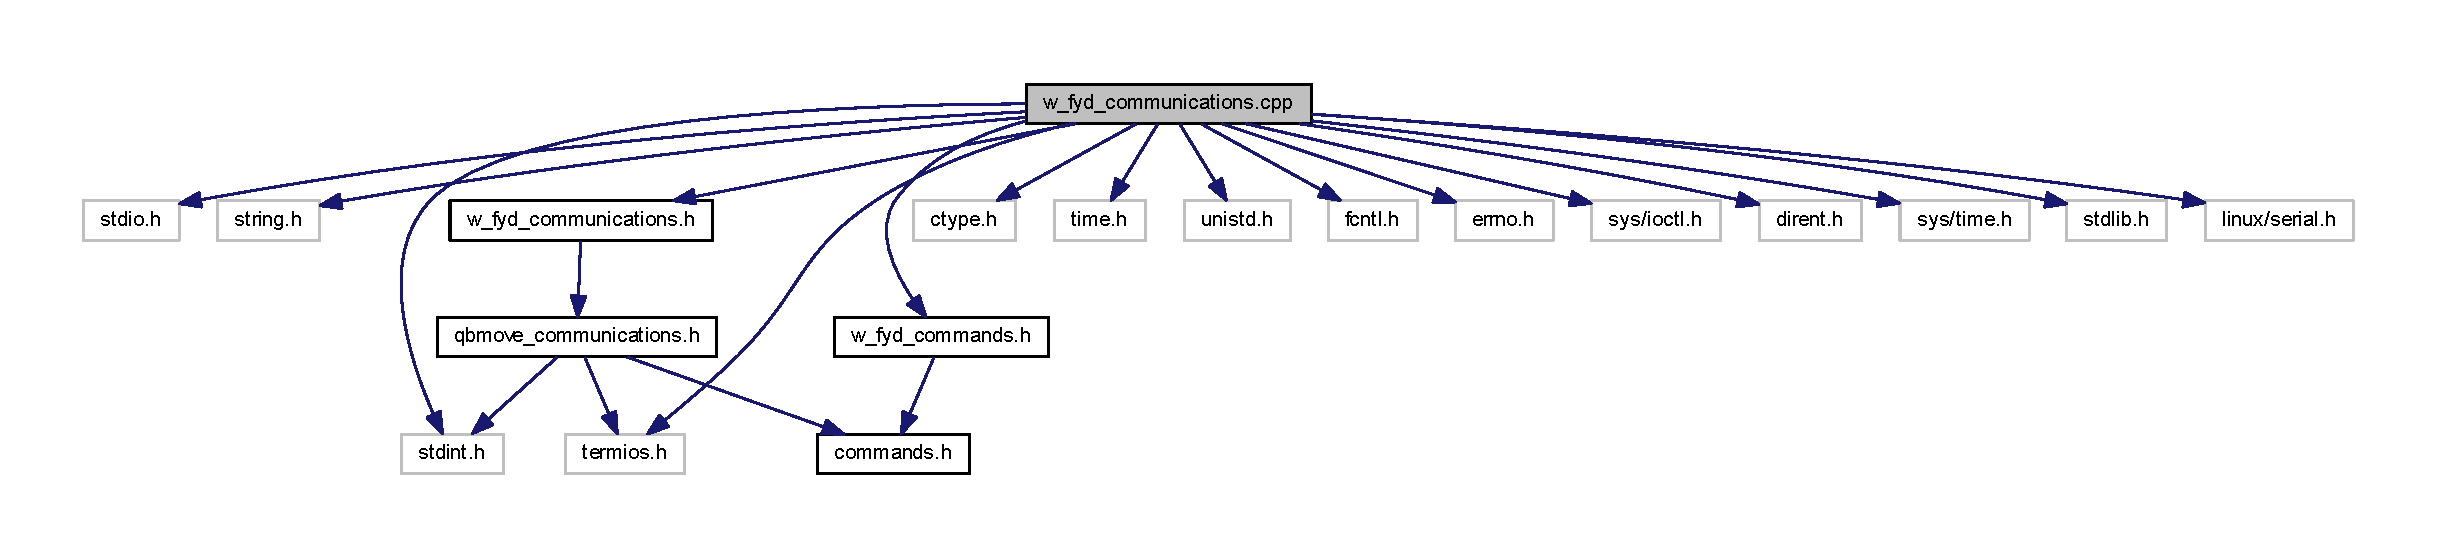
\includegraphics[width=350pt]{w__fyd__communications_8cpp__incl}
\end{center}
\end{figure}
\subsection*{Macros}
\begin{DoxyCompactItemize}
\item 
\mbox{\label{w__fyd__communications_8cpp_a6b20d41d6252e9871430c242cb1a56e7}} 
\#define \textbf{ B\+U\+F\+F\+E\+R\+\_\+\+S\+I\+ZE}~500
\begin{DoxyCompactList}\small\item\em Size of buffers that store communication packets. \end{DoxyCompactList}\end{DoxyCompactItemize}


\subsection{Detailed Description}
Library of functions for serial port communication with W-\/\+F\+YD. 

\begin{DoxyDate}{Date}
October 01, 2017 
\end{DoxyDate}
\begin{DoxyAuthor}{Author}
{\itshape Centro \char`\"{}\+E.\+Piaggio\char`\"{}} 
\end{DoxyAuthor}
\begin{DoxyCopyright}{Copyright}
(C) 2012-\/2016 qbrobotics. All rights reserved. 

(C) 2017 Centro \char`\"{}\+E.\+Piaggio\char`\"{}. All rights reserved.
\end{DoxyCopyright}
Check the \doxyref{w\+\_\+fyd\+\_\+communications.h}{p.}{w__fyd__communications_8h} file for a complete description of the public functions implemented in \doxyref{w\+\_\+fyd\+\_\+communications.\+cpp}{p.}{w__fyd__communications_8cpp}. 
\section{w\+\_\+fyd\+\_\+communications.\+h File Reference}
\label{w__fyd__communications_8h}\index{w\+\_\+fyd\+\_\+communications.\+h@{w\+\_\+fyd\+\_\+communications.\+h}}


Library of functions for S\+E\+R\+I\+AL P\+O\+RT communication with W\+F\+YD. Function Prototypes.  


{\ttfamily \#include \char`\"{}qbmove\+\_\+communications.\+h\char`\"{}}\newline
Include dependency graph for w\+\_\+fyd\+\_\+communications.\+h\+:
\nopagebreak
\begin{figure}[H]
\begin{center}
\leavevmode
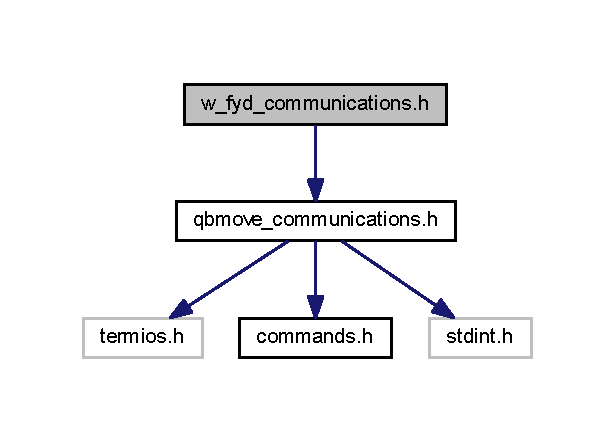
\includegraphics[width=295pt]{w__fyd__communications_8h__incl}
\end{center}
\end{figure}
This graph shows which files directly or indirectly include this file\+:
\nopagebreak
\begin{figure}[H]
\begin{center}
\leavevmode
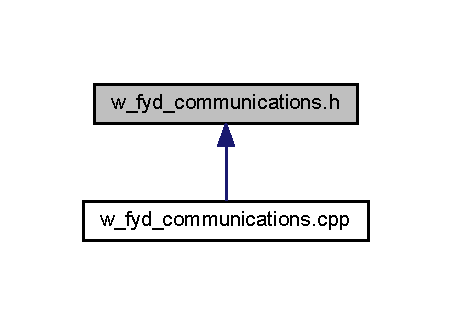
\includegraphics[width=217pt]{w__fyd__communications_8h__dep__incl}
\end{center}
\end{figure}
\subsection*{Functions}
\begin{DoxyCompactItemize}
\item 
\mbox{\label{w__fyd__communications_8h_a9e9e8a0bb8644a0de99085f33faa1ac9}} 
int {\bfseries comm\+Get\+IR} (\textbf{ comm\+\_\+settings} $\ast$comm\+\_\+settings\+\_\+t, int id, short int measurements[1])
\item 
\mbox{\label{w__fyd__communications_8h_a10d1a5e2641255a2bcf56d5fb60bdfda}} 
void {\bfseries comm\+Set\+Servo} (\textbf{ comm\+\_\+settings} $\ast$comm\+\_\+settings\+\_\+t, int id, short int inputs[1])
\item 
\mbox{\label{w__fyd__communications_8h_ac07d3498ca20b672831a597a0ac63369}} 
int {\bfseries comm\+Get\+Servo} (\textbf{ comm\+\_\+settings} $\ast$comm\+\_\+settings\+\_\+t, int id, short int measurements[1])
\item 
\mbox{\label{w__fyd__communications_8h_a02a9df4bac7885c5f10c70617df705a8}} 
int {\bfseries comm\+Get\+Force} (\textbf{ comm\+\_\+settings} $\ast$comm\+\_\+settings\+\_\+t, int id, short int measurements[1])
\item 
\mbox{\label{w__fyd__communications_8h_a3fc8bc2506b1e918938d08c3539813d1}} 
int {\bfseries comm\+Get\+D\+CyM} (\textbf{ comm\+\_\+settings} $\ast$comm\+\_\+settings\+\_\+t, int id, short int measurements[1])
\end{DoxyCompactItemize}


\subsection{Detailed Description}
Library of functions for S\+E\+R\+I\+AL P\+O\+RT communication with W\+F\+YD. Function Prototypes. 

\begin{DoxyDate}{Date}
October 01, 2017 
\end{DoxyDate}
\begin{DoxyAuthor}{Author}
{\itshape Centro \char`\"{}\+E.\+Piaggio\char`\"{}} 
\end{DoxyAuthor}
\begin{DoxyCopyright}{Copyright}
(C) 2012-\/2016 qbrobotics. All rights reserved. 

(C) 2017 Centro \char`\"{}\+E.\+Piaggio\char`\"{}. All rights reserved.
\end{DoxyCopyright}
This library contains all necessary functions for communicating with W\+F\+YD when using a U\+SB to R\+S485 connector that provides a Virtual C\+OM interface. 
%--- End generated contents ---

% Index
\backmatter
\newpage
\phantomsection
\clearemptydoublepage
\addcontentsline{toc}{chapter}{Index}
\printindex

\end{document}
